\documentclass[11pt,a4paper]{article}
\usepackage[margin=2.3cm]{geometry}
\usepackage{lmodern}        % classic Computer Modern look, vectorized (T1)
\usepackage[T1]{fontenc}
\usepackage{amsmath,amssymb}
\usepackage{graphicx}
\graphicspath{{figures/}}
\usepackage{xcolor}
\usepackage{booktabs}
\usepackage{longtable}
\usepackage{fancyhdr}
\setlength{\headheight}{14pt}   % silence fancyhdr's headheight warning
\usepackage{titlesec}
% Cross-document references for the split JNE build: the article cites
% supplementary figures and the supplement cites main-text sections and
% equations. xr-hyper (not xr) is the hyperref-compatible version and must be
% loaded BEFORE hyperref. `./build.sh all` is run twice so the numbers settle.
\usepackage{xr-hyper}
\usepackage[hidelinks]{hyperref}
\usepackage{caption}
\usepackage{enumitem}
\captionsetup{font=small,labelfont=bf}
\usepackage{parskip}

% ---------------------------------------------------------------------------
% Build switch. \jnefalse -> Neuroelectrics/BCOM Technical Note (TN0484/WP0185).
%                \jnetrue  -> Journal of Neural Engineering manuscript.
% One source, two outputs: the TN keeps its branding and the full appendices;
% the JNE build strips the house furniture and uses the structured abstract.
% Never fork this file -- switch the flag.
%
% Default is the TN. Select the JNE build from the command line, without
% editing this file, via ./build.sh jne  (which invokes pdflatex as
%   pdflatex -jobname=TN0484_jne "\def\jnebuild{}\input{<this file>}" ).
% ---------------------------------------------------------------------------
\newif\ifjne
\jnefalse
\ifdefined\jnebuild\jnetrue\fi

% ---------------------------------------------------------------------------
% Supplement switch. \supptrue -> build ONLY the appendices and supplementary
% figures, as a standalone companion file. Selected from the command line via
%   ./build.sh supp
% JNE counts the main article against a ~12,000-word guideline; splitting the
% back matter into a separate file brings the article itself under it without
% removing any content. The TN build (neither flag) keeps everything in one PDF.
% ---------------------------------------------------------------------------
\newif\ifsupp
\suppfalse
\ifdefined\suppbuild\supptrue\jnetrue\fi

% appendices travel with the TN build and with the supplement, but not with the
% standalone JNE article
\newif\ifappendices
\ifsupp\appendicestrue\else\ifjne\appendicesfalse\else\appendicestrue\fi\fi

\ifjne
  \ifsupp
    \IfFileExists{TN0484_jne.aux}{\externaldocument{TN0484_jne}}{}
  \else
    \IfFileExists{TN0484_jne_supplement.aux}{\externaldocument{TN0484_jne_supplement}}{}
  \fi
\fi

\definecolor{neblue}{RGB}{10,79,140}
\definecolor{negray}{RGB}{85,85,85}
\definecolor{nered}{RGB}{179,54,31}

\ifjne
  % Plain black headings; IOP typesets its own styling at production.
  \titleformat{\section}{\large\bfseries}{\thesection}{0.6em}{}
  \titleformat{\subsection}{\normalsize\bfseries}{\thesubsection}{0.6em}{}
  \pagestyle{plain}
\else
  \titleformat{\section}{\large\bfseries\color{neblue}}{\thesection}{0.6em}{}
  \titleformat{\subsection}{\normalsize\bfseries\color{negray}}{\thesubsection}{0.6em}{}
  \pagestyle{fancy}\fancyhf{}
  \lhead{\textcolor{neblue}{\textbf{NEUROELECTRICS/BCOM}}\ \textcolor{negray}{\small Technical Note}}
  \rhead{\textcolor{negray}{\small TN0484\,/\,WP0185}}
  \lfoot{\textcolor{negray}{\scriptsize Neuroelectrics / BCOM --- Preprint}}
  \rfoot{\textcolor{negray}{\scriptsize \thepage}}
  \renewcommand{\headrulewidth}{0.8pt}
  \renewcommand{\footrulewidth}{0.4pt}
\fi

\newcommand{\Sig}{\sigma}
\newcommand{\half}{\tfrac{1}{2}}

\begin{document}

\ifjne
% ---------------------------------------------------------------------------
% TODO before submission: confirm affiliations 3 and 4 with Canals and Mirasso
% (reconstructed from the Overleaf edit plus the Zenodo deposit, not yet checked
% by them); confirm corresponding-author email. ORCIDs below verified against
% the ORCID registry (2026-07-21).
% ---------------------------------------------------------------------------
\begin{center}
{\LARGE\bfseries The cortical column as a tuned receiver:\\[4pt]
a network mechanism for temporal-interference stimulation}\\[16pt]
{\large Giulio Ruffini$^{1,2}$, Borja Mercadal$^{1}$, Alex Just$^{1}$,
Raul de Palma Aristides$^{2}$,\\[2pt]
Francesca Castaldo$^{1,2}$, Santiago Canals$^{2,4}$, and Claudio Mirasso$^{2,3}$}\\[12pt]
\begin{minipage}{0.86\textwidth}\centering\small
$^{1}$Neuroelectrics, Barcelona, Spain\\
$^{2}$BCOM, Barcelona, Spain\\
$^{3}$IFISC (UIB-CSIC), Palma de Mallorca, Spain\\
$^{4}$Instituto de Neurociencias (UMH-CSIC), Sant Joan d'Alacant, Spain\\[6pt]
E-mail: \texttt{giulio.ruffini@neuroelectrics.com}
\end{minipage}\\[8pt]
\begin{minipage}{0.86\textwidth}\centering\footnotesize\color{negray}
\textbf{ORCID iDs:}\ %
G.~Ruffini \href{https://orcid.org/0000-0003-3084-0177}{0000-0003-3084-0177};\ %
B.~Mercadal \href{https://orcid.org/0000-0002-0941-6796}{0000-0002-0941-6796};\ %
A.~Just \href{https://orcid.org/0009-0006-8794-7425}{0009-0006-8794-7425};\ %
R.~de Palma Aristides \href{https://orcid.org/0000-0002-0255-2293}{0000-0002-0255-2293};\ %
F.~Castaldo \href{https://orcid.org/0000-0002-4947-4552}{0000-0002-4947-4552};\ %
S.~Canals \href{https://orcid.org/0000-0003-2175-8139}{0000-0003-2175-8139};\ %
C.~Mirasso \href{https://orcid.org/0000-0003-2980-7038}{0000-0003-2980-7038}.
\end{minipage}
\end{center}
\vspace{6pt}
\else
\begin{flushleft}
{\color{neblue}\rule{\textwidth}{2pt}}\\[4pt]
{\LARGE\bfseries The cortical column as a tuned receiver:\\[2pt]
a network mechanism for temporal-interference stimulation}\\[10pt]
\begin{tabular}{@{}ll@{}}
\textbf{Document:} & TN0484 (Neuroelectrics TN)\,/\,WP0185 (BCOM WP) \\
\textbf{Author:} & Giulio Ruffini, Borja Mercadal, Alex Just, Raul de Palma Aristides,\\
& Francesca Castaldo, Santiago Canals, and Claudio Mirasso \\
\textbf{Affiliation:} & Neuroelectrics\,/\,BCOM\,/\,IFISC (UIB-CSIC)\,/\,IN (UMH-CSIC) \\
\textbf{Date:} & 2026-07-21 \qquad \textbf{Version:} 0.12.0 \\
\textbf{DOI:} & \href{https://doi.org/10.5281/zenodo.21009618}{10.5281/zenodo.21009618} \\
\end{tabular}\\[4pt]
{\color{neblue}\rule{\textwidth}{1pt}}
\end{flushleft}
\fi

\ifsupp
\begin{center}
{\large\bfseries Supplementary Material}\\[4pt]
\begin{minipage}{0.86\textwidth}\centering\small
Appendices and supplementary figures accompanying the article. Section, equation and
figure numbers referenced here follow the main text; supplementary figures are numbered
S1, S2, \dots
\end{minipage}
\end{center}
\vspace{8pt}
\fi

\ifsupp\else
\section*{Abstract}
\ifjne
% JNE structured abstract: Objective / Approach / Main results / Significance,
% bold run-in headings, 300-word cap. Currently 292 -- any addition needs a cut.
\noindent
\textbf{Objective.} Temporal-interference (TI) stimulation applies two high-frequency
currents whose amplitudes beat at a low difference frequency, offering focal, steerable
stimulation deep in the brain. Yet an amplitude-modulated field carries no spectral power
at the beat frequency, so no passive, linear element of a neuron can follow it. Recovering the beat requires a nonlinearity, which has generally been sought
in single-cell ion channels. We ask whether demodulation and its frequency tuning are
instead properties of the neural population.
\textbf{Approach.} We treat the firing-rate nonlinearity of a neural mass, the
$\sim$$10^4$-neuron unit that generates the EEG, as an amplitude detector, and its recurrent
synaptic network poised near a Hopf bifurcation as a resonant amplifier. The account is
tested across a modeling ladder: a heuristic Jansen--Rit column (JR), a laminar model (LaNMM), an
exact next-generation mean field (NMM2), and the quadratic integrate-and-fire spiking
network underlying it.
\textbf{Main results.} Population transfer function (sigmoid in JR) curvature acts as a square-law detector that recovers the
beat, and the network amplifies it resonantly at its own natural frequency. Detection is
inherited from the single neuron; the sharp frequency selectivity is emergent, set by
proximity to criticality and tunable by connectivity. The mechanism reproduces TI's known
behavior: independence of the carrier once membrane polarization is matched, largest
response when the beat matches a region's intrinsic rhythm, and, because the resonance
amplifies oscillatory timing far more than mean rate, realignment of spike timing with only
a small change in firing rate, as observed in vivo.
\textbf{Significance.} TI efficacy should be as much a property of the brain as of the
device, depending on brain state and regional connectivity. The cortical column behaves as a
tuned AM radio receiver, which reframes dose optimization around the target's dynamics and
yields falsifiable predictions listed in the paper.
\else
\noindent
Temporal-interference (TI) stimulation promises what other non-invasive methods
cannot: focal, steerable stimulation deep in the brain, produced where two
high-frequency currents overlap and their amplitudes beat at a low difference
frequency. Yet an amplitude-modulated field carries no
power at that beat frequency, so no passive, linear part of a neuron can follow it;
recovering the beat requires a nonlinearity, usually sought in single-cell ion
channels. Here we show that the recovery, and its tuning, are properties of the neural
\emph{population} rather than the single cell. In a neural mass, the
$\sim$$10^4$-neuron unit that generates the EEG, the firing-rate nonlinearity acts as
a square-law detector that demodulates the beat, while the recurrent synaptic network,
poised near a Hopf bifurcation, resonantly amplifies the recovered rhythm at its own
natural frequency. Detection is inherited from the single neuron; the sharp,
frequency-selective amplification is emergent, set by how near the network sits to
criticality and tunable by its own connectivity. Demonstrated in a heuristic cortical
column and in an exact next-generation mean field, the mechanism reproduces TI's known
behavior: it is independent of the carrier once the membrane polarization is matched,
largest when the beat matches a region's intrinsic rhythm, and, because the resonance
amplifies oscillatory timing far more than mean rate, it locks spike timing with only a
small change in firing rate, as observed in vivo. Because the gain depends on brain state, TI
efficacy should be as much a property of the brain as of the device: the cortical
column behaves as a tuned AM radio receiver.
\fi

\smallskip
\noindent\textbf{Keywords:} temporal interference; non-invasive neuromodulation;
transcranial stimulation; neural mass model; amplitude demodulation; Hopf bifurcation;
cross-frequency coupling; criticality.

% Kept in both builds: reviewers use the contents list to navigate.
\clearpage
\tableofcontents
\clearpage

\section{Introduction}
Reaching a deep brain target without stimulating the tissue above it is a long-standing
goal of non-invasive neuromodulation, and temporal-interference (TI) stimulation
\cite{grossman2017} is its most prominent recent proposal. TI applies two sinusoids at
$f_1$ and $f_2=f_1+\Delta f$ through separate electrode pairs (typically
$f_1\!\sim\!1$--$2$~kHz, $\Delta f\!\sim\!1$--$100$~Hz). Where the two fields
overlap, their superposition is an AM signal whose carrier is near $f_1$ and
whose envelope beats at the difference frequency $\Delta f$. The appeal is
spatial: the envelope amplitude peaks in a focal, steerable region at depth,
while superficial tissue sees only the (putatively inert) kHz carrier---a promise
of non-invasive, focal, deep stimulation that explains the intense interest.

The difficulty is conceptual rather than technological. Write the field as
\begin{equation}
s(t)=\varepsilon\,[\,1+m\cos(\Omega t)\,]\cos(\omega_c t),\qquad
\omega_c=2\pi f_c,\quad \Omega=2\pi\,\Delta f ,
\label{eq:am}
\end{equation}
where $m$ is the modulation depth, $\Delta f$ the envelope (beat) frequency, $f_c$
the carrier frequency (the mean $(f_1+f_2)/2$ of the two applied tones, the envelope
beating at their difference $\Delta f=f_2-f_1$), and $\varepsilon$ the field amplitude
(refined to the post-coupling polarization in \S\ref{sec:coupling}); its spectrum has support
\emph{only} at $\omega_c$ and $\omega_c\pm\Omega$
(Fig.~\ref{fig:demod}): there is no energy at the envelope frequency $\Omega$. A
linear, time-invariant (LTI) system maps a sinusoid to a sinusoid of the same
frequency; it can attenuate or phase-shift the three carrier lines but can
\emph{never} synthesize a new line at $\Omega$. The membrane's passive RC
low-pass---often invoked as ``the neuron follows the slow envelope''---therefore
cannot by itself demodulate TI. Demodulation requires a nonlinearity. This is
the founding lesson of AM radio \cite{nahin2001}: a receiver cannot
recover the message with linear components alone; it needs a nonlinear element (a
square-law device or a diode) to shift spectral energy down to \emph{baseband}---the
low-frequency band near $0$~Hz where the message lives---followed by a tuned filter to
select the station and a low-pass to read the envelope.

Where, then, is the nonlinearity in the brain? The original passive-filtering
intuition is now widely regarded as insufficient, since a linear filter cannot
create the envelope line \cite{mirzakhalili2020}. The leading biophysical account
places the nonlinearity in single-neuron ion channels: Mirzakhalili et al.\
\cite{mirzakhalili2020} show in Hodgkin--Huxley/Frankenhaeuser--Huxley axon models
that TI works through nonlinear, ion-channel-mediated rectification, in which
asymmetric voltage-gated conductances rectify the carrier and, after membrane
low-pass, follow the envelope---the textbook rectify-then-filter detector. Other
studies report that TI thresholds inherit the carrier's frequency dependence,
suggesting a mechanism shared with direct kHz stimulation (conduction block,
onset response) rather than a dedicated envelope channel
\cite{opancar2025,peripheral2023}, and in some peripheral preparations the
response is not driven by envelope extraction at all \cite{peripheral2023}. In
vivo, TI reliably alters spike \emph{timing} but not firing rate in the primate
brain, and is much weaker than conventional low-frequency stimulation under
human-relevant conditions \cite{vieira2024}. Most tellingly, recent slice work
finds that pyramidal and parvalbumin (PV) interneurons respond differently and
that most pyramidal TI responses disappear when synaptic transmission is blocked,
leading Caldas-Martinez et al.\ to conclude that TI is ``largely a network
phenomenon'' \cite{caldas2024}; computational network models point the same way
\cite{soroushi2025}.

Here we show that a population-scale mechanism, built from two ingredients already in
standard cortical models, suffices: a static firing-rate \emph{sigmoid}, whose
nonzero curvature $\Sig''$ makes it a square-law demodulator, and a
\emph{second-order-synapse network} whose synaptic kinetics filter the carrier away
while a weakly-damped \emph{stable focus} resonantly amplifies the recovered beat component at
the network's natural frequency (Fig.~\ref{fig:concept}). The amplification is a property
of the focus, not of the Hopf specifically: it sharpens as the focus nears criticality,
which the column approaches near \emph{both} the saddle-node on an invariant circle
(SNIC, a slower rhythm) and the Hopf
(alpha). Where existing accounts locate the nonlinearity in cellular excitability, ours reads
it out at the mesoscopic scale: the sigmoid is a coarse-grained summary of the
population's single-cell input--output curves, but once coarse-grained it is a
\emph{distinct mesoscopic nonlinearity} with enough curvature to detect envelopes,
whatever microscopic mechanism supplies it. This is a network-level mechanism for TI
demodulation---carrier-independent (at fixed polarization) and
frequency-selective---complementary to the disinhibitory network effect
(PV-interneuron silencing) reported by \cite{caldas2024}; both place TI's action in the
population rather than the single cell. We develop it first in a single Jansen--Rit column,
analyzable in closed form, then in the two-band laminar model (LaNMM), whose own alpha
and gamma loops bring it closer to cortex, and finally in an exact next-generation mean
field, where the demodulating nonlinearity is derived rather than assumed.

This work builds on a line of research in which neural-mass models implement
AM-radio principles \emph{internally}, for the brain's own signals. In our
cross-frequency-coupling account of predictive coding \cite{ruffini2025cfc}, the
LaNMM realizes a columnar Comparator through sigmoid-enabled signal-to-envelope
(SEC) and envelope-to-envelope (EEC) couplings, where error evaluation is literally
demodulation---the sign-reversed prediction ``un-modulates'' the carrier. The
Hierarchical Amplitude Modulation (HAM) framework \cite{ruffini2025ham} generalizes
this to nested envelopes with constant-$Q$ (log-spaced) bands, a candidate origin of
$1/f$ spectra---again through the sigmoid's quadratic cross-term. The present work
turns this machinery outward: if the cortex is an AM transceiver for its own rhythms,
it can also be an AM receiver for an external carrier.

\begin{figure}[t!]
\centering
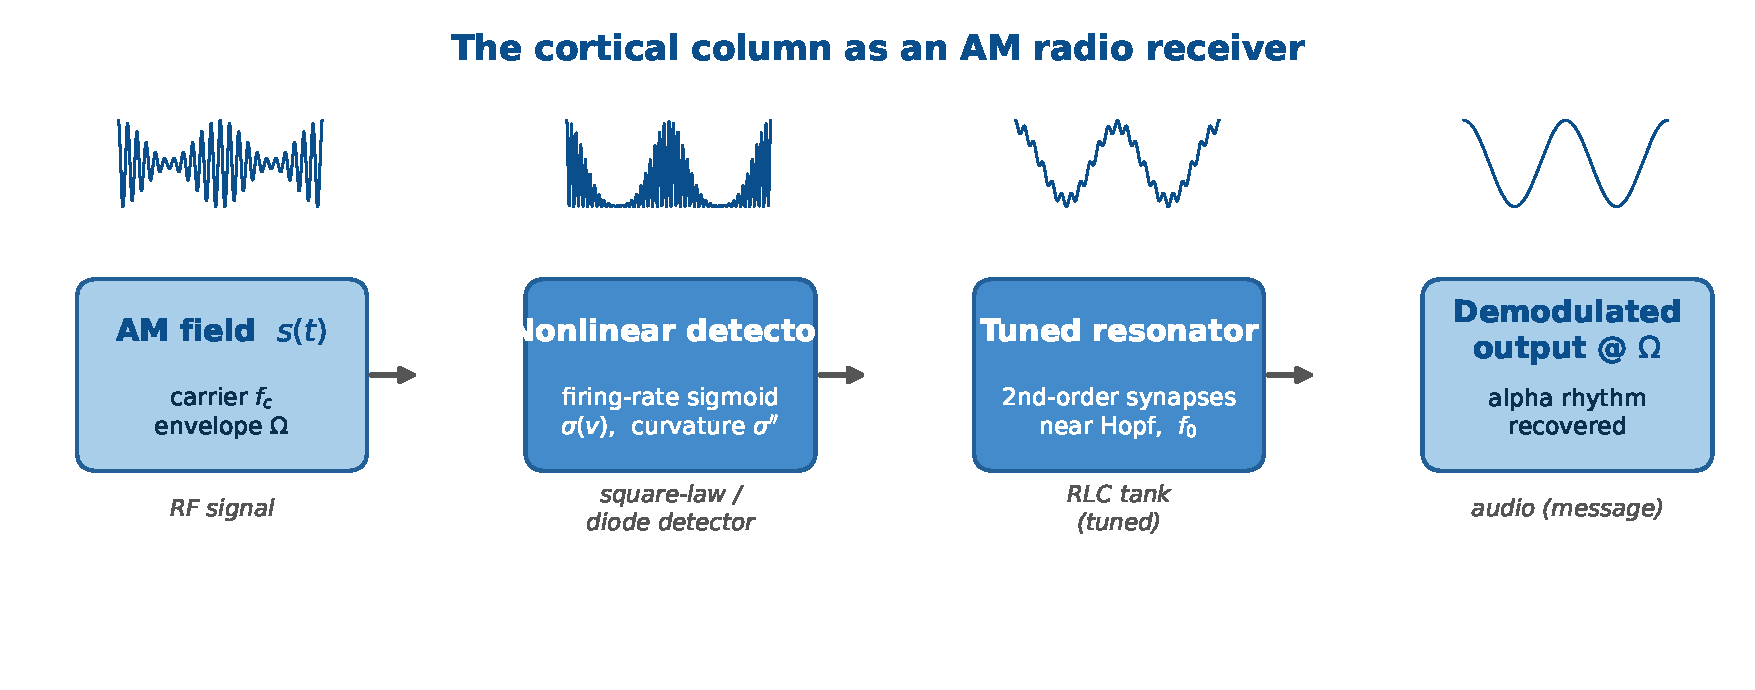
\includegraphics[width=\textwidth]{fig_concept.pdf}
%\vspace{-2cm}

\caption{\textbf{The cortical column as an AM radio receiver (schematic).} An AM field
(carrier $f_c$, envelope $\Omega$) reaches a nonlinear detector (the firing-rate
sigmoid, curvature $\Sig''$), whose output passes through a tuned resonator (the
second-order-synapse network near a Hopf, natural frequency $f_0$), recovering
a beat-frequency component as an oscillation at $\Omega$. The stages map onto the radio-frequency (RF)
front end, square-law/diode detector, resonant RLC tank (the tuned
resistor--inductor--capacitor circuit that selects one station), and audio output of a
classic AM receiver
\cite{nahin2001}. The firing-rate sigmoid plays the role of the detector; the
second-order-synapse network near a Hopf is the tuned tank that selects and
amplifies a particular envelope frequency, so TI ``broadcasts'' to whichever
columns are tuned to its beat frequency.}
\label{fig:concept}
\end{figure}

\section{Theory}

\subsection{Neural mass models and the Jansen--Rit circuit}\label{sec:nmm}
A neural mass model (NMM) collapses the activity of a large population
($\sim$$10^4$) of similar neurons into a handful of population-averaged variables
\cite{ruffini2025rosetta,jansen1995}. Two elements recur in every such model.
First, each synapse acts as a \emph{linear filter} $\hat K$ that converts an
incoming presynaptic firing rate $r(t)$ into a postsynaptic potential (PSP)
$x(t)=\hat K[r]$; equivalently $r=\hat L[x]$ with $\hat L=\hat K^{-1}$ a
differential operator whose few coefficients set the synapse's gain, decay time
and delay \cite{ruffini2025rosetta}. In the Jansen--Rit (JR) family the kernel is
the ``alpha function'' $h(t)=Aa\,t\,e^{-at}$ (excitatory; $B,b$ for the inhibitory
synapse), i.e.\ the second-order operator
$\hat L=(Aa)^{-1}(\mathrm{d}/\mathrm{d}t+a)^2$, so each PSP obeys
$\ddot x+2a\dot x+a^2x = Aa\,r(t)$. Second, the PSPs converging on a population sum
to a mean membrane potential $v=\sum_s x_s$, which a static, saturating
\emph{transfer function}---the sigmoid---turns back into a population firing rate
\cite{wilsoncowan1972},
\begin{equation}
\Sig(v)=\frac{2e_0}{1+e^{\,\rho(v_0-v)}} ,
\label{eq:sigmoid}
\end{equation}
with maximal firing rate $2e_0$, half-maximal at the inflection $v_0$, and slope set by
$\rho$; it saturates because firing rates are bounded \cite{ruffini2025rosetta}. The sigmoid is
the only nonlinearity in the model, and---as we show---it is what makes
(de)modulation possible. Its curvature, which does the demodulating, originates in
the single neuron's own input--output nonlinearity: $\Sig$ is the mean-field
(ensemble) average of single-neuron transfer curves over a heterogeneous, noisy
population, so $\Sig''$ is inherited from single cells and only reshaped---smoothed
and broadened---by the spread of states, thresholds and noise: the curvature is
cellular in origin, but its demodulation is read out at the population level by the
generic sigmoid, while the network supplies the resonant \emph{amplification} we use here
(\S\ref{sec:carrier}). Frequency-selective resonance can also be intrinsic to single cells
(e.g.\ $I_h$ and $I_M$ currents \cite{hutcheonyarom2000}); we locate it instead in the
network, where second-order synapses near criticality generate it even when the cells do
not \cite{brunelhakim1999,brunelwang2003}.

This becomes exact one rung up the modeling ladder \cite{ruffini2025rosetta}. For a
network of all-to-all coupled quadratic integrate-and-fire (QIF) neurons with
Lorentzian-distributed excitabilities, the Ott--Antonsen ansatz yields a
\emph{closed, exact} mean field for the population firing rate $r$ and mean
potential $v$---the next-generation (Montbri\'o--Paz\'o--Roxin, MPR) mass
\cite{montbrio2015}, completed with the second-order synapses of neural-mass models
in the exact ``NMM2'' theory \cite{ruffini2021nmm2,clusella2023}:
\begin{equation}
\dot r=\frac{\Delta}{\pi}+2rv,\qquad
\dot v=v^2+\bar\eta-\pi^2 r^2+I(t),
\label{eq:mpr}
\end{equation}
with the applied current $I(t)$ entering linearly, the common background excitability
$\bar\eta$ (the bifurcation parameter), and the heterogeneity half-width
$\Delta$ setting the smoothing. Here the demodulating nonlinearity is \emph{derived,
not postulated}: the quadratic $v^2$ term (with the $rv$ coupling) is an exact
square-law rectifier of the input, inherited directly from the single-neuron QIF
dynamics. The Jansen--Rit sigmoid is the heuristic (NMM1) stand-in for this
transfer---exact in the slow-synapse limit \cite{clusella2023}---so our square-law
result is a generic property of the mean field, not an artifact of expanding one
postulated curve. The same exact theory already exhibits weak-field resonance and
Arnold tongues that sharpen with self-coupling \cite{clusella2023,ruffini2021nmm2},
the near-Hopf amplification we exploit below.

\emph{What the transfer functions represent.} In every model the demodulating object is a
\emph{population} input--output map rather than a passive somatic membrane element. In JR/LaNMM it
is the sigmoid \eqref{eq:sigmoid}, the effective transfer of an excitable neuronal ensemble
(mean PSP in, population firing rate out); in NMM2 the same role is played by the exact MPR
quadratic \eqref{eq:mpr}. Its curvature is the mesoscopic trace of cellular nonlinearities
(thresholds, spike generation, refractoriness, noise, saturation), so reading the
demodulation off $\Sig''$, or off the derived $v^2$ term, is legitimate at this scale. The
membrane low-pass does not contradict this: it bears on \emph{access}, not legitimacy. The
open biophysical question is which fast compartment (axon initial segment, node, terminal,
or channel) lets a kHz carrier reach that nonlinear transfer (\S\ref{sec:khz}); once the
carrier is sampled there, the neural mass describes the population-level demodulation and
near-Hopf amplification of the recovered beat component.

The single-column JR circuit couples a pyramidal population to one excitatory and
one inhibitory interneuron population through this synapse$+$sigmoid motif. Writing
$y_0$ for the excitatory PSP driving the interneurons, $y_1$ and $y_2$ for the
excitatory and inhibitory PSPs onto the pyramidal population, and the
local-field-potential (LFP) proxy $v=y_1-y_2$, with external input $p$,
\begin{align}
\ddot y_0 &= Aa\,\Sig\!\big(y_1-y_2+s(t)\big)-2a\dot y_0-a^2 y_0, \label{eq:jr0}\\
\ddot y_1 &= Aa\,\big[\,p+C_2\,\Sig(C_1 y_0)\,\big]-2a\dot y_1-a^2 y_1,\\
\ddot y_2 &= Bb\,C_4\,\Sig(C_3 y_0)-2b\dot y_2-b^2 y_2,
\end{align}
integrated as six first-order ODEs with the parameters of Table~\ref{tab:params}
\cite{jansen1995}. The term $s(t)$ is the applied-field perturbation, introduced
next; the read-out is $v=y_1-y_2$.

\begin{table}[t!]\centering\small
\caption{Jansen--Rit parameters \cite{jansen1995}.}
\label{tab:params}
\begin{tabular}{@{}lll@{}}
\toprule
Symbol & Meaning & Value\\
\midrule
$A,\,B$ & excit./inhib.\ PSP gain & $3.25,\ 22$ mV\\
$a,\,b$ & synaptic rates & $100,\ 50$ s$^{-1}$\\
$v_0,\,e_0,\,\rho$ & sigmoid inflection, max rate$/2$, slope & $6$ mV, $2.5$ s$^{-1}$, $0.56$ mV$^{-1}$\\
$C$ & global connectivity & $135$\\
$C_1,C_2,C_3,C_4$ & couplings & $C,\,0.8C,\,0.25C,\,0.25C$\\
$p$ & external input (bifurcation knob) & $0$--$400$ Hz\\
\bottomrule
\end{tabular}
\end{table}

For the biophysical realization (\S\ref{sec:lanmm-results}) we use a second model
built from the same ingredients: the laminar neural mass model (LaNMM)
\cite{ruffini2025cfc,sanchezTodo2023}, which embeds this synapse$+$sigmoid motif in
a two-band cortical column---a deep Jansen--Rit-like subcircuit (pyramidal $P_1$
with spiny-stellate (SS) and somatostatin (SST) interneurons; intrinsic alpha,
$\sim$10~Hz) coupled to a superficial PING-like (pyramidal--interneuron network
gamma) subcircuit (pyramidal $P_2$ with PV interneurons; intrinsic gamma,
$\sim$40~Hz). The single JR column lets us isolate and analyze the
mechanism; the LaNMM then exhibits it in a column with its own fast/slow loops and
two native resonances. Everything below applies to both: the field couples through
a sigmoid, and the recovered beat component drives a resonant circuit.

\subsection{From applied field to a squared-envelope beat component}\label{sec:coupling}
We model the applied TI field $E(t)$ (V/m) as a quasi-static perturbation of the
membrane potential that the spike-generating nonlinearity reads. ``Quasi-static''
means we neglect electromagnetic propagation and induction (wavelengths $\gg$
head, frequencies far below tissue relaxation), so the field acts as an
instantaneous polarization; taking it to add directly inside the sigmoid argument,
\begin{equation}
\varphi(t)=\Sig\!\big(v(t)+\lambda\,E(t)\big),\qquad
E(t)=E_0\,[\,1+m\cos\Omega t\,]\cos\omega_c t
\label{eq:coupling}
\end{equation}
This is the standard weak-field coupling $\delta V_m=\vec\lambda\!\cdot\!\vec E$
of transcranial-stimulation modeling \cite{ruffini2025rosetta}, with $\lambda$ a
lumped polarization length. Three quantities must be kept distinct: the applied field $E(t)$, the
induced membrane polarization $\delta V_m(t)$ \emph{after} cable/membrane
filtering, and the argument of the firing-rate map. The chain is
\begin{equation}
E(t)\;\xrightarrow[\text{cable/membrane}]{}\;\delta V_m(t)=\kappa(\mathbf{x},\theta,f_c)\,E(t)
\;\xrightarrow[\text{nonlinearity}]{}\;\Sig\!\big(v+\delta V_m\big)
\;\xrightarrow[\text{network}]{}\;\text{resonance},
\label{eq:bridge}
\end{equation}
with coupling $\kappa(f_c)=\lambda\,|H_m(f_c)|$ (mV per V/m) lumping cell geometry,
orientation and the effective polarization length $\lambda$ with the membrane
band-pass $H_m$ (\S\ref{sec:khz}). We therefore define $\varepsilon$ as the
\emph{post-coupling polarization} amplitude that actually reaches the
nonlinearity, $\varepsilon\equiv\kappa(f_c)E_0=\lambda|H_m(f_c)|E_0$, with
$s(t)\equiv\delta V_m(t)$, recovering Eq.~\eqref{eq:am}---not the raw applied
field. In the main text we take the favorable quasi-static, direct limit
$\kappa=\lambda$ ($|H_m|\!\to\!1$), which isolates the sigmoid$+$resonance
principle and is appropriate when a fast nonlinearity (axonal/nodal/terminal)
samples the carrier before RC attenuation; \S\ref{sec:khz} restores $H_m(f_c)$ and
shows that the carrier dependence enters quadratically, $A_\Omega\propto|H_m(f_c)|^2$.

Expanding $\Sig$ about an operating point $v^*$ (a Volterra/Taylor expansion, as
in \cite{ruffini2025ham}) gives
$\Sig(v^*+s)\approx\Sig(v^*)+\Sig'(v^*)\,s+\half\Sig''(v^*)\,s^2+\dots$
The truncation holds only while $|s|$ is small against the sigmoid's voltage scale
$1/\rho\approx1.8$~mV. Human TI polarizations are $\sim$$10^{-2}$~mV, over two orders below
that, so the quadratic term is the leading nonlinearity throughout the regime this paper
treats. Rodent TI is not in that regime: the fields are $\sim$$10^3$ times larger, the
sigmoid saturates, and the expansion fails. \S\ref{sec:discussion} returns to what that
costs when rodent results are scaled to humans.
Intuitively, the difficulty is that the field carries power only near the carrier
$\omega_c$, far from the slow envelope frequency $\Omega$, so some operation must move
power down to $\Omega$. The \emph{linear} term cannot: it passes the input lines straight
through, reproducing the carrier and its two flanking \emph{sidebands} (the lines at
$\omega_c\pm\Omega$ created by the modulation), but still nothing at $\Omega$. The
\emph{quadratic} term can: squaring the field multiplies the fast carrier by itself, and
because $\cos^2$ has a constant (zero-frequency) part, the squaring folds power down to
\emph{baseband}---the low-frequency band near $0$~Hz, where the slow envelope lives. This
is \emph{rectification}, exactly what a diode does in an AM radio. Keeping the baseband
(low-frequency) part of $s^2=\varepsilon^2(1+m\cos\Omega t)^2\cos^2\omega_c t$ (the fast
$\cos^2\omega_c t$ averages to its mean $\half$),
\begin{equation}
\half\Sig''\,s^2\big|_{\mathrm{LF}}
=\tfrac14\Sig''\varepsilon^2\Big[\big(1+\tfrac{m^2}{2}\big)+2m\cos\Omega t
+\tfrac{m^2}{2}\cos2\Omega t\Big],
\label{eq:taylor}
\end{equation}
so a line appears at exactly the envelope frequency $\Omega$, with amplitude
\begin{equation}
A_\Omega\simeq\half\,\Sig''(v^*)\,\varepsilon^2\,m .
\label{eq:demod}
\end{equation}
Physical TI applies two tones rather than the modulated carrier of
Eq.~\eqref{eq:coupling}. The two waveforms are not the same signal: the two-tone sum is
suppressed-carrier, with lines only at $\omega_1$ and $\omega_2$, whereas
Eq.~\eqref{eq:coupling} also carries a line at $\omega_c$. Writing the post-coupling
polarizations as $\varepsilon_1$ and $\varepsilon_2$, the same expansion gives
$A_\Omega=\half\Sig''(v^*)\,\varepsilon_1\varepsilon_2$.

What the quadratic term recovers is not the envelope but its square. Writing $A(t)$ for
the instantaneous envelope of the two-tone field,
$A^2(t)=\varepsilon_1^2+\varepsilon_2^2+2\varepsilon_1\varepsilon_2\cos\Omega t$, the
low-pass part of the squared signal is exactly
\begin{equation}
\mathrm{LPF}\big[s^2(t)\big]=\half A^2(t)
=\frac{\varepsilon_1^2+\varepsilon_2^2}{2}+\varepsilon_1\varepsilon_2\cos\Omega t .
\label{eq:sqenv}
\end{equation}
This is square-law detection in the strict sense: the population transduces $A^2$, not
$A$. The distinction is not cosmetic, because $A^2$ is exactly sinusoidal at $\Omega$
whereas $A$ is not---at a matched target ($\varepsilon_1=\varepsilon_2=\varepsilon$),
$A(t)=2\varepsilon|\cos(\Omega t/2)|$, a rectified cosine.

The distinction is also spatial. Define the excursion of a periodic quantity as
$\mathcal{M}[f]\equiv\max_t f-\min_t f$. The conventional TI envelope map is
$\mathcal{M}[A]=2\min(\varepsilon_1,\varepsilon_2)$, whereas the square-law detector
responds to $\mathcal{M}[\half A^2]=2\varepsilon_1\varepsilon_2$, so the two are related
pointwise by
\begin{equation}
\mathcal{M}\big[\tfrac12A^2\big]=\max(\varepsilon_1,\varepsilon_2)\;\mathcal{M}[A].
\label{eq:reweight}
\end{equation}
The square-law map is the conventional envelope-excursion map multiplied, at each point,
by the dominant local polarization. It therefore does not preserve conventional TI
focality. In typical montages, where the dominant carrier is substantially larger
superficially than at depth, this reweighting degrades deep-to-superficial contrast: at
$(\varepsilon_1,\varepsilon_2)=(10,1)$ superficially against $(0.5,0.5)$ at a matched
deep target, $\mathcal{M}[A]$ favors the superficial point by $2\times$ and
$\mathcal{M}[\half A^2]$ by $40\times$. The magnitude of the degradation is not fixed by
this algebra and must be evaluated from the actual vector field distribution; a
sufficiently weak second carrier can suppress the superficial product instead. The
product law is thus not an account of TI focality, and we do not offer it as one.

The selectivity this mechanism does supply is dynamical rather than spatial,
\begin{equation}
R_\Omega(\mathbf{x})\;\propto\;\Sig''(v^*_{\mathbf{x}})\;G_{\mathbf{x}}(\Omega)\;
\varepsilon_1(\mathbf{x})\,\varepsilon_2(\mathbf{x}),
\label{eq:spatial}
\end{equation}
a product of three factors. Field overlap sets where a difference-frequency drive is
generated at all; the operating point and the network susceptibility set which of the
driven populations amplifies it. Resonance does not override an unfavorable field
product, but it can compensate for one. This is the radio analogy taken literally:
received signal strength times receiver tuning.

Equation~\eqref{eq:spatial} is written for scalar projected fields. In general the
coupling is vectorial and compartment-specific,
$\varepsilon_i(\mathbf{x})=\boldsymbol{\lambda}\!\cdot\!\mathbf{E}_i(\mathbf{x})$, so the
mixing product $(\boldsymbol{\lambda}\!\cdot\!\mathbf{E}_1)
(\boldsymbol{\lambda}\!\cdot\!\mathbf{E}_2)$ is signed: its magnitude follows the product
of the projected amplitudes, while its phase inverts with either the sign of $\Sig''$ or
the relative sign of the two projections. The derivations below take the collinear,
scalar case.

The two waveforms agree at $\Omega$ under the quadratic approximation, and on that basis
we use the modulated-carrier form for the analysis; they are \emph{not} equivalent
beyond it. For matched genuine tones $\mathrm{LPF}[s^2]=\varepsilon^2(1+\cos\Omega t)$,
whereas for the $m=1$ AM surrogate
$\mathrm{LPF}[s^2]=\varepsilon^2(\tfrac34+\cos\Omega t+\tfrac14\cos2\Omega t)$: the same
$\Omega$ amplitude, but a different DC term and a spurious second harmonic at $25\%$ of
the fundamental. Since that second harmonic is precisely the observable that
distinguishes transduction classes (\S\ref{sec:transduction}), every claim that turns on
the waveform is run with genuine two tones: the demodulation demonstration
(Fig.~\ref{fig:demod}), the curvature and square-law controls (Fig.~\ref{fig:opp}), the
laminar maps (Figs.~\ref{fig:lanmm_p2},~\ref{fig:lanmm_p1}) and the kHz demonstration.
The AM surrogate is retained for the dense perturbative sweeps in $(\Omega,p)$ and
$(\Omega,C)$, which read only the leading $\Omega$ component, and
Fig.~\ref{fig:opp}d verifies that the two agree there.

In the language of \cite{ruffini2025ham}, the quadratic cross-term
$\kappa_2\,s_1 s_2$ between a slow and a fast input implements amplitude
modulation/demodulation and the associated intermodulation lines.
Demodulation is thus itself an intermodulation product: the line at $\Omega$ is the
\emph{difference frequency} of the two applied carriers ($\omega_c$ and $\omega_c+\Omega$),
generated by the same quadratic term that---acting a second time, now on an intrinsic
rhythm $\omega_0$---produces the $\omega_0\pm\Omega$ sidebands seen at the spiking level
(Fig.~\ref{fig:qif_timing}b). One nonlinear mixer, applied in cascade.
Equation~\eqref{eq:demod} carries three predictions, all verified below: the
recovered amplitude is quadratic in the drive ($A_\Omega\propto\varepsilon^2$,
square-law detection); it follows the sigmoid curvature
($A_\Omega\propto\Sig''(v^*)$, hence zero at the inflection $v^*=v_0$); and, \emph{at
fixed post-coupling polarization} $\varepsilon$, it is independent of the carrier
$\omega_c$. This last prediction needs care: as a function of the \emph{applied} field the
response inherits the coupling $\varepsilon=\kappa(f_c)E_0$, so the field required for a
given effect rises with $f_c$ (\S\ref{sec:khz})---consistent with the experimental
consensus. Carrier independence is thus a statement about the recovered beat component at fixed
polarization, not about the applied field.

\subsection{Which function of the envelope does physiology transduce?}\label{sec:transduction}
The mathematical envelope of a TI waveform does not by itself determine the
physiological response. A detector implements some transduction $F(A)$ of the local
envelope $A(t)$, and different detectors implement different $F$. The class matters,
because $F$ fixes the spatial map, the harmonic content and the amplitude scaling---all
three measurable.

For a narrowband field $s(t)=A(t)\cos\omega_c t$ passing through a memoryless
nonlinearity $g$, the slowly varying output is the average over the carrier cycle,
$Y_{\rm LF}(A)=(2\pi)^{-1}\!\int_0^{2\pi}\!g(v^*+A\cos\theta)\,\mathrm{d}\theta$. Odd
powers average away, leaving only even ones:
\begin{equation}
Y_{\rm LF}(A)=g(v^*)+\tfrac14 g''(v^*)A^2+\tfrac1{64}g^{(4)}(v^*)A^4+\cdots
\label{eq:cycavg}
\end{equation}
A weak, smooth nonlinearity therefore transduces $A^2$ generically, whatever its detailed
shape---which is what the sigmoid mechanism of \S\ref{sec:coupling} does, and why
Eq.~\eqref{eq:demod} is quadratic. Recovering $A$ itself requires a qualitatively
different detector: strong rectification. A full-wave rectifier gives
$\mathrm{LPF}[\,|A\cos\omega_c t|\,]=(2/\pi)A$ and a half-wave rectifier
$(1/\pi)A$, both linear in the envelope, as does a diode-and-capacitor peak detector.
Asymmetric channel rectification, threshold crossing and release events are candidate
biological realizations, but whether any of them operates at human TI field strengths is
open, and we do not assert it.

The two classes are distinguishable at a single site. At a matched target,
$A(t)=2\varepsilon|\cos(\Omega t/2)|$, whose Fourier series
$|\cos u|=\tfrac2\pi+\tfrac4\pi\sum_{n\ge1}\tfrac{(-1)^{n+1}}{4n^2-1}\cos 2nu$ gives a
harmonic ladder in ratios $A_{2\Omega}/A_\Omega=1/5$, $A_{3\Omega}/A_\Omega=3/35$ and
$A_{4\Omega}/A_\Omega=1/21$. The square-law output $\half A^2=\varepsilon^2(1+\cos\Omega
t)$ contains only DC and $\Omega$. For a mixed detector $F(A)=c_1A+c_2A^2$ the
pre-network ratio is
\begin{equation}
r_{\rm det}\equiv\left|\frac{Y_{2\Omega}}{Y_\Omega}\right|
=\frac{1/5}{1+\tfrac{3\pi}{4}\,c_2\varepsilon/c_1},
\label{eq:rdet}
\end{equation}
so measuring $r_{\rm det}$ estimates $c_2\varepsilon/c_1$ directly.

Two cautions make this a usable test rather than a trap. First, a smooth detector does
generate a second harmonic beyond quadratic order, $Y_{2\Omega}/Y_\Omega\sim
(c_4/c_2)\varepsilon^2$, so the square-law signature is a vanishing ratio in the
weak-field limit rather than an exact zero. Second, and more seriously, the recurrent
network multiplies each harmonic by its own transfer gain,
$r_{\rm meas}=r_{\rm det}\,|G(2\Omega)/G(\Omega)|$, and a resonant column suppresses the
second harmonic hard: driven at $\Omega=\omega_0$ with $\mathcal{Q}=10$, a true $20\%$
ratio is measured as $0.7\%$, which would make an envelope follower indistinguishable
from a square-law detector. The resonance that is this paper's main result is thus
precisely what would hide the discriminator. The test must therefore be run
\emph{off} resonance---at $\Delta f\simeq f_0/4$ both lines sit on the flat part of $G$
and $|G(2\Omega)/G(\Omega)|\approx1.22$--$1.25$ across $\mathcal{Q}=3$--$30$---or with
$G$ measured independently by a weak tACS sweep and deconvolved.

Sharper still is an amplitude sweep, which tests the scaling rather than one ratio. An
envelope-following detector gives $Y_\Omega\propto\varepsilon$ with the harmonic ratio
pinned at $1/5$; a weak square-law detector gives $Y_\Omega\propto\varepsilon^2$ with a
ratio growing as $\varepsilon^2$. The log--log slope of the envelope-locked response
against field amplitude therefore separates the classes without requiring absolute
calibration---and the $\varepsilon^2$ control already reported in
\S\ref{sec:results-curvature} (measured slope $1.99$) is that measurement, performed in
the model.

\subsection{Resonance, carrier independence, and the synaptic band-pass}\label{sec:carrier}
Equation~\eqref{eq:demod} contains no $\omega_c$: the demodulated amplitude is
carrier-independent at fixed polarization (\S\ref{sec:coupling}). Under the direct coupling \eqref{eq:coupling} the carrier
need only be high enough that the synaptic low-pass suppresses it relative to the
envelope, and ``inert''---it must not itself fall in, or beat into, the network's
responsive band, nor engage other carrier-specific mechanisms (the ion-channel/kHz
pathway). Within those bounds the response is flat in $f_c$
(Fig.~\ref{fig:carrier}, left). The synaptic suppression is concrete: each JR
synapse applies the operator $\hat L_s$ with impulse response $h(t)=Aa\,t\,e^{-at}$,
i.e.\ transfer function $H(\omega)=Aa/(i\omega+a)^2$, a critically-damped second-order
low-pass with corner $a/2\pi\approx16$~Hz. It passes the $\sim$10~Hz envelope
($|H|\!\sim\!0.7$) while suppressing a $100$~Hz carrier to $\sim$2.5\%
(Fig.~\ref{fig:carrier}, right), so the carrier is filtered out of the loop
\emph{after} the sigmoid has used it to demodulate. 
Thus two distinct mechanisms shape the closed-loop dynamics: the sigmoid generates a squared-envelope component at the beat frequency, whose amplitude is inherently independent of the carrier, and the synaptic low-pass then removes the carrier itself from the spectrum.


% fig:carrier moved to Results (Theory is equations-only)

What turns this recovered beat component into a large, frequency-selective response is
the network. Linearizing the mass about its fixed point gives a leading eigenvalue pair
$\lambda_\pm=-\gamma\pm i\omega_0$; near the Hopf the response is dominated by this critical
mode, so the whole network behaves as a single weakly damped harmonic oscillator with
damping $\gamma$ and natural frequency $\omega_0$ (the gain below is its one-mode,
center-manifold reduction). Just below a supercritical Hopf, $\gamma\to0^+$ and
the mass is a sharply tuned (high quality-factor $\mathcal{Q}=\omega_0/2\gamma$) resonator;
driving it with the demodulated beat component
\eqref{eq:demod} at $\Omega$ gives the textbook resonance gain
\begin{equation}
G(\Omega)\propto\big[(\omega_0^2-\Omega^2)^2+(2\gamma\Omega)^2\big]^{-1/2},
\qquad G(\omega_0)\propto\frac{1}{2\gamma\omega_0},
\label{eq:gain}
\end{equation}
so the steady response $\sim A_\Omega\,G(\Omega)$ is a Lorentzian peaked at
$\Omega=\omega_0$ whose height diverges as the Hopf is approached. Just above the
Hopf the mass is an autonomous limit cycle at $\omega_0$, and the demodulated drive
\emph{entrains} it (an Arnold tongue), giving a response peak near $\omega_0$ that
grows with cycle amplitude.

\subsection{Operating-point dependence}\label{sec:opp}
Because $A_\Omega\propto\Sig''(v^*)$, demodulation is governed by the curvature at
the operating point, and in particular by how far $v^*$ sits from the sigmoid
inflection (Fig.~\ref{fig:opp}). The Population Excitation--Inhibition Index (PEIX)
of \cite{ruffini2025cfc} is a related but distinct quantity: the sigmoid gain
$\Sig'(v^*)$ normalized to its maximum $\Sig'(v_0)=e_0 \rho/2$ at the inflection,
\begin{equation}
\mathrm{PEIX}(v^*)\equiv\frac{\Sig'(v^*)}{\Sig'(v_0)}
=\operatorname{sech}^2\!\Big[\tfrac{\rho}{2}\,(v^*-v_0)\Big]\in(0,1],
\label{eq:peix}
\end{equation}
a dimensionless read-out of where $v^*$ sits, the side given by
$\operatorname{sign}(v^*-v_0)$. PEIX thus tracks $\Sig'$ (maximal at the inflection
$v_0$), whereas the demodulation gain tracks $\Sig''$ (zero at $v_0$, peaked on the
flanks, and sign-reversing across it): the two are complementary, and PEIX peaks
exactly where the demodulation gain vanishes. PEIX is therefore a convenient,
measurable read-out of the operating point and
hence an indirect predictor of $\Sig''$ and of TI efficacy. The mechanism predicts
that anything shifting $v^*$---neuromodulation, attention, arousal, or pathology
(psychedelics, PV interneuron dysfunction in Alzheimer's disease)---should scale,
and can even flip the sign of, the TI response: a falsifiable handle.

% fig:opp moved to Results (Theory is equations-only)

\subsection{Biophysical realization: carrier frequency, fast elements, and state}\label{sec:khz}
Carrier independence (at fixed polarization) holds for the direct coupling \eqref{eq:coupling}. Real
somata are not direct: the membrane (and dendritic cable) low-passes the field
before the spike nonlinearity. (The demodulating $\Sig''$ is the \emph{population}
transfer; the membrane filter is the upstream \emph{access} stage---this section asks
only whether the carrier survives to it.) Modeling this as a first-order filter
$H_m(\omega)=1/(1+i\omega\tau_m)$, the carrier amplitude reaching the detector is
$\varepsilon_{\mathrm{eff}}(f_c)=\varepsilon/\sqrt{1+(\omega_c\tau_m)^2}$, and
since $\Omega\ll\omega_c$ the three AM lines are attenuated almost equally, so
\begin{equation}
A_\Omega(f_c)\;\simeq\;\half\,\Sig''(v^*)\,m\,\varepsilon_{\mathrm{eff}}^2
\;=\;\frac{A_\Omega(0)}{1+(\omega_c\tau_m)^2}\;\xrightarrow[\ \omega_c\tau_m\gg1\ ]{}\;
A_\Omega(0)\,\frac{1}{(\omega_c\tau_m)^2}.
\label{eq:khz}
\end{equation}
The demodulated response rolls off as $1/f_c^2$ above the membrane corner
(Fig.~\ref{fig:khz}). For a pyramidal soma/dendrite the passive time constant is
$\tau_m\!\sim\!10$--$30$~ms (human L2/3 pyramidal cells: $\sim$12~ms
\cite{deitcher2017} and $16.5\pm3.7$~ms \cite{eyal2016}, which bracket the
$\sim$16~ms we adopt for the soma, corner $\sim$10~Hz), so the carrier-power factor $|H_m|^2$ is only $\sim$$10^{-4}$ at
1~kHz, $\sim$$2.5\times10^{-5}$ at 2~kHz and $\sim$$10^{-6}$ at 10~kHz. Passive
somatic demodulation is therefore negligible at TI's kHz carriers---a four- to
six-order-of-magnitude suppression.

% fig:khz moved to Results (Theory is equations-only)

The escape is that the demodulating nonlinearity need not sit at the soma. At a fast
element (axon, axon initial segment (AIS), node of Ranvier; $\tau\!\approx\!0.2$~ms,
effective corner $\sim$800~Hz) the carrier is only mildly attenuated in the kHz band
($|H|^2\!\approx\!0.39$ at 1~kHz, $0.14$ at 2~kHz, still $\sim$$6\times10^{-3}$ at
10~kHz; Fig.~\ref{fig:khz}). A square-law nonlinearity there produces a real
envelope-frequency current, and that low-frequency component is \emph{not} attenuated
by the membrane---it is exactly what the slow network reads. The per-neuron
modulation is small, but two factors make it count: the envelope sits in the band
the membrane passes, and the population near a Hopf amplifies it by $G\!\sim\!1/\gamma$
(Eq.~\eqref{eq:gain}). Demodulation at fast elements, resonantly amplified at
the population, is thus a route for TI at realistic carriers---consistent
with ion-channel rectification at the node \cite{mirzakhalili2020} but adding network
resonance; our direct-coupling demonstration is the $\tau\!\to\!0$ idealization of
this limit, and a direct kHz-carrier run (Fig.~\ref{fig:khz_direct}) confirms it.

Because transcranial electrical stimulation (tES)---and TI, a tES with a kHz carrier---is weak and \emph{modulatory}, the
fast-element route is a small, sustained bias of the most excitable compartments, not
``spiking the AIS at the beat frequency.'' Since the applied field adds to endogenous
drive, a weak bias near threshold shifts spike probability and timing through
stochastic resonance \cite{reato2010,liu2018}. The population sigmoid \eqref{eq:sigmoid}
is itself a mean-field stochastic-resonance device---its smooth slope is the spread of
thresholds and noise across the population---so the bias shifts the mean rate through
$\Sig'$ while the demodulated beat component emerges through the curvature $\Sig''$.

Both halves are state-dependent---detection through $\Sig''(v^*)$, amplification
through $1/\gamma$---so TI and transcranial magnetic stimulation (TMS) efficacy should
track brain state, not the stimulus alone. The $100$~Hz carrier used throughout
is not merely convenient: the membrane attenuation is mild even for moderately fast
elements ($|H_m|^2\!\approx\!0.98$ at $\tau=0.2$~ms, $\sim$0.1 at $\tau=5$~ms), so a
protocol with $f_c\!\sim\!100$~Hz and $\Delta f$ swept through a region's band is a clean
near-term test. The trade-off is spatial: a $100$~Hz carrier is less inert off-target
than a kHz one (whose subthreshold carrier is the source of TI's focality), so $100$~Hz
probes the mechanism while kHz optimizes selectivity.

\section{Methods}

\subsection{Single-column Jansen--Rit: integration, lock-in, and controls}
(All symbols and units are collected in App.~\ref{app:notation},
Table~\ref{tab:notation}.) We integrate the single-column JR model of \S\ref{sec:nmm}
(Eqs.~\eqref{eq:jr0}, parameters in Table~\ref{tab:params}) as six first-order
ODEs. The TI field enters only the pyramidal output sigmoid, Eq.~\eqref{eq:jr0},
as $s(t)$; the read-out $v=y_1-y_2$ is \emph{not} fed the field directly, so any
power at $\Omega$ in $v$ is produced by the nonlinearity and the recurrent loop,
not by trivial pass-through. Unless stated otherwise $f_c=100$~Hz and $m=1$.

We integrate with a fixed-step fourth-order Runge--Kutta scheme,
$\Delta t=2\times10^{-4}$~s (50 samples per carrier cycle at $100$~Hz; reduced to
$10^{-4}$~s for carrier sweeps up to $300$~Hz). The kHz-carrier runs of
Fig.~\ref{fig:khz_direct} use $\Delta t=2\times10^{-5}$~s for the carrier sweep to
$4$~kHz (25 samples per carrier cycle at $2$~kHz, 12.5 at $4$~kHz) and
$1.5\times10^{-5}$~s for the $2$~kHz output spectrum. Halving each step changes the
reported lock-in amplitudes by less than $1\%$. The $10$~kHz figures quoted in
\S\ref{sec:khz} are analytic evaluations of Eq.~\eqref{eq:khz}, not simulations. For each measurement the system is
settled for $10$--$16$~s (longer near the Hopf, where damping is weak) before a
$3$--$20$~s measurement window; the resonance sweeps use a $20$~s window so the
lock-in averages the limit-cycle beating on the entrainment side. Parameter
sweeps are vectorized: the state is an
$(N,6)$ array advanced simultaneously for all $N$ parameter combinations, so a full
resonance map runs in seconds. The full bifurcation diagram (Fig.~\ref{fig:bif}) is computed by numerical continuation of
the fixed-point and limit-cycle branches. We independently locate the operating
supercritical Hopf by solving, for each $p$, the self-consistent scalar equation for the
resting fixed point $v=y_1-y_2$, forming the $6\times6$ Jacobian numerically and
diagonalizing it: the Hopf is the $p$ at which the leading eigenvalue pair crosses the
imaginary axis with $\mathrm{Im}\,\lambda_+$ in the alpha band. This gives $p\approx315$~Hz
and $f_0=\mathrm{Im}\,\lambda_+/2\pi\approx11.1$~Hz---consistent with the continuation and
with the JR bifurcation analysis of \cite{grimbert2006}. For $p>315$ the fixed point is a
stable focus (resonator); between the SNIC ($p\!\approx\!114$) and the Hopf the column
free-runs on the alpha limit cycle.

\begin{figure}[t!]
\centering
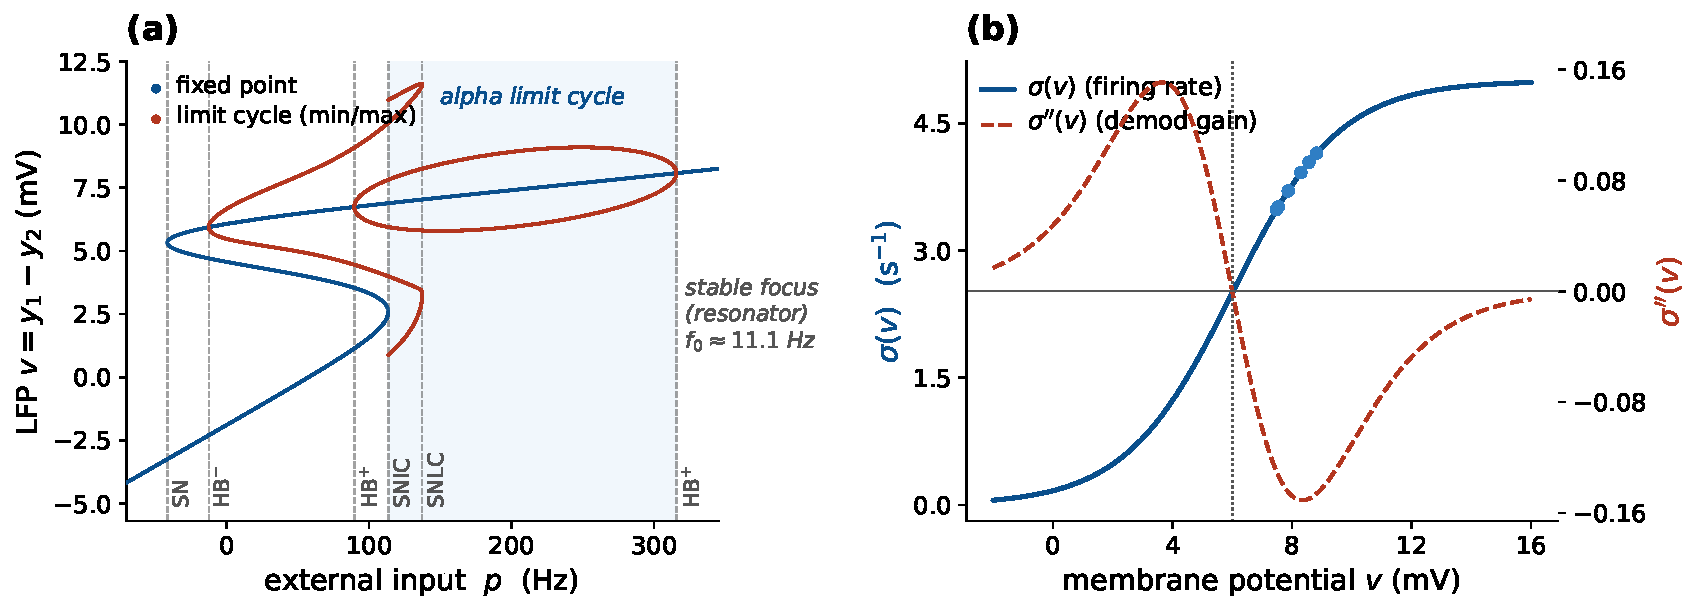
\includegraphics[width=\textwidth]{fig_bifurcation_sigmoid.pdf}
\caption{\textbf{The Jansen--Rit operating regime: bifurcation and sigmoid curvature.}
\emph{(a)} JR bifurcation diagram from numerical continuation---the LFP $v=y_1-y_2$ along
the fixed-point branch (blue) and the min/max of the limit-cycle branches (red) vs.\
external input $p$, with \emph{solid} stable and \emph{faded} unstable. The alpha limit
cycle (shaded) is bounded by a saddle-node-on-invariant-circle (SNIC, $p\!\approx\!114$)
and the supercritical Hopf ($p\!\approx\!315$, $f_0\!\approx\!11.1$~Hz); beyond the Hopf the
fixed point is a stable focus---the near-critical resonator regime used throughout. The
column is a weakly-damped focus near \emph{both} bifurcations, so it resonates on either
approach---more slowly near the SNIC. Further
codim-1 points are marked (saddle-node SN, Hopf HB$^{\pm}$, saddle-node of limit cycles
SNLC). \emph{(b)} The sigmoid $\Sig(v)$ and its curvature $\Sig''(v)$, which sets the
demodulation gain and vanishes at the inflection $v_0$. Dots mark the operating points
reached by the closed-loop model for the $p$ values used here.}
\label{fig:bif}
\end{figure}

The response at the envelope frequency is read out with a software lock-in
amplifier referenced to $\Omega$---a standard way to isolate the component of a signal
at one chosen frequency: multiply by sine and cosine at $\Omega$ and average, so
everything \emph{not} at $\Omega$ cancels and only the envelope-locked amplitude
survives. Concretely we multiply $v(t)$ by quadrature references and
integrate over a Hann-windowed measurement window to obtain the in-phase ($I$) and
quadrature ($Q$) components,
\begin{equation}
I=\frac{2}{\sum_k w_k}\sum_k w_k\,(v_k-\bar v)\cos\Omega t_k,\quad
Q=\frac{2}{\sum_k w_k}\sum_k w_k\,(v_k-\bar v)\sin\Omega t_k,\quad
A_\Omega=\sqrt{I^2+Q^2},
\label{eq:lockin}
\end{equation}
with $w$ a Hann window and $\bar v=\sum_k w_k v_k/\sum_k w_k$ the windowed mean.
For a pure tone $v=A\cos(\Omega t+\phi)$ the product-to-sum identity gives
$I\to A\cos\phi$ and $Q\to -A\sin\phi$, so $A_\Omega\to A$ exactly---the factor
$2/\sum_k w_k$ is the normalization that returns the physical amplitude, and
$A_\Omega$ equals twice the magnitude of the windowed Fourier coefficient at
$\Omega$. The one subtlety is that out-of-band components must not leak into the
estimate; the dangerous one is the DC level of $v$ ($\bar v\!\sim\!8$~mV, far
larger than the demodulated signal). Over an exact integer number of
$\Omega$-periods $\sum_k w_k\cos\Omega t_k=0$ and there is no leakage, but in
general it is nonzero, so we subtract $\bar v$ explicitly; this makes the metric
exact for a tone and robust down to the $10^{-8}$ level needed for the kHz
analysis (\S\ref{sec:khz}). The signed in-phase component $I$ alone recovers
$\half\Sig''(v^*)\varepsilon^2 m$ including its sign, which we use to verify the
curvature law (Fig.~\ref{fig:opp}).

Three auxiliary constructions support the main results. Throughout we contrast the
\emph{open-loop detector}---the firing-rate sigmoid alone at a fixed operating point
$v^*$, with no recurrence---against the \emph{closed-loop} column, the full recurrent
Jansen--Rit with its feedback. The open-loop detector passes the two-tone field through
$\Sig$ at $v^*$ and applies Eq.~\eqref{eq:lockin}, isolating the pure demodulation law
(Figs.~\ref{fig:carrier},~\ref{fig:opp},~\ref{fig:khz}). The \emph{bifurcation
diagram} records the field-free min/max of $v$ vs.\ $p$, each run initialized at
its fixed point plus a small kick. The \emph{two-dimensional map} evaluates
$A_\Omega$ over an ($\Omega,p$) grid. We verify the mechanism three ways: the
square law ($A_\Omega$ vs.\ $\varepsilon$ on a well-damped focus, expecting a
log--log slope of $2$); a linearization control (replacing $\Sig$ in
Eq.~\eqref{eq:jr0} by its tangent at $v^*$, which must abolish the $\Omega$
response); and a check of $\Sig',\Sig''$ against finite differences. All code is
openly available (see \emph{Code and data availability}).

\subsection{Laminar two-band model (LaNMM)}
We complement the single-column analysis with simulations of the laminar neural
mass model (LaNMM) of \S\ref{sec:nmm}. We integrate the full 28-variable column
\cite{ruffini2025cfc,sanchezTodo2023}, with the field entering exactly as in the single
JR column---as a membrane polarization added inside the sigmoid argument of the target
population,
\begin{equation}
\varphi_X(t)=\Sig\!\big(v_X(t)+s(t)\big),\qquad X\in\{P_1,P_2\},
\label{eq:lanmm_drive}
\end{equation}
with $s(t)$ the AM or two-tone field of \S\ref{sec:coupling} (amplitude $\varepsilon$ in
mV, beat $\Omega=2\pi\Delta f$, carrier $\omega_c=2\pi f_c$) and all three external drives
held flat at their baselines (Fig.~\ref{fig:lanmm_setup}). Coupling the field this way,
rather than as a perturbation of an external input \emph{rate}, matters for more than
tidiness: a rate cannot go negative, so a rate-coupled AM drive must be clipped at zero
once its excursion exceeds the baseline, and a hard clip is a half-wave rectifier---a
diode detector placed upstream of the sigmoid, which would inject a line at $\Delta f$
into the drive before the population nonlinearity ever saw it. A signed membrane
polarization carries no such constraint and none is applied. Because the LaNMM and JR
sigmoids share the voltage scale $1/\rho\approx1.8$~mV, $\varepsilon$ is directly
comparable between the two models. Integration is a vectorized fixed-step RK4
($\Delta t=10^{-4}$~s) advancing the whole parameter grid simultaneously, as in the JR
sweeps. In place of the lock-in (Eq.~\eqref{eq:lockin}) we read the
alpha-band ($8$--$12$~Hz) power of the $P_1$ and $P_2$ membrane potentials from the
Hilbert envelope over a post-transient window---a phase-robust measure suited to
the entrainment regime, where lock-in phase slips would otherwise complicate the
read-out. Two sweeps probe the column: an amplitude--beat sweep over
$(A,\Delta f)$ at fixed carrier (the Arnold tongue), and a carrier--beat sweep over
$(f_c,\Delta f)$ at fixed $A$, built on the LaNMM module of \cite{ruffini2025cfc}. The maps
(Figs.~\ref{fig:lanmm_p2},~\ref{fig:lanmm_p1}) show the \emph{stimulation-induced} alpha
enhancement, alpha power minus the unstimulated ($A=0$, no modulation) baseline, which
removes the per-simulation offset so the resonant structure is visible. For the
alpha resonance we instead drive the deep $P_1$ loop directly and sweep its input against
$\Delta f$, reading the lock-in (Eq.~\eqref{eq:lockin}) of $v_{P_1}$ at $\Delta f$.

\subsection{Exact next-generation mean field (NMM2 PING)}
We test the mechanism in the exact next-generation mean field (NMM2, \S\ref{sec:nmm}),
following the Rosetta Stone formulation of \cite{ruffini2025rosetta} (which places the
Montbri\'o--Paz\'o--Roxin reduction \cite{montbrio2015} on a common footing with the JR
and LaNMM models used here), where the firing-rate nonlinearity is the derived MPR
dynamics of Eq.~\eqref{eq:mpr} rather than a postulated sigmoid. We use a two-population
excitatory--inhibitory (PING) motif \cite{ruffini2021nmm2,clusella2023,ruffini2025rosetta}:
each population $\alpha\in\{E,I\}$ is an MPR mean field (firing rate $r_\alpha$, mean
potential $v_\alpha$) with membrane time $\tau_\alpha$, coupled through second-order
synapses,
\begin{equation}
\begin{aligned}
\tau_E\dot r_E&=\Delta/(\pi\tau_E)+2r_Ev_E, &\quad
\tau_E\dot v_E&=v_E^2+\bar\eta-(\pi\tau_E r_E)^2+\tau_E C\,(s_E-s_I)+\delta V(t),\\[2pt]
\tau_I\dot r_I&=\Delta/(\pi\tau_I)+2r_Iv_I, &\quad
\tau_I\dot v_I&=v_I^2+\bar\eta-(\pi\tau_I r_I)^2+\tau_I C\,(s_E-2s_I),
\end{aligned}
\label{eq:nmm2-ping}
\end{equation}
with second-order synaptic activations $s_E=\hat K_a[r_E]$ (excitatory, time constant
$\tau_a$) and $s_I=\hat K_g[r_I]$ (inhibitory, $\tau_g$), each obeying the same
critically-damped operator as the JR synapse, $\tau^2\ddot s+2\tau\dot s+s=r$; here $C$
is the global synaptic gain and the weights $(A_{ee},A_{ei},A_{ie},A_{ii})=(1,1,1,2)$
set the E and I rows---i.e.\ the $E$ membrane sees $C\,(s_E-s_I)$ and the $I$ membrane
$C\,(s_E-2s_I)$, the only asymmetry being the doubled $I\!\to\!I$ weight $A_{ii}=2$. The common background drive $\bar\eta$---the same in both
populations, with no separate input current---is the bifurcation parameter: raising it
past a supercritical Hopf at $\bar\eta\!\approx\!1$ opens a gamma limit cycle (the gamma
counterpart of the JR alpha Hopf). The applied field enters the excitatory membrane
current as $\delta V(t)=\lambda E(t)$ as two genuine tones at $f_c\mp\Delta f/2$ (carrier
$f_c=300$~Hz, envelope $\Delta f$ swept through the gamma band); the polarization is
expressed in the dimensionless MPR units of $v_E$, so the carrier is
rectified by the exact quadratic $v_E^2$ term, with no postulated sigmoid. We
integrate with fixed-step RK4 ($\Delta t=0.05$~ms) and read out the lock-in
(Eq.~\eqref{eq:lockin}) of $r_E$ at $\Delta f$ over the $(\Delta f, \bar\eta)$ plane.
Parameters (Rosetta Stone PING \cite{ruffini2025rosetta}): $\Delta=1$, global coupling
$C=15$, $\tau_E=15$, $\tau_I=7.5$, $\tau_a=10$, $\tau_g=2.5$~ms, with $\bar\eta$ swept
through the supercritical Hopf at $\bar\eta\!\approx\!1$ ($f_0\!\approx\!55$~Hz).

Two parameters reach this gamma Hopf, and we use both as criticality knobs---just as the
external drive $p$ and the coupling $C$ both reach the JR alpha Hopf. The background drive
$\bar\eta$ (above) is swept for the resonance map (Fig.~\ref{fig:nmm2_map}); the global
coupling $C\,(\equiv J)$ is swept for the J-curve (Fig.~\ref{fig:nmm2_jcurve}): we vary
$J$ at fixed $\bar\eta$ toward the gamma Hopf $J^*$ (located by bisection on the leading
Jacobian eigenvalue) and read the lock-in peak of $r_E$ over $\Delta f$. Unlike the JR
J-curve, \emph{no operating-point pinning is needed}, because here the rectifier is the
exact $v_E^2$ term, whose quadratic coefficient is fixed by construction; sweeping $J$
therefore changes only the damping $\gamma$, isolating the amplification cleanly.

\subsection{QIF spiking network (microscale of NMM2)}\label{sec:qif-methods}
NMM2 is the exact mean field of an all-to-all network of QIF neurons
\cite{montbrio2015,ruffini2025rosetta,clusella2023}, so we integrate that network directly
to test the prediction at the spike level (\S\ref{sec:qif}): $N=8000$ QIF neurons per
population, parameters identical to the PING mean field (Eq.~\eqref{eq:nmm2-ping}),
excitabilities $\eta_j\sim$ Lorentzian$(\bar\eta,\Delta)$ sampled by deterministic
quantiles, second-order synapses driven by the empirical population rates, and a genuine
two-tone field entering the excitatory membranes. Spiking and threshold dynamics are
where the AM surrogate and the physical waveform cannot be assumed equivalent beyond
perturbation theory, so this run uses two tones throughout. The bifurcation parameter is the common
background drive $\bar\eta$, with a gamma Hopf at $\bar\eta_{\rm Hopf}\!\approx\!1.1$
(autonomous $f_0\!\approx\!53$~Hz; these finite-$N$ values sit just above the exact
mean-field Hopf $\bar\eta\!\approx\!1$, $f_0\!\approx\!55$~Hz, the small offset being a
finite-size effect); the carrier is $f_c=300$~Hz and the field amplitude $A_f=35$. Because
this is a \emph{gamma} circuit, the TI beat $\Delta f$ is set in the gamma band:
$\Delta f=55$~Hz \emph{near} the forced gamma resonance ($\bar\eta=0.85$, below the Hopf) and
$\Delta f=42$~Hz in the oscillatory regime ($\bar\eta=1.5$, above the Hopf)---a detuning of
$\approx$11~Hz below the autonomous $f_0\!\approx\!53$~Hz that places the beat outside the
$1{:}1$ Arnold tongue, so the above-Hopf response is gating, not entrainment
(\S\ref{sec:vocab}). Envelope-locked timing is quantified by the quadrature lock-in
$A_\Omega$ of $r_E(t)$ at $\Delta f$, reported as the modulation depth
$A_\Omega/\langle r_E\rangle$ (a stable measure---the off$\to$on lock-in ratio would divide
by the near-zero field-free baseline).

\subsection{Coupling sweeps, timing, and the tACS control (Jansen--Rit)}
The coupling sweeps of Figs.~\ref{fig:jcurve} and~\ref{fig:timing}, and the transcranial
alternating-current stimulation (tACS) control of Fig.~\ref{fig:tacs}, use the single JR
column with the operating point $v^*$ pinned: for
each global connectivity $C$ we solve the field-free fixed-point relation analytically
for the external drive $p(C)$ that holds $v^*$ (hence $\Sig''(v^*)$) fixed, vary $C\,(=J)$
toward the alpha Hopf, and read $\gamma,\omega_0$ from the $6\times6$ Jacobian. The field
is the AM drive of Eq.~\eqref{eq:am} for TI (Fig.~\ref{fig:jcurve}; AC lock-in vs DC mean
rate for Fig.~\ref{fig:timing}) or a direct in-band sinusoid $s(t)=\varepsilon\cos\Omega t$
($\varepsilon=0.1$~mV) for the tACS control (Fig.~\ref{fig:tacs}), each read out by the
lock-in of $v$ at $\Delta f$.

\subsection{Vocabulary: forced response, entrainment, and gating}
``Entrainment'' is used in several senses, so we fix three terms. \emph{Forced response}
is the driven, non-autonomous case below the Hopf, quantified by the lock-in amplitude at
the beat $\Delta f$ (Eq.~\eqref{eq:lockin}). \emph{Entrainment} is reserved for its
dynamical-systems meaning, frequency capture of a \emph{self-sustained} oscillator, tested
by the $1{:}1$ criterion $|f_{\rm out}-\Delta f|<0.3$~Hz on the dominant output frequency
\cite{pikovsky2001}. \emph{Gating} is amplitude modulation of a persisting rhythm without
frequency capture \cite{canolty2010,tort2010}. The distinction is load-bearing, since
capture and gating are dynamically different and the same word would otherwise cover both;
Appendix~\ref{sec:vocab} gives the metrics and the Arnold-tongue protocol.

\section{Results}
We present the evidence on three rungs of the modeling ladder: the single
Jansen--Rit column (closed form, analyzable), the laminar LaNMM (two native
resonances and genuine carrier dependence), and the exact next-generation mean
field (NMM2, the demodulating nonlinearity derived rather than postulated). Each
rung shows the same pair---square-law demodulation followed by near-Hopf
amplification. Two mesoscale signatures then follow that have no single-cell analog:
the network's own coupling sets the gain at fixed detection (the $J$-curve,
\S\ref{sec:jcurve}), and the resonance amplifies oscillatory \emph{timing} far more than
mean \emph{rate} (\S\ref{sec:timing})---the spiking-level prediction we test in the QIF
network.

\subsection{The Jansen--Rit sigmoid demodulates: an alpha line from a carrier-only input}
The system is oriented by Fig.~\ref{fig:bif}: a clean supercritical Hopf at
$p\!\approx\!315$ with $f_0\!\approx\!11.1$~Hz, and a sigmoid whose curvature peaks
well off the inflection, so the closed-loop operating points sit where $\Sig''$ is
large. The core result is Fig.~\ref{fig:demod}: an input with no spectral power in
the alpha band (lines only at $f_c$ and $f_c\pm\Delta f$) produces a clean
$\sim$11~Hz output oscillation locked to the envelope, with a strong alpha peak in
the output spectrum absent from the input.

\begin{figure}[t!]
\centering
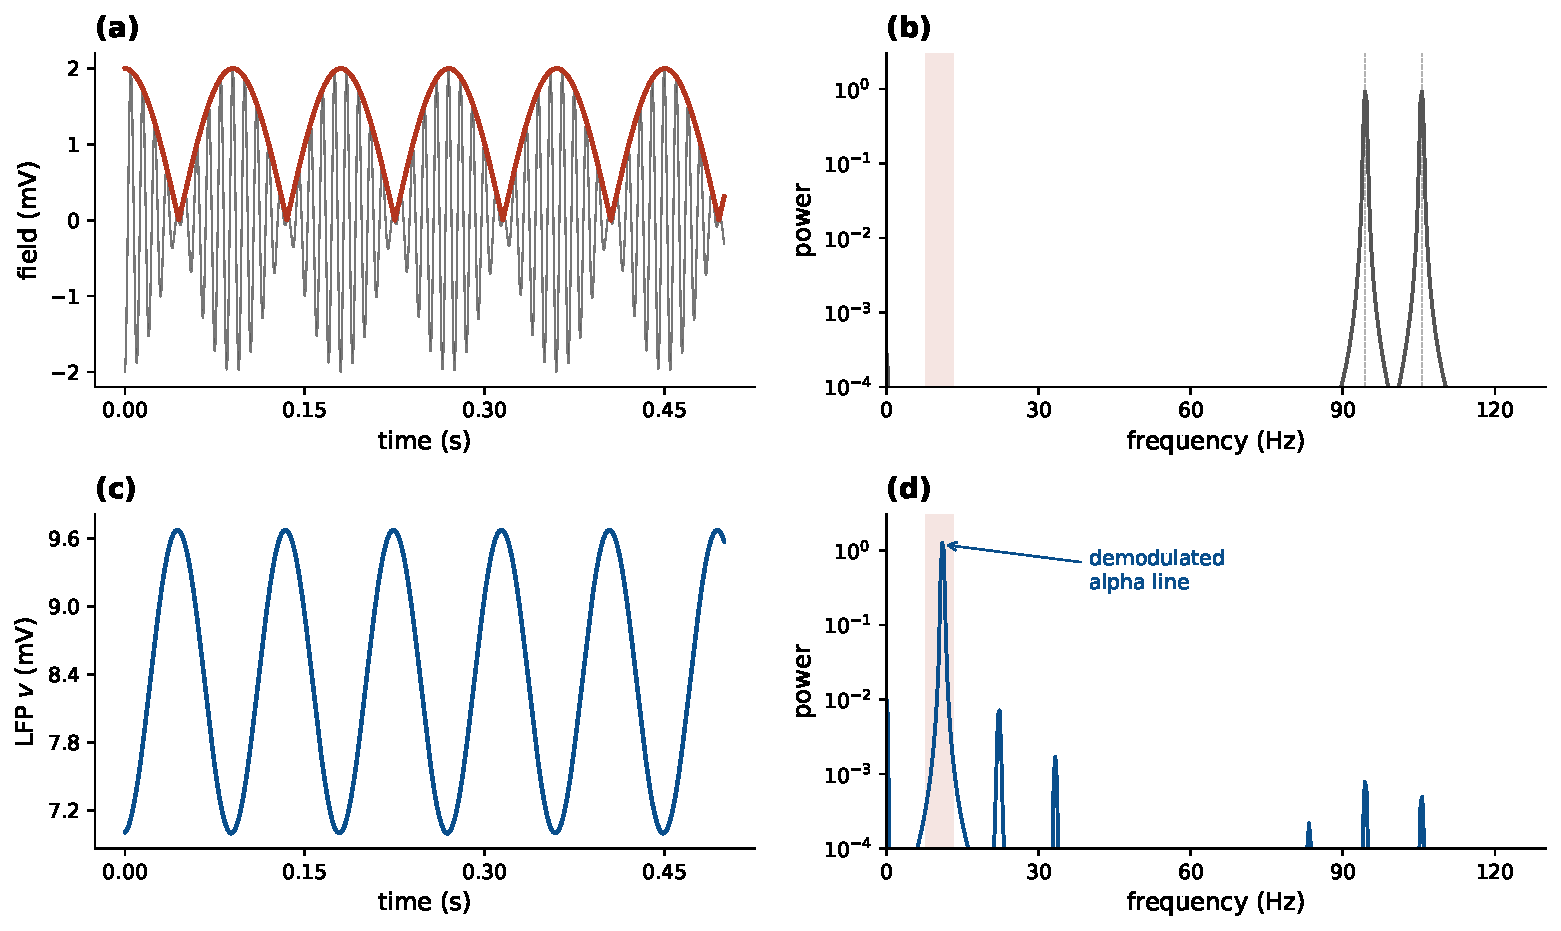
\includegraphics[width=\textwidth]{fig_demodulation_twotone.pdf}
\caption{\textbf{An alpha rhythm is synthesized from a two-tone TI input (Jansen--Rit
below Hopf).} The field is the physical TI waveform, two equal tones at
$f_{1,2}=f_c\mp\Delta f/2$, not the amplitude-modulated surrogate. \emph{(a)} The field
$s(t)$ and its envelope $A(t)=2\varepsilon|\cos(\Omega t/2)|$---a rectified cosine, not a
sinusoid; it is $A^2$ that is sinusoidal at $\Omega$ (\S\ref{sec:coupling}).
\emph{(b)} The input spectrum has lines only at $f_1$ and $f_2$ ($94.5$ and $105.6$~Hz)
and no third line at the carrier; power in the alpha band (shaded) is
$1.6\times10^{-8}$, i.e.\ empty to numerical precision.
\emph{(c)} The output $v=y_1-y_2$ oscillates at the envelope frequency.
\emph{(d)} The output spectrum has a strong peak at $\Omega=11.0$~Hz,
synthesized by the sigmoid and absent from the input.}
\label{fig:demod}
\end{figure}

\subsection{Near the Hopf, the demodulated beat drives a sharp resonance}
The resonance is quantified in Fig.~\ref{fig:res}. In the
fixed-point regime ($p>315$, a stable focus) the response is a Lorentzian centered at
$f_0$ whose height grows monotonically as the Hopf is approached
($0.23\!\to\!0.43\!\to\!0.70$~mV; Fig.~\ref{fig:res}), i.e.\ gain $\propto1/\gamma$. This
is genuine forced gain: with no drive the focus is silent at $\Omega$, so all power at
$\Omega$ is synthesized by the demodulating nonlinearity and amplified by the recurrent
loop. Above the Hopf ($p<315$) the
column free-runs at $f_0$ and the demodulated drive instead phase-locks that autonomous
alpha within a $1{:}1$ Arnold tongue; because lock-in amplitude at $\Omega$ then conflates
the driven response with the free-running cycle, we characterize that regime with the
output frequency $f_{\rm out}$ rather than the lock-in amplitude (Fig.~\ref{fig:entrain}).

\begin{figure}[t!]
\centering
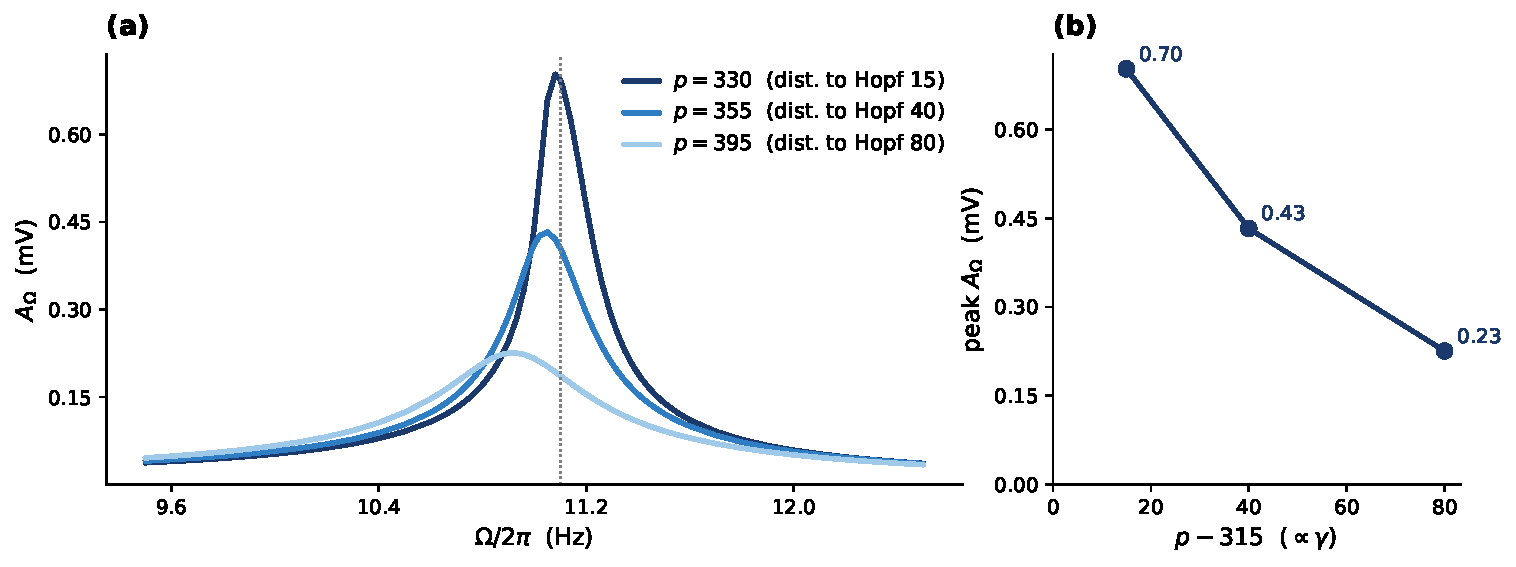
\includegraphics[width=\textwidth]{fig_resonance.pdf}
\caption{\textbf{The demodulated beat drives a resonance that sharpens toward the Hopf (Jansen--Rit).}
Fixed-point regime ($p>315$, stable focus): lock-in response at $\Omega$ vs.\ envelope
frequency ($\varepsilon=0.3$~mV). \emph{(a)} The demodulated drive forces a Lorentzian
resonance at $f_0\!\approx\!11.1$~Hz whose peak redshifts slightly as the damping grows
($\omega_{\rm peak}=\sqrt{\omega_0^2-2\gamma^2}$; $11.08\!\to\!10.93$~Hz across the three
curves); the response carries no power at $\Omega$ in the absence of drive, so this is
genuine forced gain. \emph{(b)} The peak height grows as the Hopf is
approached ($p\!\to\!315$, distance to Hopf $\to0$). Three points cannot establish a power
law; the $1/\gamma$ scaling is quantified over a decade, together with its saturation, in
Fig.~\ref{fig:jcurve}(c). The complementary above-Hopf regime, where the demodulated drive
\emph{entrains} the autonomous alpha within a $1{:}1$ Arnold tongue, is characterized with
the appropriate observable (output frequency $f_{\rm out}$, not lock-in amplitude) in
Fig.~\ref{fig:entrain}.}
\label{fig:res}
\end{figure}

\subsection{Carrier independence and the kHz roll-off}
At fixed post-coupling polarization the demodulated response is flat across the
carrier band, for both the open-loop detector and the closed-loop column near the Hopf
(Fig.~\ref{fig:carrier}). As a function of
the \emph{applied} field, by contrast, the membrane low-pass makes the response roll
off as $1/f_c^2$ above the corner (Fig.~\ref{fig:khz}): passive somatic demodulation
is suppressed four to six orders of magnitude at kHz, whereas a fast element
($\tau\!\approx\!0.2$~ms) retains an appreciable response into the kHz band.

\begin{figure}[t!]
\centering
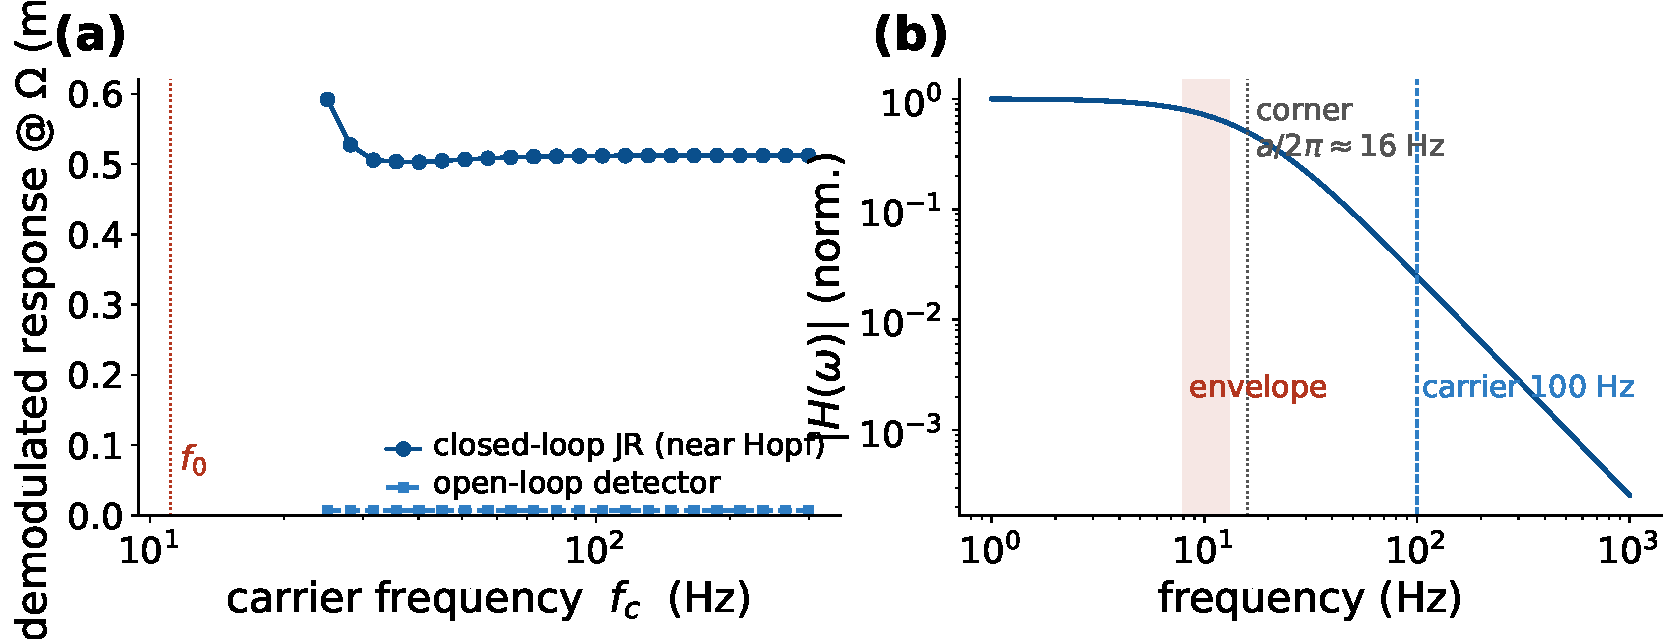
\includegraphics[width=\textwidth]{fig_carrier_independence.pdf}
\caption{\textbf{The demodulated response is carrier-independent at fixed polarization (Jansen--Rit).} \emph{(a)} The demodulated response is
flat across carrier frequency $f_c=25$--$300$~Hz, both for the open-loop detector
(exactly, by Eq.~\eqref{eq:demod}) and for the closed-loop JR near the Hopf (which
adds $\sim$60$\times$ resonant gain); deviations appear only as $f_c$ approaches
the natural band. \emph{(b)} The second-order-synapse band-pass $|H(\omega)|$
passes the envelope ($\sim$0.7) and suppresses the $100$~Hz carrier ($\sim$2.5\%). Dotted line: synaptic corner $a/2\pi\!\approx\!16$~Hz; shaded band: envelope ($8$--$13$~Hz); dashed line: $100$~Hz carrier.}
\label{fig:carrier}
\end{figure}

To pre-empt the objection that the demonstration runs only at $100$~Hz, we drive the
full recurrent column with a genuine kHz field, passing it through
an explicit membrane low-pass (an extra first-order state, time constant $\tau$) for
each coupling route before it reaches the sigmoid (Fig.~\ref{fig:khz_direct}a). The
column demodulates and resonates at the recovered alpha well into the kHz band when
the nonlinearity sits at a fast element ($\tau\!\approx\!0.2$~ms), exactly as
Eq.~\eqref{eq:khz} predicts (Fig.~\ref{fig:khz_direct}a). Driving the fast-element route
with two \emph{genuine} tones at $f_{1,2}=1994.5$ and $2005.5$~Hz---a real TI waveform at
a real TI carrier, beating at $10.9$~Hz---the input carries $2.2\times10^{-13}$ of power
in the $8$--$14$~Hz band, i.e.\ none, while the output carries a clean line at $11.0$~Hz
(Fig.~\ref{fig:khz_twotone}), with the attenuation set by the analytic
$|H_m|^2\!=\!0.137$ at $2$~kHz for $\tau=0.2$~ms. The kHz claim therefore rests on the
physical waveform, not on an extrapolation from the AM surrogate. That the bare unmodulated kHz carrier is itself
weakly effective---the premise of TI's focality---is consistent with the limited
sensitivity of hippocampal network oscillations to unmodulated kHz fields
\cite{esmaeilpour2020}.

\subsection{The nonlinearity is the detector: the
\texorpdfstring{$\Sig''$}{sigma''} curvature law and its controls}\label{sec:results-curvature}
The signed open-loop response tracks $\half\Sig''(v^*)\varepsilon^2 m$ across the
operating range, vanishing and reversing sign at the inflection $v_0$
(Fig.~\ref{fig:opp})---demodulation is the sigmoid-curvature term of
Eq.~\eqref{eq:demod}, and the closed-loop operating points sit where $\Sig''$ is large
and negative.

\begin{figure}[t!]
\centering
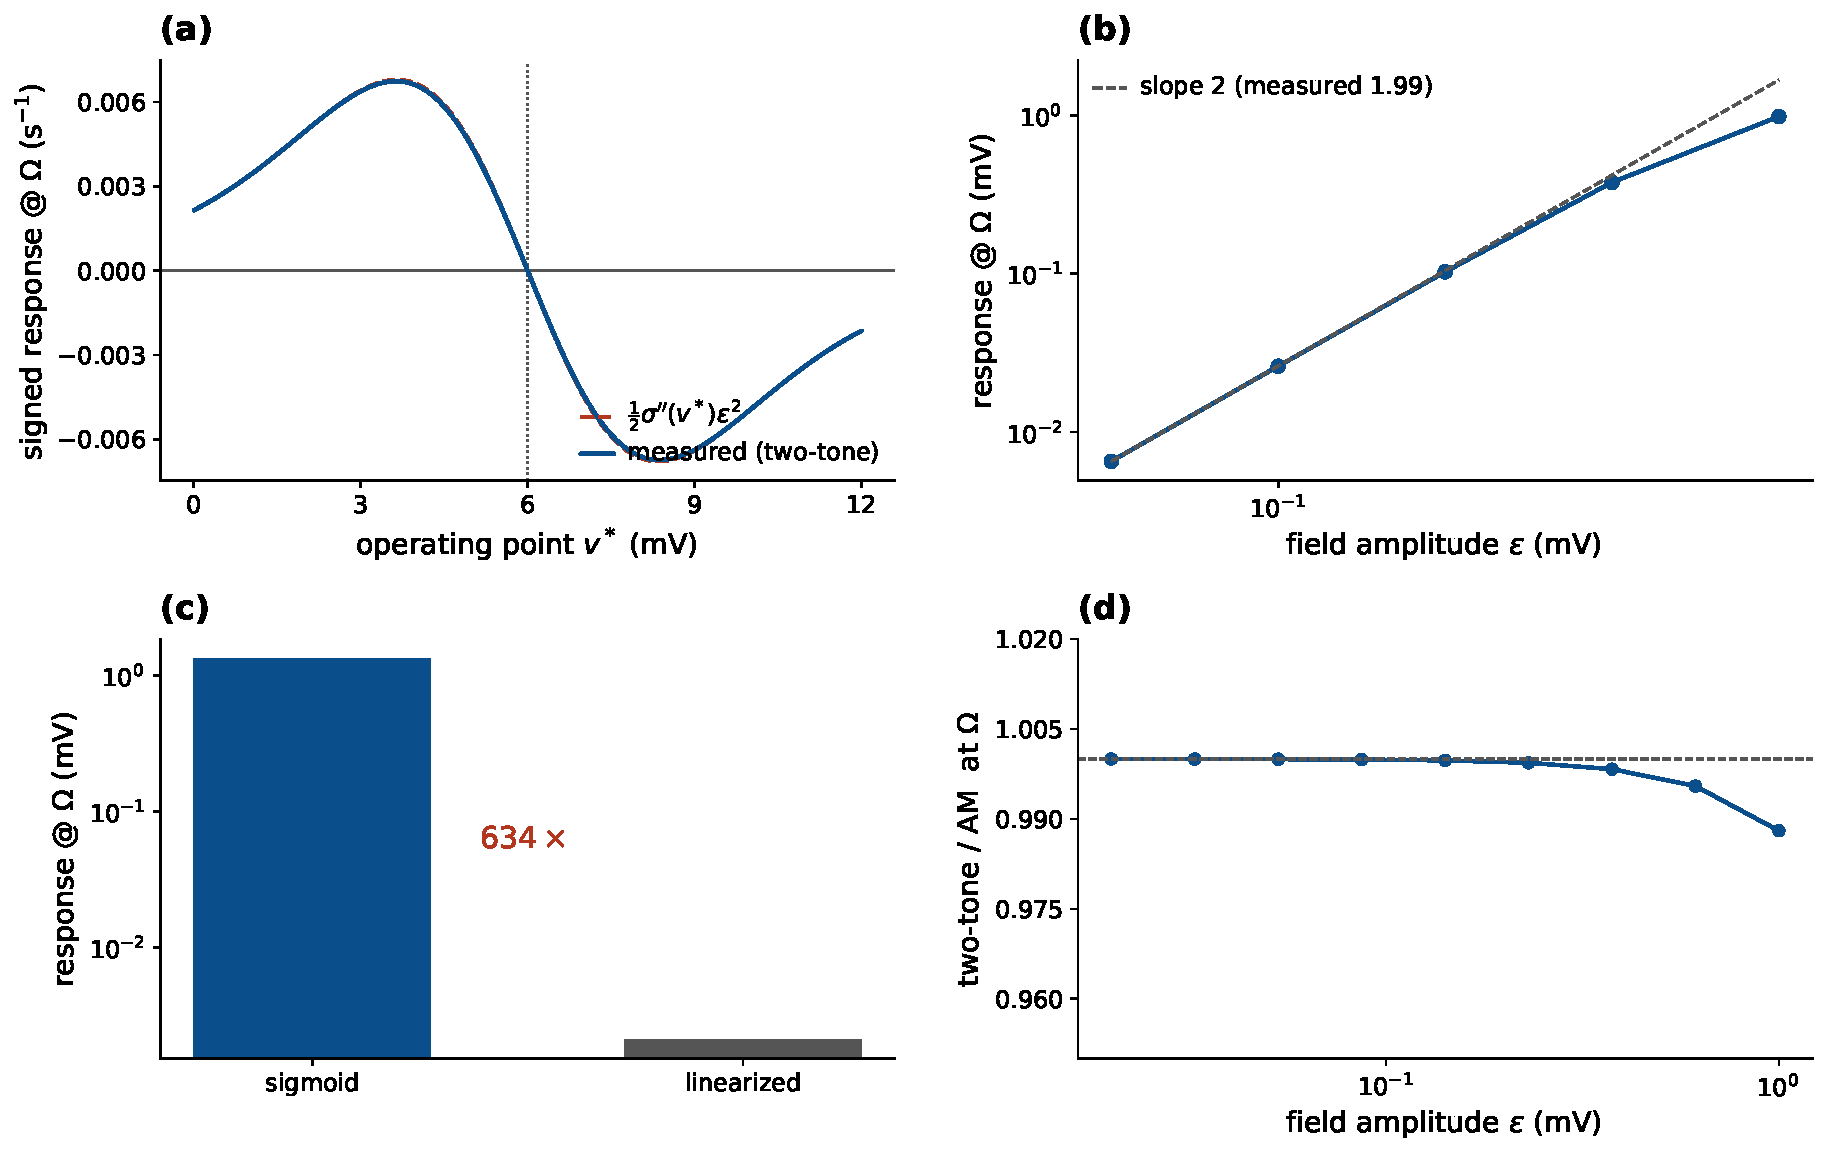
\includegraphics[width=\textwidth]{fig_curvature_twotone.pdf}
\caption{\textbf{The curvature law, the square law, and the surrogate control
(Jansen--Rit, genuine two tones).} \emph{(a)} The signed open-loop response tracks
$\half\Sig''(v^*)\varepsilon^2$ across the operating range (maximum deviation $0.9\%$),
vanishing at the inflection $v_0$ and reversing sign across it. The mechanism is
sign-agnostic: $\Sig''$ sets sign and phase while $|\Sig''|$ sets gain, so the resonance
picture is unchanged up to an overall sign in the $\Sig''>0$ lobe, which this sweep spans.
The sign flip is itself a prediction (\S\ref{sec:predictions}). \emph{(b)} The closed-loop
response scales as $\varepsilon^2$, measured slope $1.99$. \emph{(c)} Replacing the
field-receiving sigmoid by its tangent collapses the response $634\times$. \emph{(d)}
Surrogate control: the two-tone/AM ratio at $\Omega$ approaches $1$ as
$\varepsilon\!\to\!0$ ($1.0000$ at $0.02$~mV, $0.988$ at $1$~mV), licensing the AM
surrogate for the dense sweeps of Fig.~\ref{fig:jcurve}, which read only that component,
and for nothing else.}
\label{fig:opp}
\end{figure}

Two controls close the argument (Fig.~\ref{fig:opp}b,c): the response scales as
$\varepsilon^2$ at small drive (measured log--log slope $1.99$ against the
predicted $2$), and replacing the field-receiving sigmoid by its linearization
collapses the response by $634\times$ ($1.34\!\to\!0.0021$~mV)---the nonlinearity is
the detector, and its curvature is the gain. A third panel settles the surrogate
question: at matched amplitude the two-tone and AM responses at $\Omega$ agree to
within $10^{-4}$ at $\varepsilon=0.02$~mV and to $1.2\%$ at $1$~mV
(Fig.~\ref{fig:opp}d), so the dense perturbative sweeps below, which read only the
$\Omega$ component, may use either waveform.

\subsection{Two native resonances and nonlinear Arnold tongues in the LaNMM}\label{sec:lanmm-results}
The single JR column isolates and lets us analyze the mechanism; the laminar model
(LaNMM, \S\ref{sec:nmm}) confirms it in a cortical column with its \emph{own} two
resonances. Driving one population with the two-tone field of Eq.~\eqref{eq:lanmm_drive}
and reading the alpha-band power of the deep ($P_1$, alpha) and superficial ($P_2$,
gamma) pyramidal potentials (Methods, Fig.~\ref{fig:lanmm_setup}), we recover the
same envelope resonance, now carrying the column's intrinsic rhythms.

Driving the deep $P_1$ (alpha) loop directly and sweeping the envelope frequency
$\Delta f$ reproduces the single-column picture in the laminar model
. With the $P_1$ input as the
bifurcation parameter, the stable-focus side (high drive) gives a forced alpha
resonance at $\sim$10~Hz that grows as the alpha Hopf is approached, while the
limit-cycle side (low drive) entrains the autonomous alpha---the same
stable-focus/limit-cycle pair as the JR column (Fig.~\ref{fig:res}), now read out as
the deep-pyramidal alpha lock-in. The heuristic laminar model thus shows the JR
resonance \emph{and}, in addition, the carrier-dependent Arnold tongues that follow.

One qualification governs the laminar sweeps. They run to $\varepsilon=3$~mV on $P_2$,
above the sigmoid voltage scale $1/\rho\approx1.8$~mV, so they sit deliberately in a
nonlinear, non-perturbative regime. They are a demonstration of tongues and frequency
capture, not a verification of the weak-field square law; that verification is the
low-amplitude JR and NMM2 work (Fig.~\ref{fig:opp}b), which stays two orders of magnitude
below $1/\rho$.

Sweeping the field amplitude $\varepsilon$ and beat frequency $\Delta f$ at a fixed
carrier produces \emph{nonlinear Arnold tongues}: alpha power in $P_1$ is maximal
when $\Delta f$ matches the deep alpha ($\sim$10~Hz) and grows with $\varepsilon$
(Figs.~\ref{fig:lanmm_p2}a,b and~\ref{fig:lanmm_p1}a,b)---envelope resonance and
phase locking of the slow generator to the recovered beat component, exactly as in the
JR resonance curves but now in a biophysical two-band column.

The carrier dependence reproduces, and physically grounds, the two coupling
limits of \S\ref{sec:coupling}--\S\ref{sec:khz}. Sweeping carrier $f_c$ against
beat $\Delta f$: when the field is delivered to the \emph{superficial} loop
($P_2$), strong $P_1$ demodulation requires a \emph{double} resonance---$f_c$ near
the $P_2$ gamma ($\approx$44~Hz) \emph{and} $\Delta f$ near the $P_1$ alpha
($\approx$10~Hz) (Fig.~\ref{fig:lanmm_p2}c,d): the fast loop acts as a tuned
``RF front end'' that must itself be excited before it can pass a demodulated
envelope to $P_1$, and off that gamma resonance the response collapses to
$\sim$7\% of its peak. When the field is delivered \emph{directly} to the slow
generator ($P_1$), the picture inverts: the envelope-locked response persists at
every carrier from $25$ to $80$~Hz, falling only to $\sim$25\% of its peak, and the
ridge sits at $\Delta f\!\approx\!10.5$~Hz even for a $60$~Hz carrier
(Fig.~\ref{fig:lanmm_p1}c)---broadband in $f_c$, as Eq.~\eqref{eq:demod} predicts for
direct coupling. This contrast requires the phase-sensitive read-out: because $P_1$
free-runs at its own alpha, band power alone buries a weak envelope-locked drive under
an autonomous rhythm that is not phase-locked to the beat, and only the lock-in at
$\Delta f$ separates the two (Methods). Real TI, in which the field
reaches deep generators through faster elements, sits between these limits: a
carrier matched to a fast (gamma) network resonance couples best, but the envelope
response persists---weaker---off resonance. This both confirms the JR mechanism
and refines it: the ``inert carrier'' of \S\ref{sec:carrier} is the
direct-coupling idealization, while a band-limited intermediary makes the carrier
choice matter, consistent with frequency-tagging/intermodulation paradigms
\cite{gordon2019}.

\begin{figure}[t!]
\centering
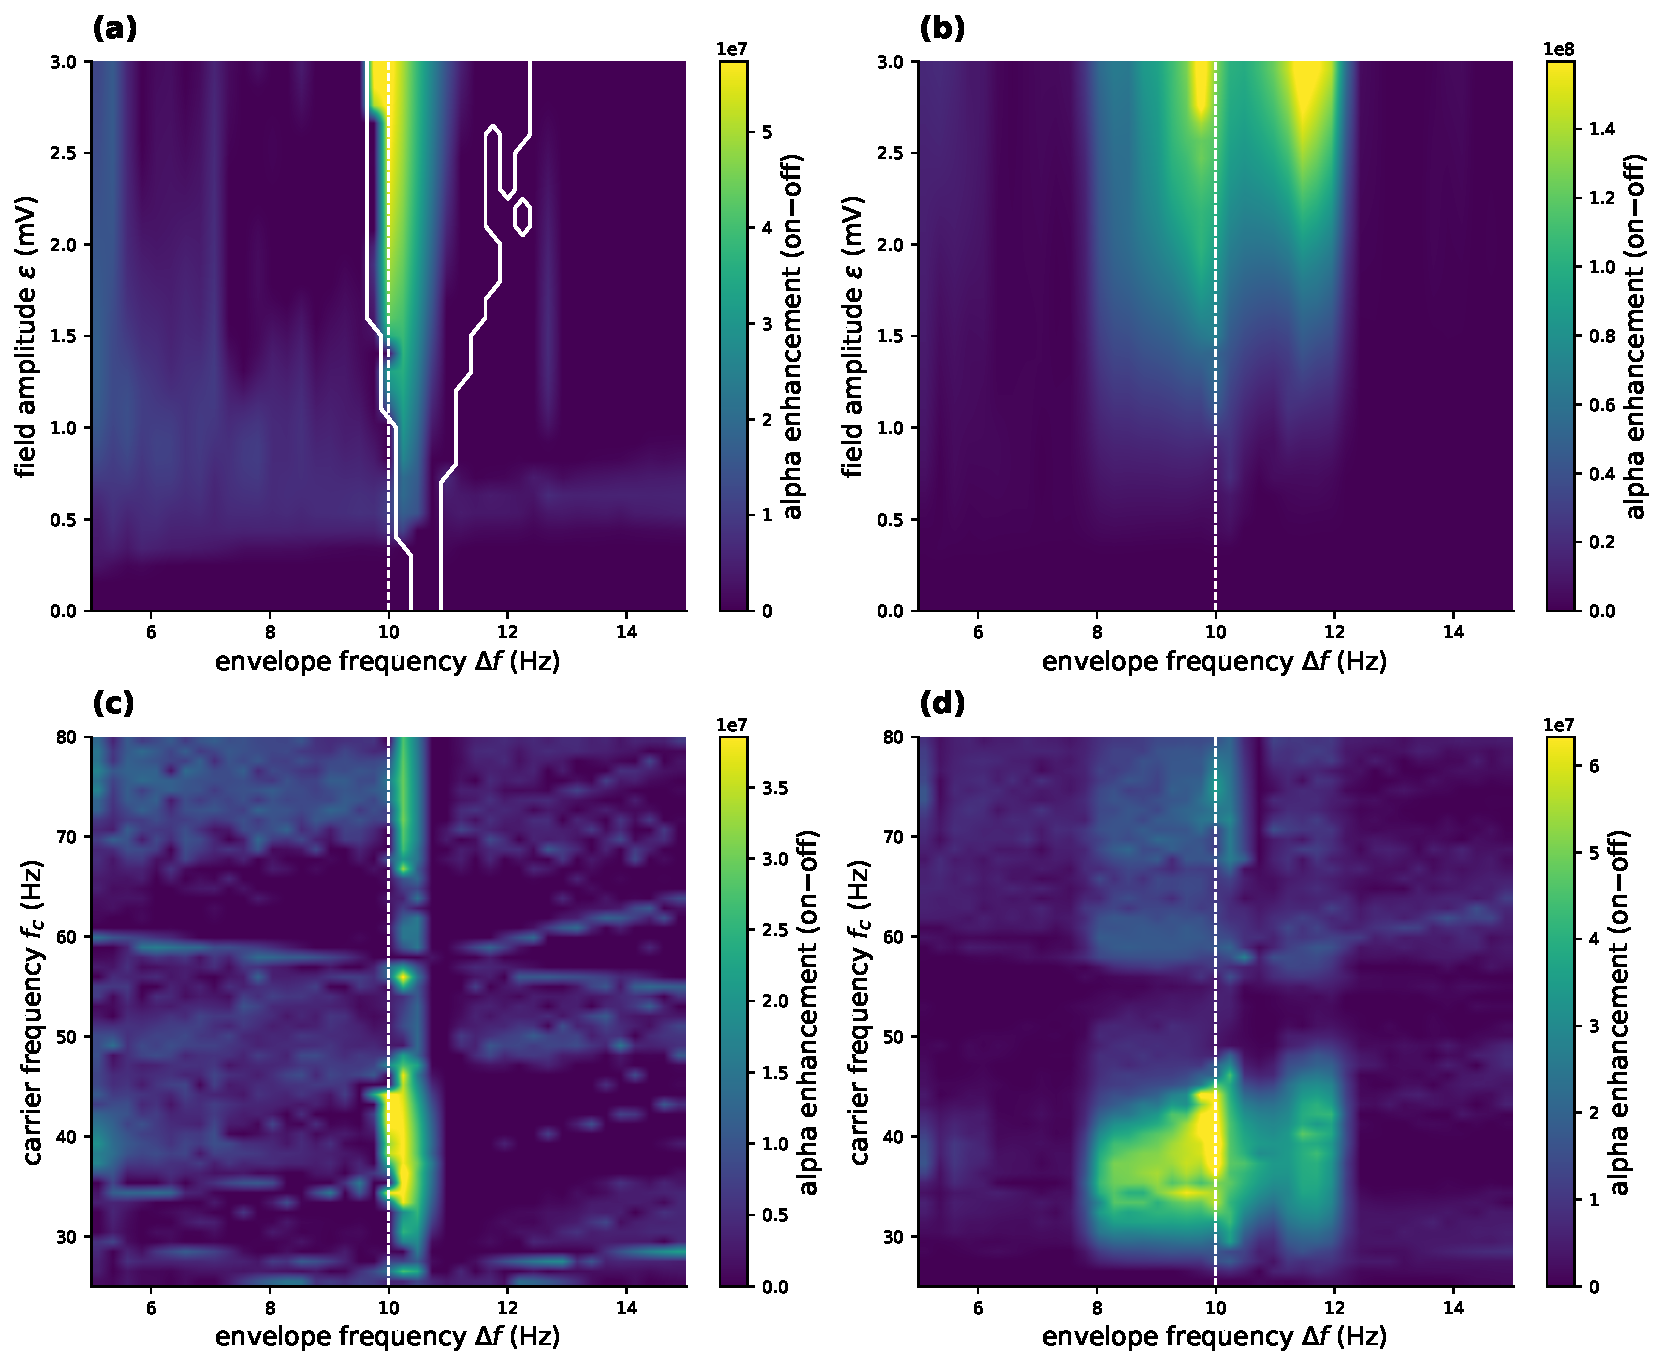
\includegraphics[width=0.86\textwidth]{fig_lanmm_field_p2_twotone.pdf}
\caption{\textbf{LaNMM Arnold tongues: two-tone TI field on the superficial $P_2$ (gamma)
loop.} The field enters the $P_2$ sigmoid argument as a membrane polarization $\varepsilon$
(mV) with all external drives flat. Color shows alpha-band ($8$--$12$~Hz) power minus the
unstimulated $\varepsilon=0$ baseline. \emph{(a,b)} $P_1$ and $P_2$ enhancement vs.\
$\varepsilon$ and $\Delta f$ (carrier $40$~Hz), peaking at the $P_1$ alpha ($10.0$~Hz,
dashed). The white contour in \emph{(a)} is the $1{:}1$ captured set
(Appendix~\ref{sec:vocab}), drawn explicitly because band power alone cannot separate
capture from a forced response; its width grows from $0.5$~Hz at $\varepsilon\!\to\!0$ to
$2.75$~Hz at $3$~mV. \emph{(c,d)} Enhancement vs.\ carrier and $\Delta f$ at
$\varepsilon=1.5$~mV: $P_1$ demodulation needs \emph{both} a carrier near the $P_2$ gamma
($\approx$$44$~Hz) and $\Delta f$ near the $P_1$ alpha---a double resonance.}
\label{fig:lanmm_p2}
\end{figure}

Concretely the LaNMM predicts that TI efficacy should (i) peak when $\Delta f$
matches a region's intrinsic alpha; (ii) widen and strengthen with modulation
amplitude (the tongue); and (iii) for fields delivered via superficial fast
circuits, be largest when the carrier is matched to a gamma network
resonance---e.g.\ two nearby gamma carriers summing to a $\sim$40~Hz-centered AM
field---while remaining present, weaker, for off-resonance carriers
\cite{esmaeilpour2021,violante2023}.

\subsection{Exact mean-field confirmation: the NMM2 PING gamma generator}\label{sec:nmm2-results}
The JR column and the LaNMM both use the heuristic firing-rate sigmoid (NMM1). As a
third, independent test we move to the exact next-generation mean field (NMM2,
Eq.~\eqref{eq:mpr}), where the demodulating nonlinearity is the \emph{derived}
quadratic $v^2$ term rather than a postulated curve. We drive the two-population E--I PING motif of
Eq.~\eqref{eq:nmm2-ping} (Methods)---a gamma generator that loses stability through
a supercritical Hopf (at $\bar\eta\!\approx\!1$, $f_0\!\sim\!55$~Hz), the gamma
counterpart of the JR alpha Hopf---with the two-tone field entering the excitatory current,
so the carrier is rectified by the exact $v_E^2$ term.

Driving with a two-tone TI field (carrier $f_c=300$~Hz, envelope $\Delta f$ swept through
the gamma band) and locking in the excitatory rate $r_E$ at $\Delta f$ reproduces the
whole picture (Figs.~\ref{fig:nmm2_res},~\ref{fig:nmm2_map}). Below the Hopf the
response is a forced resonance at the gamma frequency whose height grows as the
bifurcation is approached---the $1/\gamma$ gain of Eq.~\eqref{eq:gain}; above it the
demodulated drive entrains the autonomous gamma. The two-dimensional map traces a
ridge at $\Delta f\!\approx\!f_0$ that intensifies through the Hopf. Unlike the
static-sigmoid models, the resonant frequency itself \emph{shifts with the operating
point}---the ridge is diagonal, not vertical---a direct signature of the dynamic,
state-dependent transfer of the exact theory \cite{clusella2023}. That the same
demodulation-and-near-Hopf-resonance mechanism appears with the nonlinearity
\emph{derived} from QIF spiking dynamics, rather than assumed, shows it is not an
artifact of the heuristic sigmoid.

\begin{figure}[t!]
\centering
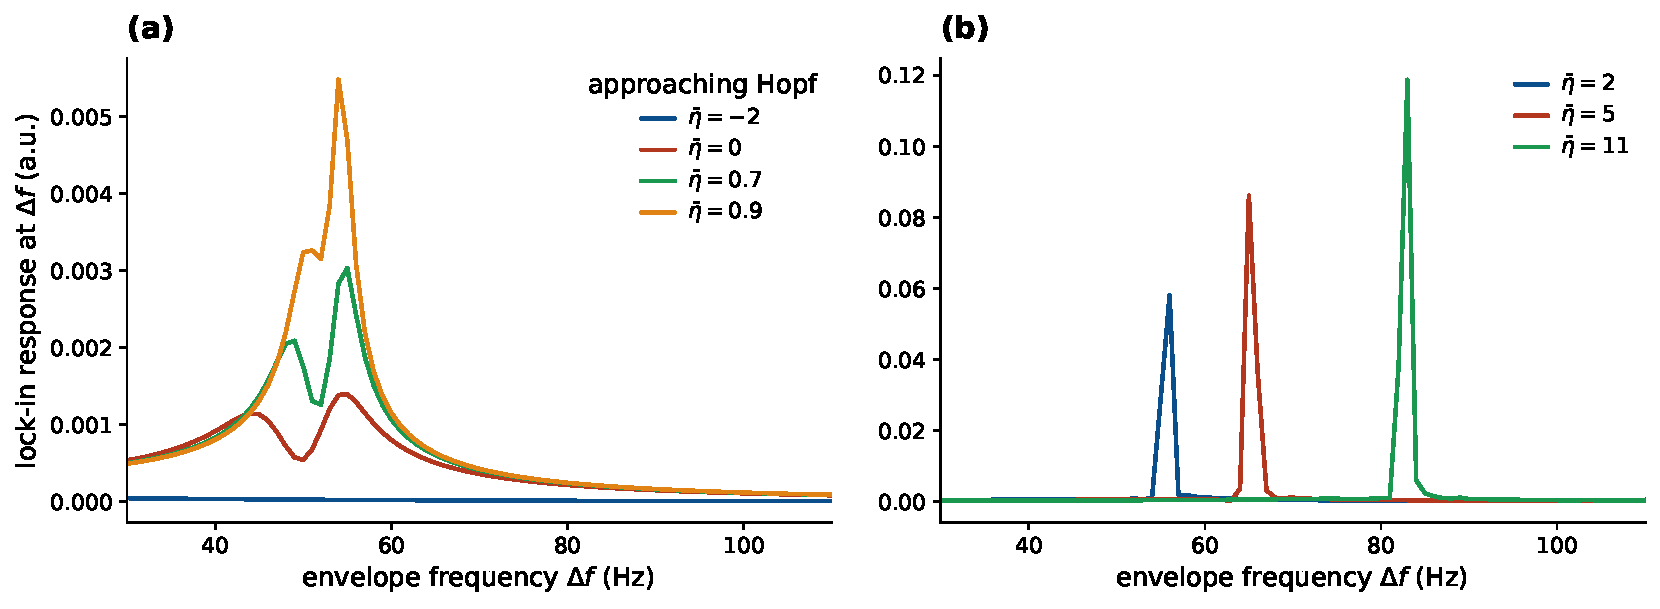
\includegraphics[width=\textwidth]{fig_nmm2_resonance_twotone.pdf}
\caption{\textbf{NMM2 PING gamma resonance (exact mean field, genuine two tones).}
Lock-in response of the excitatory rate $r_E$ at the envelope frequency $\Delta f$ under a
two-tone TI field (carrier $300$~Hz). \emph{(a)} (stable focus,
$\bar\eta<\bar\eta_{\rm Hopf}\!\approx\!1$) forced resonance at the gamma frequency
($f_0\!\approx\!55$~Hz), the peak growing $0.0014\!\to\!0.0030\!\to\!0.0055$ as the Hopf
is approached ($1/\gamma$ gain). \emph{(b)} (limit cycle,
$\bar\eta>\bar\eta_{\rm Hopf}$) entrainment of the autonomous gamma, the peak shifting
upward with $\bar\eta$ ($56\!\to\!65\!\to\!83$~Hz). The input carries no power at
$\Delta f$; the response is synthesized by the exact quadratic $v^2$ nonlinearity, with no
sigmoid anywhere in the model. Matched AM and two-tone drives agree at $\Omega$ to
$0.07\%$ well below the Hopf and to $4\%$ at $\bar\eta=0.9$, consistent with the JR
surrogate control (Fig.~\ref{fig:opp}d).}
\label{fig:nmm2_res}
\end{figure}

\subsection{What the mesoscale adds: coupling sets the gain at fixed detection}\label{sec:jcurve}
The resonance sweeps above drove the column toward the Hopf with the external input
$p$, but $p$ also shifts the operating point, entangling detection ($\Sig''$) with
amplification. The sharper, mechanistic statement is that the \emph{network coupling}
sets the gain on its own. In the JR column we vary the global connectivity $C$---the
coupling strength $J$---and, for each $C$, solve analytically for the drive $p(C)$ that
\emph{pins} the operating point $v^*$, so the detection gain $\Sig''(v^*)$ and the
open-loop detector amplitude $A_{\rm open}=\half\Sig''(v^*)\varepsilon^2 m$ are held
exactly constant. As $C\!\to\!C^*$ (the Hopf, $C^*\!\approx\!137$) the damping
$\gamma\!\to\!0$, the demodulated response grows $\sim$$27\times$ and the envelope
resonance sharpens (Fig.~\ref{fig:jcurve}a,b)---entirely a network effect, since
detection is frozen and only $\gamma$ changes. The recovered gain
$A_\Omega/A_{\rm open}$ tracks $1/\gamma$ before saturating near criticality
(Fig.~\ref{fig:jcurve}c); driving the same column to the Hopf through the input $p$
rather than the coupling $C$ yields the same gain--$\gamma$ relation, so the
amplification depends only on the distance to criticality, not on which parameter
delivers it. All these sweeps stay on the stable-focus side ($\gamma>0$), approaching
the supercritical Hopf from below: the $1/\gamma$ growth is the forced-resonance
susceptibility of a damped network, not entrainment of an autonomous cycle. On the
other side of the bifurcation the column oscillates on its own, and the demodulated
drive instead phase-locks that limit cycle within an Arnold tongue
(Fig.~\ref{fig:entrain}; also the entrainment side of Fig.~\ref{fig:res} and the LaNMM
and NMM2 maps)---$1{:}1$ frequency capture over a band that widens with drive,
quantified by the locking range rather than a diverging $1/\gamma$ gain, the two
coinciding only at onset. Because the drive is weak, on the autonomous side it biases
phase (timing) more than amplitude, consistent with the timing-not-rate signature
(\S\ref{sec:timing}).

\begin{figure}[t!]
\centering
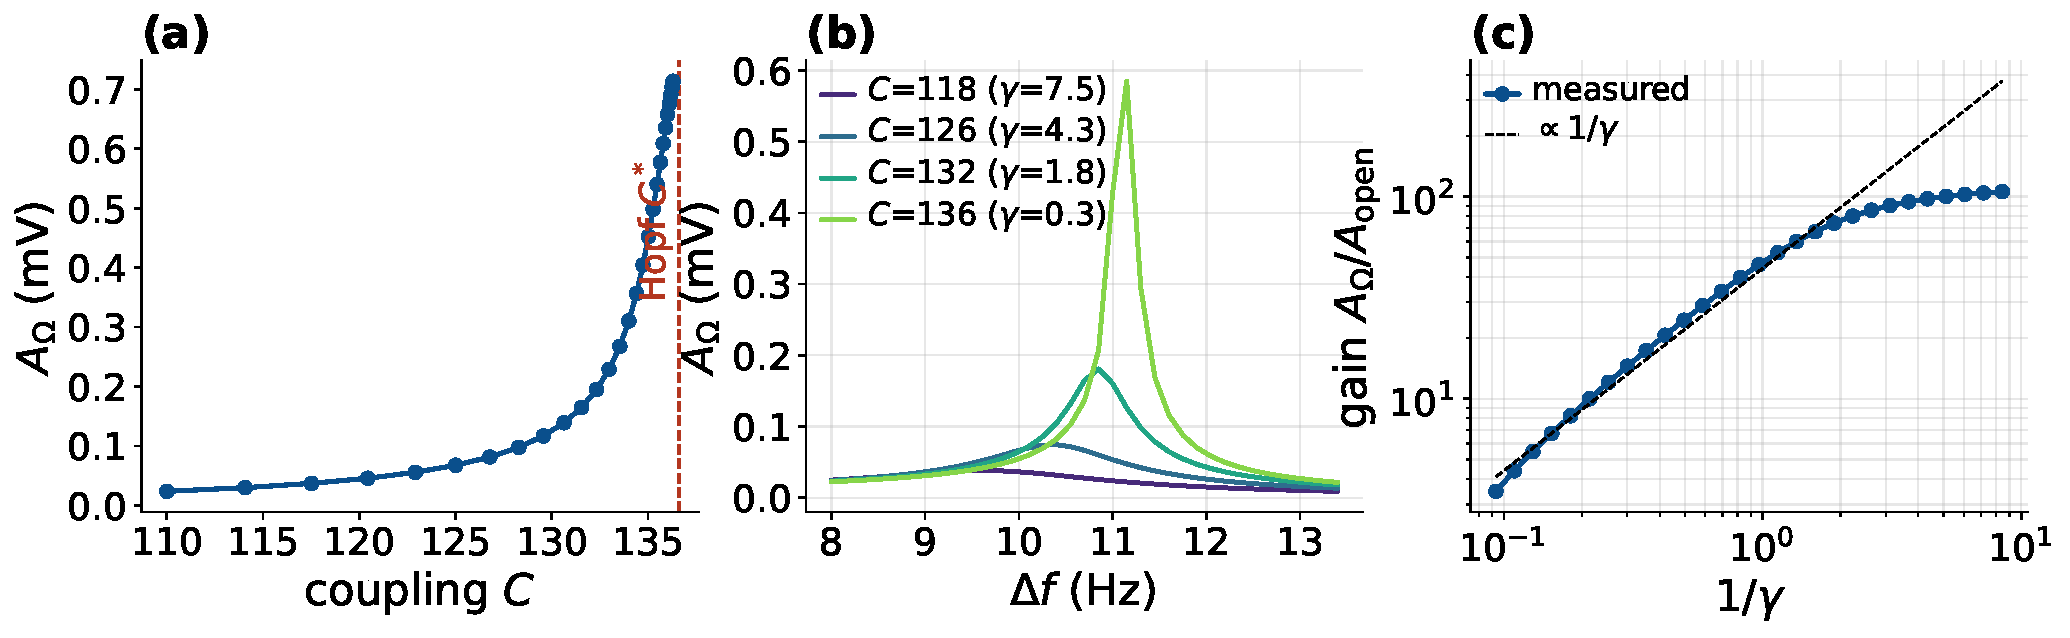
\includegraphics[width=\textwidth]{fig_jcurve.pdf}
\caption{\textbf{Coupling controls the amplification at fixed detection (Jansen--Rit).}
The operating point $v^*$ is pinned by co-solving $p(C)$, so $\Sig''(v^*)=-0.151$ and
$A_{\rm open}$ are held constant throughout. \emph{(a)} The demodulated $A_\Omega$ grows as the
coupling $C\,(=J)$ approaches the Hopf $C^*$ from the stable-focus side ($\gamma>0$). \emph{(b)} The envelope resonance
sharpens and grows as $C\!\to\!C^*$. \emph{(c)} The network gain
$A_\Omega/A_{\rm open}$ follows $1/\gamma$ (dashed) and saturates near the
bifurcation.}
\label{fig:jcurve}
\end{figure}

This becomes exact in the next-generation theory. In the NMM2 PING the coupling $C$ is
the \emph{literal} mean inter-neuron (QIF) synaptic weight $J$, and the demodulating
nonlinearity is the exact $v_E^2$ term, whose quadratic coefficient is a fixed
constant---so detection needs no pinning. Sweeping $J$ at fixed background drive
$\bar\eta$ toward the gamma Hopf $J^*$, the demodulated peak of $r_E$ grows as
$1/\gamma$ and saturates at criticality (Fig.~\ref{fig:nmm2_jcurve}): the heuristic JR
result, reproduced with the coupling \emph{and} the rectifier both derived rather than
assumed, and a direct counterpart of the coupling-controlled weak-field sensitivity of
QIF networks \cite{clusella2023}. The two columns realize one band-agnostic law in
their two native bands---alpha (JR) and gamma (NMM2): the single-cell nonlinearity
detects the envelope (coarse-grained into $\Sig''$, or the exact $v^2$), while the
sharp, tunable gain is the network's---a resonant amplification set by proximity to the
Hopf and adjustable through the coupling.

\subsection{The resonance amplifies envelope timing, not the mean rate}\label{sec:timing}
The demodulator feeds the network a baseband term and a line at the beat $\Omega$
(Eq.~\eqref{eq:taylor}), and the transfer $G(\Omega)$ of Eq.~\eqref{eq:gain} treats them
differently: $G(\omega_0)\propto1/(2\gamma\omega_0)$ diverges as the Hopf is approached,
while $G(0)\propto1/\omega_0^2$ stays flat. Pinning $v^*$ to hold detection fixed, as in
Fig.~\ref{fig:jcurve}, and driving the column toward the Hopf through the coupling, the AC
lock-in at the resonant beat $\Delta f=f_0$ grows $\sim$$17\times$, tracking $1/\gamma$
before saturating near criticality, while the DC shift of the mean pyramidal firing rate
stays within a few mHz of zero (Fig.~\ref{fig:timing}). The network amplifies the
envelope-locked AC response and not the DC rate, so a flat mean rate is the expected
signature even where TI is acting---the mesoscopic counterpart of the observation that TI
alters spike timing but not firing rate in the primate brain \cite{vieira2024}.

\subsection{Microscale confirmation: TI realigns spike timing in the QIF network}\label{sec:qif}
The mesoscale prediction has a direct microscale test, since NMM2 is the \emph{exact} mean
field of an all-to-all network of quadratic integrate-and-fire (QIF) neurons with
Lorentzian-distributed excitabilities
\cite{montbrio2015,ruffini2025rosetta,clusella2023}. Integrating that spiking network
($N=8000$ neurons per population, parameters identical to the PING mean field; Methods)
shows TI bunching spike \emph{times} into the beat cycle with only a small change in the mean
rate, on both sides of the gamma Hopf (Fig.~\ref{fig:qif_raster}). Below the Hopf (forced)
the field-free network fires asynchronously at a flat rate; with TI on, spikes condense
into envelope-locked bands (Fig.~\ref{fig:qif_raster}a,b). Above the Hopf (oscillatory) the
free-running gamma is \emph{gated} by the TI beat---forced cross-frequency modulation
(PAC), not frequency entrainment, since the $\approx$11~Hz detuning lies outside the
$1{:}1$ tongue: its bursts group into the $\Delta f=42$~Hz envelope while the intrinsic
$\sim$53~Hz gamma persists (Fig.~\ref{fig:qif_raster}c,d). Because the two rhythms coexist
in a nonlinear medium, the sigmoid mixes them into intermodulation sidebands in the
population rate---most prominently the direct $\Delta f$ line and the sum component near
$95$~Hz ($53\!+\!42$), with the difference tone near $11$~Hz (the detuning itself); this is
the spiking-network fingerprint of the same nonlinear frequency mixing that operates at the
macroscale, and it is the sideband signature of \emph{gating} rather than the frequency
pulling of entrainment. The spiking network reproduces
the exact NMM2 mean field (matched gamma spectrum and mean rate,
Fig.~\ref{fig:qif_timing}a), and across both regimes the mean rate rises only slightly
($\times1.07$--$1.11$) while the $\Delta f$ modulation depth of the population rate rises
from $0.01$--$0.03$ to $0.17$--$0.79$ (Fig.~\ref{fig:qif_timing}c). The same separation
appears per neuron rather than only in the population average: the spike vector strength at
$\Delta f$ rises from $0.044$ field-free to $0.334$ (forced) and $0.159$ (gated). Thus
envelope-locked timing modulation dominates rate modulation by roughly an order of magnitude---the spiking-level
counterpart of \S\ref{sec:timing} and a direct microscale analog of the in-vivo finding
that TI alters spike timing far more than firing rate \cite{vieira2024}.

\begin{figure}[t!]
\centering
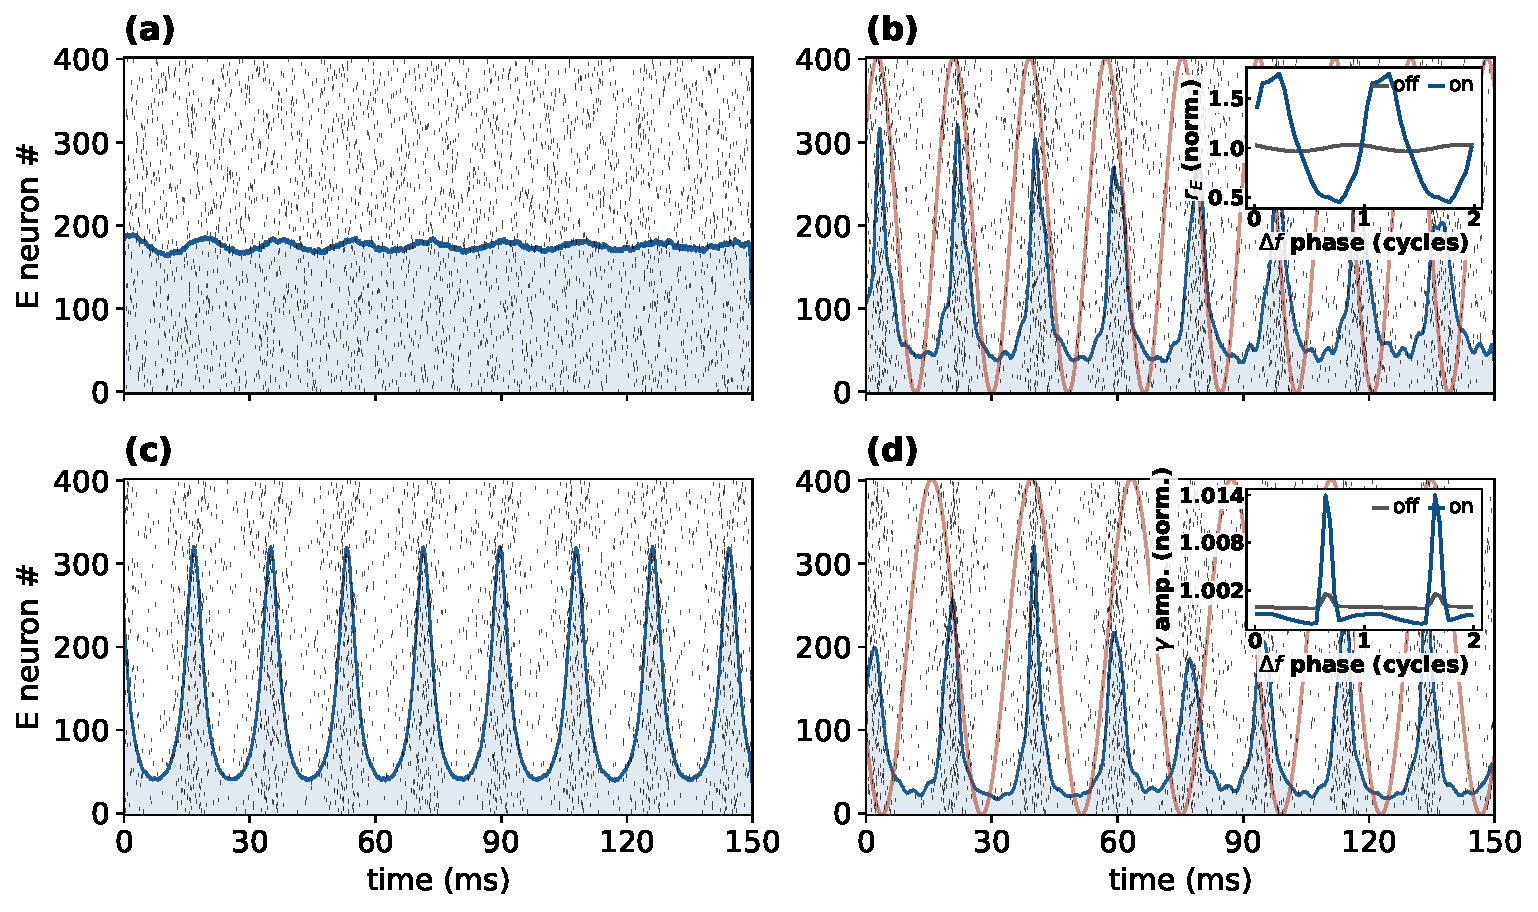
\includegraphics[width=\textwidth]{fig_qif_raster_twotone.pdf}
\caption{\textbf{QIF spiking network: TI realigns spike timing, not mean rate.} $N=8000$
excitatory and inhibitory quadratic integrate-and-fire neurons whose exact mean field is the
NMM2 PING circuit (Eq.~\eqref{eq:nmm2-ping}). The circuit's intrinsic rhythm is gamma
($\sim$53~Hz), so the beat is set in the gamma range (carrier $f_c=300$~Hz, genuine two
tones). Black ticks are $E$ spikes (400 of 8000), blue the population rate, red the TI
envelope; the bifurcation parameter is the common drive $\bar\eta$ (gamma Hopf at
$\approx$$1.1$). \emph{(a,b)} Forced ($\bar\eta=0.85$), TI off then on at
$\Delta f=55$~Hz: asynchronous firing becomes envelope-locked bunching.
\emph{(c,d)} Oscillatory ($\bar\eta=1.5$), TI off then on with the beat detuned to
$42$~Hz: the free-running gamma persists but gains a $\Delta f$-locked component. Because
the $\approx$11~Hz detuning places the beat outside the $1{:}1$ tongue, this is forced
cross-frequency \emph{gating}, not frequency capture (contrast
Fig.~\ref{fig:entrain}); the detuning is what certifies the locked component as a driven
effect. \emph{Insets}, each normalized to its own mean, folded on beat phase (off gray, on
blue): \emph{(b)} the population rate; \emph{(d)} the gamma-band \emph{amplitude}, since
taking the amplitude removes the gamma carrier so the near-commensurate $53/42$~Hz rhythms
cannot contaminate the fold. Both are flat with TI off.}
\label{fig:qif_raster}
\end{figure}

\subsection{Falsifiable predictions and tests}\label{sec:predictions}
The mechanism makes four sharp predictions, each with a clean experimental handle.
\begin{enumerate}[leftmargin=*]
\item \textbf{Carrier independence at fixed polarization.} Once the post-coupling
polarization $\varepsilon=\kappa(f_c)E_0$ is matched, the envelope response no longer
depends on $f_c$, even though the \emph{applied}-field threshold rises with $f_c$
through the membrane roll-off (Eq.~\eqref{eq:khz})---as single-neuron accounts also
predict \cite{opancar2025,mirzakhalili2020}. \emph{Test:} hold the in-zone
polarization fixed (raising $E_0$ to compensate the measured $\kappa(f_c)$) while
sweeping $f_c$; the network signature is a flat envelope response.
\item \textbf{Operating-point (PEIX) control and sign flip.} Because
$A_\Omega\propto\Sig''(v^*)$, the response scales with the curvature at the operating
point and \emph{reverses sign} across the inflection, vanishing at $v_0$ where the
gain $\Sig'$ (PEIX, Eq.~\eqref{eq:peix}) peaks. \emph{Test:} shift $v^*$ with tonic
drive, neuromodulation, or task state and read out the predicted scaling and sign
reversal of the TI response.
\item \textbf{Transduction class.} A weak smooth nonlinearity transduces $A^2$ and an
envelope follower transduces $A$ (\S\ref{sec:transduction}), and the two are separable at a
single matched target. The former gives $Y_\Omega\propto\varepsilon^2$ with a second-harmonic
ratio vanishing as $\varepsilon\!\to\!0$; the latter gives $Y_\Omega\propto\varepsilon$ with
the ratio pinned at $1/5$. \emph{Test:} sweep field amplitude off resonance (so that both
lines sit on the flat part of $G$) and read the log--log slope together with
$Y_{2\Omega}/Y_\Omega$; on resonance the network suppresses the second harmonic by
$\sim$$3\mathcal{Q}$ and the test must be corrected by an independently measured
$G(2\Omega)/G(\Omega)$.

\item \textbf{Frequency selectivity and state-dependence.} The response is largest
when $\Delta f$ matches a region's resonant rhythm and is amplified as $1/\gamma$ near
a bifurcation, so manipulations that move the operating point or the distance to the
Hopf---psychedelics, PV-interneuron dysfunction, attention, arousal---should scale,
and can abolish or sign-reverse, TI efficacy \cite{ruffini2025cfc}. \emph{Test:}
sweep $\Delta f$ through a region's intrinsic band across brain states and track the
resonant peak and its width.
\end{enumerate}

Table~\ref{tab:predictions} confronts these predictions---together with two corollaries
the mechanism already shares with published observations---against existing evidence.
Two are, in qualitative form, \emph{already supported}: TI alters spike timing but not
firing rate in vivo \cite{vieira2024} (our $G(\omega_0)\!\gg\!G(0)$ asymmetry,
\S\ref{sec:timing}--\ref{sec:qif}), and most pyramidal TI responses vanish when synaptic
transmission is blocked \cite{caldas2024} (a network, not single-cell, read-out). A
quantitative reanalysis of these datasets against the model is a natural next step.

\begin{table}[h]
\centering\small
\renewcommand{\arraystretch}{1.25}
\begin{tabular}{@{}p{0.27\textwidth} p{0.35\textwidth} p{0.30\textwidth}@{}}
\toprule
\textbf{Prediction (model basis)} & \textbf{Existing evidence} & \textbf{Sharp test} \\
\midrule
Transduction class: $Y_\Omega\propto\varepsilon^2$ and vanishing $Y_{2\Omega}/Y_\Omega$
(square law) vs.\ $\propto\varepsilon$ and $1/5$ (envelope following) & --- (a sharp new
prediction; untested) & Amplitude sweep off resonance; transfer-corrected harmonic ratio \\
Timing, not rate: TI amplifies the envelope-locked AC, not the DC mean rate
($G(\omega_0)\!\gg\!G(0)$) & \emph{Supported in vivo}: TI alters spike timing but not
firing rate, primate \cite{vieira2024} & Lock-in of spike timing at $\Delta f$ vs.\ the
mean-rate change \\
Network, not single-cell, read-out (population sigmoid + synaptic recurrence) &
\emph{Supported in vitro}: most pyramidal TI responses vanish under synaptic block
\cite{caldas2024} & Synaptic block should abolish the demodulated response \\
Carrier independence at fixed polarization (no $\omega_c$ in $A_\Omega$) & TI thresholds
inherit the carrier's $f_c$-dependence \cite{opancar2025,peripheral2023}; bare kHz weakly
effective \cite{esmaeilpour2020} & Fix in-zone polarization, sweep $f_c\!\to$ flat envelope
response \\
Operating-point ($\Sig''$) control and sign reversal across $v_0$ & Cell-type-specific TI
responses (PV vs.\ pyramidal) \cite{caldas2024} & Shift $v^*$ (neuromodulation/state)
$\to$ scaling and sign flip \\
Frequency selectivity, sharpened $\sim1/\gamma$ near criticality & --- (a sharp new
prediction; largely untested) & Sweep $\Delta f$ through a region's band across brain
states \\
\bottomrule
\end{tabular}
\caption{The mechanism's predictions confronted with existing in-vivo / in-vitro evidence.
Entries cite documented qualitative findings; quantitative reanalysis is left to future
work.}\label{tab:predictions}
\end{table}

\section{Discussion}\label{sec:discussion}
We have given a mesoscopic account of TI in which the firing-rate nonlinearity is a
square-law detector and proximity to a Hopf bifurcation turns the recovered beat component
into a sharp, frequency-selective response. This complements rather than competes with the
single-neuron ion-channel account \cite{mirzakhalili2020}: both are rectify-then-filter
demodulation, but ours is agnostic about which fast cellular nonlinearity supplies the
effective curvature, and it inherits the brain's own resonances, so a region's tuning is
set by its intrinsic dynamics just as a radio is tuned by its tank. Detection is a
population read-out of a coarse-grained single-cell nonlinearity; the amplification is the
emergent network property. Beyond contributing to the transfer's shape, the single cell
need only supply a fast nonlinearity that samples the carrier.

\textbf{Where the carrier-sampling nonlinearity may live.} The literature points to three
non-exclusive loci. (i)~\emph{Axonal Na$^+$ channels} at nodes and the AIS, where fast
voltage-gated Na$^+$ rectifies because activation outpaces inactivation
\cite{mirzakhalili2020,wang2023} and inactivation-mediated block passes the slow envelope
while removing the carrier \cite{opancar2025}. (ii)~\emph{Presynaptic terminals}, which
polarize $\sim$2--10$\times$ more than somata \cite{rahman2013,aberra2023,chakraborty2018}
and convert depolarization into release through a steeply nonlinear Ca$^{2+}$ relation.
Sensitivity is not speed, however: for an isopotential compartment $\tau_m=R_mC_m$ with
both quantities per unit area, so the time constant does not shrink with size---a small
bouton has small capacitance and correspondingly large input resistance. A terminal
therefore tracks a kHz carrier no better than a soma, and the short axonal time constants
come from high-conductance nodal membrane rather than from small size. Terminals are the
\emph{sensitive} locus, not the fast one, and the carrier sampling is supplied
by~(i). (iii)~\emph{Threshold spiking}, where a weak bias near threshold is rectified
through stochastic resonance \cite{liu2018,reato2010}. The same logic applies to TMS, whose
pulses carry kHz content that a $16$~ms soma attenuates by $\sim$50~dB, so it too must act
through fast elements whose chronaxie sets a corner near $\sim$800~Hz
\cite{barker1991,peterchev2013}.

\textbf{The conventional TI dose map is an assumption about physiology, not a consequence
of field physics.} The envelope is a mathematical property of a high-frequency waveform. It
is not itself a low-frequency field, and nothing in Maxwell's equations delivers it to a
neuron; biology must construct it. Targeting work since \cite{grossman2017} takes the
envelope-modulation amplitude $\mathcal{M}[A]=2\min(\varepsilon_1,\varepsilon_2)$ as the
spatial dose, which assumes $R(\mathbf{x})=\Phi(\mathcal{M}[A])$ for monotonic $\Phi$---that
the response depends on the envelope excursion \emph{alone}, and not separately on the
carrier baseline, the operating point or the orientation. That assumption is substantive,
and a weak smooth nonlinearity cannot satisfy it: the carrier average
Eq.~\eqref{eq:cycavg} is invariant under $A\to-A$, so its expansion contains only even
powers and no term proportional to $A$ exists. Square-law transduction is therefore the
generic perturbative answer and envelope following is the special case needing
justification, since recovering $A$ requires rectification (\S\ref{sec:transduction}) and
any \emph{smoothed} threshold reverts to $A^2$ as the field weakens.

We doubt there is a single universal TI mechanism. Near threshold a sharp channel or spike
nonlinearity may act as a rectifier and approximate envelope following; well below it, the
leading response of any smooth cellular nonlinearity is square-law mixing, filtered and
amplified by the network as described here. The empirical picture fits that split rather
than a clean envelope detector: primate recordings report incomplete demodulation, a timing
rather than rate effect, and a much weaker response to TI than to tACS \cite{vieira2024},
and peripheral-nerve work argues that some TI responses reflect carrier integration rather
than envelope extraction \cite{peripheral2023}. What settles it is not whether TI works but
which quantity it transduces, and \S\ref{sec:transduction} gives the measurement.

\textbf{The amplifier is not specific to TI.} A tACS field oscillates in the envelope band
directly and needs no demodulation, but it drives the same near-Hopf resonator. Sweeping
the coupling toward the alpha Hopf at \emph{pinned} operating point, a direct $\Delta f$
drive reproduces the same $1/\gamma$ growth and resonance sharpening as the demodulated TI
drive, linear in the field rather than square-law (Fig.~\ref{fig:tacs}). Prior work has
shown that recurrent coupling shapes tACS entrainment and sets the position of a network
resonance \cite{ali2013,ledoux2011}; what the pinned sweep adds is the isolation of the
gain itself, with detection held fixed so that only $\gamma$ varies. TI then differs from
tACS only by a demodulating front end that converts a kHz carrier's envelope into an
effective in-band drive; downstream, both share the criticality- and coupling-controlled
amplifier, so---matched for effective in-band drive---they should entrain alike.

\textbf{Amplification is critical slowing, of a mean-field kind.} Gain $\propto1/\gamma$ as
the damping vanishes at the Hopf is the dynamical signature of \emph{critical slowing}: a
susceptibility that diverges as a system approaches a bifurcation. Whether that warrants
the word ``criticality'' depends on the model. In the heuristic Jansen--Rit and LaNMM
columns the Hopf is a bifurcation of a finite-dimensional, fitted ODE, a near-bifurcation
statement rather than a phase transition. In the exact next-generation mean field it is
sharper: the reduction from the spiking QIF population is exact in the thermodynamic limit
and $(r,v)$ are genuine \emph{order parameters}, conformally related to the
Kuramoto--Daido order parameter through the Ott--Antonsen ansatz
\cite{ott2008,montbrio2015}, so the Hopf is a true macroscopic transition and the
$1/\gamma$ gain its diverging susceptibility. One qualifier keeps this honest. Because the
reduction assumes all-to-all coupling the critical point is \emph{mean-field}: it delivers
temporal critical slowing but no diverging \emph{spatial} correlation length, so the column
realizes the temporal-susceptibility face of criticality and not the scale-free spatial
one. With $J$ as the control parameter (Fig.~\ref{fig:nmm2_jcurve}), TI drives a population
toward a genuine, if mean-field, critical point and reads out its susceptibility.

\textbf{Prior work already places the operative nonlinearity in the network.} Recurrent
excitatory coupling accounts for tACS entrainment and yields an Arnold tongue
\cite{ali2013}; the dynamical transfer function of an E--I network shows a resonance whose
position depends on recurrent coupling \cite{ledoux2011}; an amplitude-modulated
high-frequency drive phase-locks a cortical model to its envelope through the same target
engagement as low-frequency tACS \cite{negahbani2018}; and comparing neuron models directly,
integrate-and-fire membranes fail to reproduce observed TI behavior while
Hodgkin--Huxley ones succeed \cite{plovie2025}. The general case for stimulation as
interaction with ongoing dynamics has been made explicitly \cite{krause2023}. What we add
is the pair of factors---$\Sig''$ as the detector in closed form, $1/\gamma$ as the
amplification tied to a measurable relaxation time---and, downstream of both, that the
transduced quantity is $A^2$ rather than $A$, which this work does not distinguish.

\textbf{The amplitude budget does not close at human field strengths.} Two hurdles stand
between a transcranial field and a response at $\Delta f$, and they need different answers.
The first is that weak fields barely move a membrane: measured coupling is
$0.12$--$0.21$~mV per V/m in hippocampus \cite{bikson2004,deans2007} and up to
$\sim$$0.5$~mV per V/m for cortical L5/6 pyramidal cells \cite{radman2009}, human cortex
sees about $0.8$~V/m at 2~mA \cite{huang2017,huang2017corr}, and most applied current is
shunted through scalp and skull \cite{voroslakos2018}. The field shifts a soma by a few
tenths of a millivolt against the $\sim$$23$~mV separating rest from threshold
\cite{koga2010}. This is as true of tACS as of TI. The second hurdle belongs to TI alone:
its field carries no power at $\Delta f$, so the response there must be manufactured, and
that is what $\Sig''$ does. The two answers do not substitute for each other. Resonance
clears the first---a population near its own bifurcation responds to a weak push far more
strongly than an isolated cell---but not the second, because it amplifies TI and tACS alike
and cancels when the two are compared.

The resonance buys a factor of order ten. With $\tau=1/\gamma$ the reverberation time, the
gain at resonance relative to the same circuit's response to a steady input is
$\mathcal{Q}=\pi f_0\tau$. Cortical population activity relaxes over a few hundred
milliseconds \cite{wilting2018}, giving $\mathcal{Q}$ of order $10$ at $f_0=10$~Hz---an
order of magnitude, not a value, since that timescale is wideband rather than
alpha-specific. Gain also costs bandwidth: the resonance is $1/(\pi\tau)$ wide, about
$1$~Hz, so a $\Delta f$ fixed at a group-mean alpha will drift outside it during a session.
At equal field strength TI is far weaker than tACS. With per-carrier polarizations
$\varepsilon_{1,2}$ the demodulated drive is
$\half\Sig''\varepsilon_1\varepsilon_2$ against $2\Sig'\varepsilon$ for tACS at the same
peak polarization, a ratio $\eta=\Sig''\varepsilon/4\Sig'$ proportional to
$\varepsilon$: a square-law detector gets \emph{less} efficient as the signal weakens.
Formally $\eta$ reaches unity near $\varepsilon\approx7$~mV, but that is the order of the
distance to threshold and lies outside the expansion's validity, so parity is not reachable
by this route rather than merely expensive. At $1$~V/m with a $1$~kHz carrier TI comes out
$\sim$$300\times$ weaker than tACS if the carrier reaches a fast nodal compartment, and
$\sim$$10^6\times$ weaker if it reaches only the soma. What TI buys for that price is
targeting: a field applied directly at $\Delta f$ cannot be steered to a deep structure,
whereas two kHz beams can.

The same nonlinearity explains why TI works in rodents and disappoints in humans. A mouse
brain sees $\sim$$383$~V/m from a TI montage while optimized human montages reach
$0.24$--$0.57$~V/m at depth \cite{rampersad2019}, a field ratio of order $10^3$. A
nonlinear detector amplifies that disparity, but not by the full square: at mouse field
strengths the polarization reaching the detector is $\varepsilon\!\sim\!18$~mV, roughly
$80\%$ of the way to threshold, so the transfer saturates and the small-signal expansion
fails. Evaluating the full sigmoid gives a drive ratio of order $10^4$ where extrapolating
the square law would predict $10^6$. The rodent experiment is therefore not the human
experiment scaled down: the mouse is driven into saturation while the human, at
$\varepsilon\!\sim\!0.02$~mV, sits deep in the perturbative regime where the quadratic
penalty is worst. A network model finding that TI needs $\sim$$100\times$ the tACS
amplitude \cite{karimi2024} is consistent with a nonlinear detector operating there. What
survives is the mechanism, not a solution to the dose problem---and it names the three
quantities worth improving: the carrier's access to a fast compartment, the operating point
through $\Sig''$, and proximity to the bifurcation through $\mathcal{Q}$.

\textbf{Limitations.} The field enters the population transfer directly; we treat the
field-to-nonlinearity coupling $\kappa(f_c)$ phenomenologically rather than modeling
channel kinetics, and $\varepsilon$ should be read as post-coupling polarization. The
population sigmoid is a coarse-grained stand-in for distributed single-cell nonlinearities.
JR alpha near this Hopf is high quality-factor, so the stable-side peaks are narrow and
would be broadened by noise and population heterogeneity; the columns here are single,
deterministic and noiseless, and coupled noisy columns with an explicit $\kappa(f_c)$
remain the natural next step. The human evidence is also not uniformly positive: a
controlled study found peripheral but no central effects \cite{iszak2023}, and a systematic
review reports that occipito-parietal TI did not modulate alpha power
\cite{mansourinezhad2025}. The narrowband prediction turns the second into a design
question---whether $\Delta f$ tracked individual alpha closely enough to stay inside a
$\sim$$1$~Hz response band---which is a prediction to be tested, not an explanation to be
assumed.

\section{Conclusion}
In the weak-field limit any smooth cellular nonlinearity transduces the \emph{square} of
the TI envelope rather than the envelope itself: the carrier average contains only even
powers, so the leading response is $\tfrac14 g''(v^*)A^2$ and there is no term linear in
$A$. Recovering $A$ would require rectification, and any smoothed threshold reverts to
$A^2$ as the field weakens. The population sigmoid is thus not an exotic detector but the
generic perturbative one, and the beat component it generates,
$\half\Sig''(v^*)\varepsilon_1\varepsilon_2$, is what a second-order-synapse network near
a Hopf then amplifies as $1/\gamma$. A fast single-cell nonlinearity---Na$^+$ at nodes or
the AIS, persistent Na$^+$, presynaptic terminals---need only deliver the carrier to that
transfer; the mechanism is agnostic about which one does.

Both halves are state-dependent, detection through $\Sig''(v^*)$ and amplification through
$\gamma$, so TI efficacy is as much a property of brain state as of the stimulus: largest
near a bifurcation, tunable by connectivity at fixed detection, and reversible in sign by
shifting the operating point. That the same amplifier serves a direct in-band drive means
tACS inherits it too, which is why resonance cannot recover TI's square-law penalty.

Because the transduced quantity is $A^2$ and not $A$, the mechanism predicts a spatial
response map that is the conventional envelope map reweighted by the dominant local
polarization, a response quadratic rather than linear in field amplitude, and an
envelope-locked spectrum without the harmonic ladder an envelope follower would produce.
These are measurable, and they are what would settle which quantity TI actually
transduces.

\section*{Code and data availability}
All simulation and figure-generation code, the committed datasets, and a one-command
reproduce script (\texttt{run\_all.py}) are openly available at
\url{https://github.com/giulioruffini/TI-demodulation-paper}, archived at
\href{https://doi.org/10.5281/zenodo.21009618}{Zenodo (doi:10.5281/zenodo.21009618)}.
The repository \texttt{README} documents the per-figure script mapping (a
figure$\rightarrow$script table) and the dependency order, so every figure in this note can
be regenerated from the committed inputs. The code is released under CC-BY-4.0.

\section*{Acknowledgments}
GR, BM, AJ and FC have received funding from the European Research Council (ERC) under the
European Union's Horizon 2020 research and innovation programme (grant agreement No 855109,
GALVANI).
% TODO before submission: funding for SC (IN, UMH-CSIC) and CM (IFISC, UIB-CSIC).
% IOP requires the funding agency AND grant number disclosed for all support.

\ifjne
\section*{Competing interests}
% ---------------------------------------------------------------------------
% DRAFT -- must be confirmed by all seven authors before submission. IOP treats
% this as mandatory and asks for financial and non-financial interests alike.
% The text below is inferred from affiliations and has been checked by nobody.
% ---------------------------------------------------------------------------
GR is Chief Scientific and Technology Officer of Neuroelectrics, which develops and
commercializes transcranial stimulation devices. BM, AJ and FC are affiliated with
Neuroelectrics. The remaining authors declare no competing interests.

\section*{Author contributions}
% CRediT roles. DRAFT -- each co-author must confirm their own line before
% submission; the assignment below is inferred from the project record.
Using the CRediT taxonomy: \textbf{G.~Ruffini} --- conceptualization, methodology,
formal analysis, software, writing (original draft), supervision, funding acquisition.
\textbf{B.~Mercadal} --- methodology, formal analysis, writing (review and editing).
\textbf{A.~Just} --- software, validation, visualization, writing (review and editing).
\textbf{R.~de Palma Aristides} --- software, validation, writing (review and editing).
\textbf{F.~Castaldo} --- methodology, writing (review and editing).
\textbf{S.~Canals} --- conceptualization, writing (review and editing).
\textbf{C.~Mirasso} --- conceptualization, methodology, writing (review and editing).
All authors read and approved the final manuscript.
\fi

\section*{Declaration of generative AI and AI-assisted technologies in the manuscript
preparation process}
% IOP asks for the tool name and version, and expects prior drafts and prompts
% to be retained. TODO: pin the versions actually used before submission.
During the preparation of this work the authors used Anthropic Claude and OpenAI ChatGPT to
streamline the narrative and to assist with code and figure generation from data the authors
produced. The authors reviewed and edited all resulting content and take full responsibility
for the content of the published article.

\bibliographystyle{unsrt}
\bibliography{references}

\fi
\ifappendices
\clearpage
\appendix
\renewcommand{\thefigure}{S\arabic{figure}}
\setcounter{figure}{0}
% Appendices are last; each starts on a fresh page (explicit \clearpage before
% every appendix \section) so no appendix heading is orphaned at a page foot.
\makeatletter
\let\ne@stdsection\section
\renewcommand{\section}{\clearpage\ne@stdsection}
\makeatother

\section{Notation and units}\label{app:notation}
These neural-mass models are phenomenological: potentials are in mV, firing rates in
s$^{-1}$ ($\equiv$Hz), time constants in ms, and frequencies in Hz, unless noted; a
``--'' marks a dimensionless quantity. A few glyphs are reused across the four models
(JR, LaNMM, NMM2/MPR, QIF) by long-standing convention; these are disambiguated by
context and flagged below. In particular, $A$ is the excitatory PSP \emph{gain} in the
JR/LaNMM synapses and nothing else; the applied-field modulation amplitude is
$\varepsilon$ in JR and LaNMM alike, and $A_f$ in NMM2/QIF. These are not
interchangeable units. In JR and LaNMM the field is a membrane polarization in mV
entering the sigmoid argument, so $\varepsilon$ is measured against the sigmoid voltage
scale $1/\rho\approx1.8$~mV, which is the same in both models. In NMM2/QIF the field
enters the excitatory membrane current in the dimensionless MPR units of $v_E$, and
$A_f$ carries no volt scale at all. Likewise $C$ is the JR connectivity constant and the
NMM2 global synaptic gain $C\,(\equiv J)$.

\renewcommand{\arraystretch}{1.18}
{\footnotesize
\begin{longtable}{@{}p{0.16\textwidth} p{0.62\textwidth} p{0.16\textwidth}@{}}
\toprule
\textbf{Symbol} & \textbf{Meaning} & \textbf{Units} \\
\midrule
\endfirsthead
\toprule
\textbf{Symbol} & \textbf{Meaning} & \textbf{Units} \\
\midrule
\endhead
\midrule \multicolumn{3}{@{}l}{\textit{Firing-rate nonlinearity (sigmoid)}} \\*
$\Sig(v)$ & population firing-rate transfer function & s$^{-1}$ \\
$\Sig'(v),\,\Sig''(v)$ & sigmoid slope and curvature; $\Sig''$ sets the demodulation gain & s$^{-1}$mV$^{-1,-2}$ \\
$e_0$ & half the maximal firing rate ($\Sig\!\to\!2e_0$ as $v\!\to\!\infty$) & s$^{-1}$ \\
$v_0$ & sigmoid inflection (half-maximal) potential & mV \\
$\rho$ & sigmoid slope parameter & mV$^{-1}$ \\
$v^{*}$ & operating point (field-free fixed point of $v$) & mV \\
$v=y_1-y_2$ & net pyramidal membrane potential (LFP proxy) & mV \\
PEIX & Population Excitation--Inhibition Index (a $\Sig'$-based brain-state index) & -- \\
\midrule \multicolumn{3}{@{}l}{\textit{Single-column Jansen--Rit}} \\*
$A,\,B$ & excitatory, inhibitory PSP gains & mV \\
$a,\,b$ & excitatory, inhibitory synaptic rates (inverse time constants) & s$^{-1}$ \\
$y_1,\,y_2$ & excitatory, inhibitory post-synaptic potentials & mV \\
$C,\,C_1\!-\!C_4$ & intracolumn connectivity constants & -- \\
$p$ & external input rate; JR bifurcation parameter & s$^{-1}$ \\
\midrule \multicolumn{3}{@{}l}{\textit{Applied TI field and coupling}} \\*
$s(t),\,e(t)$ & applied TI field perturbation, AM or two-tone (JR; LaNMM) & mV \\
$\varepsilon$ & field modulation amplitude, JR and LaNMM (a membrane polarization entering the sigmoid argument) & mV \\
$A_f$ & field modulation amplitude, NMM2/QIF (in the dimensionless MPR units of $v_E$) & -- \\
$m$ & modulation depth & -- \\
$f_c,\ \omega_c\!=\!2\pi f_c$ & carrier frequency & Hz, rad\,s$^{-1}$ \\
$f_1,f_2$ & the two applied carrier tones ($f_c\!=\!(f_1\!+\!f_2)/2$) & Hz \\
$\Delta f,\ \Omega\!=\!2\pi\Delta f$ & envelope (beat) frequency, $\Delta f\!=\!f_2\!-\!f_1$ & Hz, rad\,s$^{-1}$ \\
$E(t),\ \delta V(t)\!=\!\lambda E$ & applied field; induced membrane perturbation & V\,m$^{-1}$; mV \\
$\lambda$ & lumped (polarization-length) field-to-membrane coupling & mV\,/\,(V\,m$^{-1}$) \\
$\kappa(f_c)$ & applied-field-to-polarization coupling & mV\,/\,(V\,m$^{-1}$) \\
$H_m(\omega),\ \tau_m$ & somatic membrane low-pass and its time constant & --; ms \\
$\tau$ & fast-element (node/AIS/terminal) time constant & ms \\
\midrule \multicolumn{3}{@{}l}{\textit{Network dynamics, response, and bifurcation}} \\*
$\lambda_\pm=-\gamma\pm i\omega_0$ & leading Jacobian eigenvalue pair & s$^{-1}$ \\
$\gamma$ & damping of the critical mode ($\propto$ distance to the Hopf) & s$^{-1}$ \\
$\omega_0,\ f_0\!=\!\omega_0/2\pi$ & natural (Hopf) frequency & rad\,s$^{-1}$, Hz \\
$\mathcal{Q}=\omega_0/2\gamma=\pi f_0\tau$ & resonance quality factor ($\tau=1/\gamma$ the reverberation time) & -- \\
$G(\Omega)$ & network resonance gain (Lorentzian, $\propto\!1/\gamma$ at $\omega_0$) & -- \\
$A_\Omega$ & demodulated response: lock-in amplitude of $v$ at $\Omega$ & mV \\
$A_{\rm open}$ & same lock-in, open loop (detector only, no recurrence); $A_\Omega/A_{\rm open}$ dimensionless & mV \\
$I,\,Q$ & in-phase, quadrature lock-in components & mV \\
$C^{*},\,J^{*}$ & coupling at the Hopf (criticality) & -- \\
\midrule \multicolumn{3}{@{}l}{\textit{Laminar model (LaNMM)}} \\*
$P_1,\,P_2$ & deep (alpha) and superficial (gamma) pyramidal populations & -- \\
PV,\,SS,\,SST & parvalbumin, stellate, somatostatin interneurons & -- \\
$I_0$ & flat (DC) drive offset in $e(t)$ & mV \\
\midrule \multicolumn{3}{@{}l}{\textit{Exact mean field (NMM2 / MPR) and QIF network}} \\*
$r_E,\,r_I$ & population firing rates (E, I) & s$^{-1}$ \\
$v_E,\,v_I$ & mean membrane potentials (E, I), in dimensionless MPR units & -- \\
$\eta_j,\ \bar\eta$ & per-neuron excitability; mean excitability (= common drive, bifurcation param.) & -- \\
$\Delta$ & Lorentzian half-width of $\eta_j$ (excitability heterogeneity) & -- \\
$\tau_E,\tau_I,\tau_a,\tau_g$ & E, I membrane and AMPA, GABA synaptic time constants & ms \\
$C\,(\equiv J)$ & global synaptic coupling (inter-population gain) & -- \\
$A_{ee},A_{ei},A_{ie},A_{ii}$ & synaptic weight matrix $(1,1,1,2)$ & -- \\
$s_E,\,s_I$ & second-order synaptic activations; $\hat K_a,\hat K_g$ their operators & s$^{-1}$ \\
$V_j,\ V_{\rm peak}$ & QIF neuron potential; spike/reset threshold & mV \\
$N$ & neurons per population (QIF; $N=8000$) & -- \\
$A_\Omega/\langle r_E\rangle$ & $\Delta f$ modulation depth (envelope-locked timing metric) & -- \\
\bottomrule
\caption{Symbols, meanings, and (nominal) units. Reused glyphs are disambiguated by
context; see the head note on $A$ and $C$.}\label{tab:notation}
\end{longtable}}

\section{TI requires detection: the Stuart--Landau normal form amplifies but cannot demodulate}\label{app:sl}
Amplification and detection are separable, and the universal Hopf normal form makes the
separation sharp. The Stuart--Landau equation \cite{pikovsky2001} is
\begin{equation}
\dot z=(a+i\omega_0)z-|z|^2z+F(t),\qquad \gamma\equiv-a>0\ \ (\text{stable side}),
\label{eq:sl}
\end{equation}
driven by the TI field $F$. Expanding $z=\sum_k Z_k(t)e^{ik\omega_c t}$ in carrier
harmonics with slowly varying envelopes, the field forces only $k=\pm1$ and the cubic feeds
index $k=l-p+q$. The odd-$k$ subspace is therefore invariant and attracting: if every even
$Z_k$ vanishes, then for even $k$ both sources vanish---$F_k=0$, and $l-p+q$ cannot be even
with $l,p,q$ odd---leaving $\dot Z_k=[a+i(\omega_0-k\omega_c)]Z_k$, which decays at rate
$\gamma>0$. So $z$ lives only on odd carrier harmonics, to all orders in $\varepsilon$. The
beat line is a \emph{baseband} signal and would sit in $k=0$; since $Z_0\equiv0$, the
response at $\Delta f$ is identically zero. An \emph{even} nonlinearity instead produces a
nonzero $k=0$ term through $\cos^2\omega_c t\to\half$---the very line the odd cubic cannot
make. Numerically ($a=-0.5$, $f_0=10$, $f_c=100$~Hz, $\varepsilon=0.5$), a square-law
detector on the same field gives a $\Delta f$ lock-in of $2.5\times10^{-1}$ while
$\mathrm{Re}\,z$ gives $\sim$$2\times10^{-8}$, at the numerical floor. Driven instead
directly in band, the same equation shows the forced $1/\gamma$ growth toward the Hopf.

The normal form thus responds to tACS but is blind to TI. Amplification is the
model-independent near-Hopf susceptibility, shared with any normal-form resonator;
detection is the model-specific even-order term the normal form lacks. A critical
resonator alone cannot demodulate.

\section{Vocabulary and metrics}\label{sec:vocab}
``Entrainment'' is used in several senses, and our system can exhibit more than one, so
we fix the vocabulary. We reserve \emph{entrainment} for its dynamical-systems
meaning, frequency/phase locking of a \emph{self-sustained} oscillator to an external
rhythm confined to an Arnold tongue \cite{pikovsky2001}, and distinguish it from two
related read-outs.
\emph{(i) Forced response.} Below the Hopf the column does not oscillate on its own; the
field elicits a driven response whose susceptibility we quantify by the lock-in amplitude
of the read-out at the beat $\Delta f$ (Eq.~\eqref{eq:lockin}), and there is no autonomous
rhythm to entrain (J-curve, timing, tACS).
\emph{(ii) Frequency entrainment.} Above the Hopf the column free-runs at $f_0$; genuine
entrainment means its dominant frequency is \emph{pulled} to $\Delta f$. We test this with
the dominant output frequency $f_{\rm out}$ (largest non-DC FFT peak) and the $1{:}1$
criterion $|f_{\rm out}-\Delta f|<0.3$~Hz, mapping the Arnold tongue and locking range
(Fig.~\ref{fig:entrain}); we use $f_{\rm out}$ rather than a phase-locking value
\cite{lachaux1999} because, when an autonomous rhythm and a driven component coexist,
instantaneous-phase estimates conflate them whereas the dominant-frequency test isolates
true frequency capture.
\emph{(iii) Envelope locking / gating.} A periodic drive can instead modulate the
\emph{amplitude} of a persisting rhythm at the beat without capturing its
frequency---phase--amplitude coupling \cite{canolty2010,tort2010}. We quantify this by
the $\Delta f$-locked component of the population rate (lock-in of $r_E$ at $\Delta f$,
equivalently the rate \emph{folded} on the $\Delta f$ beat phase---averaged over many beat
cycles as a function of phase within a single cycle, so that everything not locked to
$\Delta f$ averages away), which isolates the driven envelope from the intrinsic rhythm. The distinction is load-bearing: the same word would
otherwise denote a frequency capture (ii) and an amplitude gating (iii) that are
dynamically different---so we label frequency capture \emph{entrainment} and amplitude
modulation of a persisting rhythm \emph{gating}, reporting the metric appropriate to each
(the above-Hopf QIF panel, with its $\sim$11~Hz detuning, is a case of gating, not
entrainment).

The Arnold-tongue protocol for Fig.~\ref{fig:entrain} places the column on the limit-cycle side (input $p$ between the SNIC and the Hopf, free-running at $f_0(p)$) and drives it with $s(t)=\varepsilon\cos\Omega t$; the implementation, including the grid widths and the clipping check, is in the released code. One subtlety is worth stating: as onset is approached the cycle amplitude vanishes and the tongue merges into the forced-resonance bandwidth, so the supercritical locking range and the subcritical $1/\gamma$ susceptibility coincide there by construction---which is why responsiveness peaks at criticality on both sides.

\section{Supplementary figures}

\begin{figure}[t!]
\centering
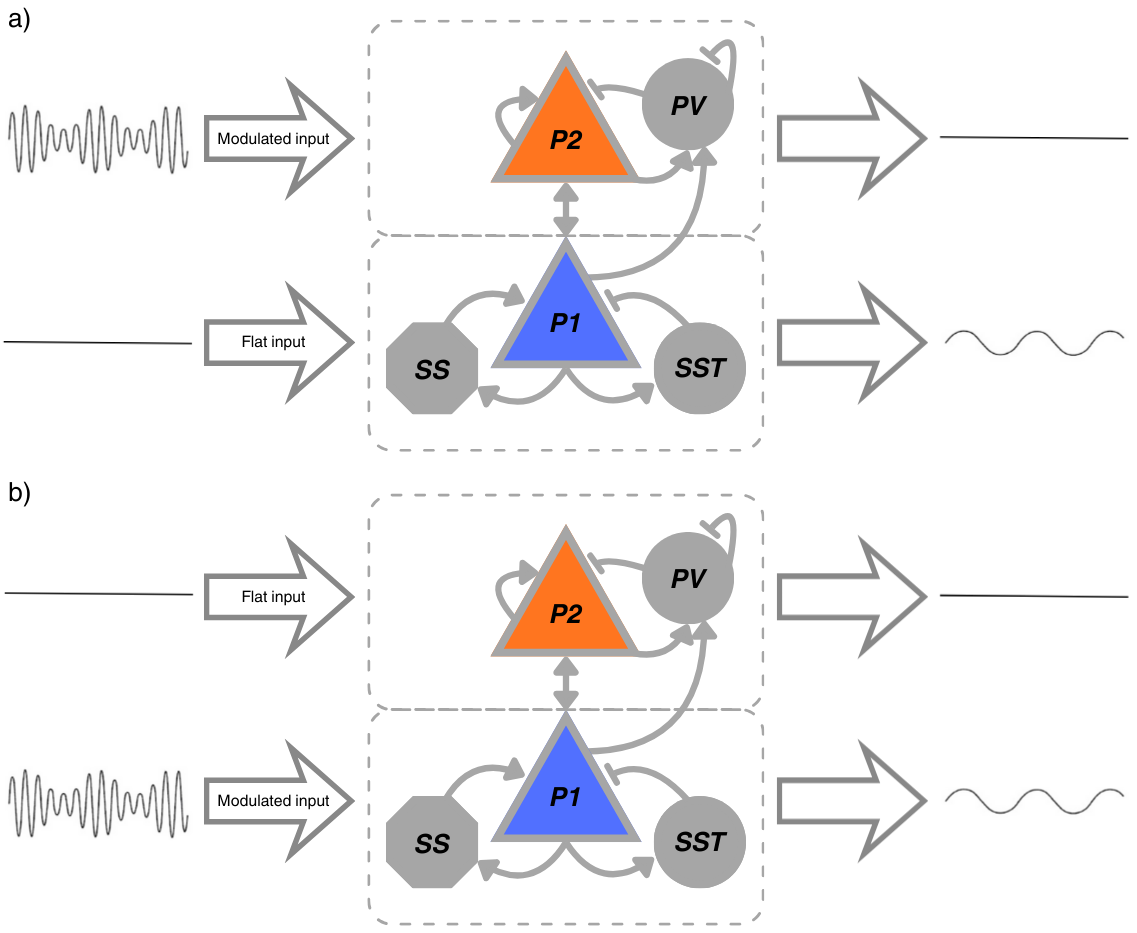
\includegraphics[width=0.85\textwidth]{fig_lanmm_setup.png}
\caption{\textbf{Stimulation setup in a LaNMM column.} The column couples a
superficial PING subcircuit (pyramidal $P_2$ + PV; gamma) and a deep JR
subcircuit (pyramidal $P_1$ + SS + SST; alpha). \emph{(a)} the TI field drives
$P_2$ while $P_1$ receives a flat drive; \emph{(b)} the TI field drives $P_1$
while $P_2$ is flat. Through the sigmoid nonlinearities and $P_1$--$P_2$ coupling,
the slow envelope is transferred to the column: $P_2$ carries the modulated fast
carrier, while $P_1$ exposes the recovered low-frequency beat component (right traces).}
\label{fig:lanmm_setup}
\end{figure}



\begin{figure}[t!]
\centering
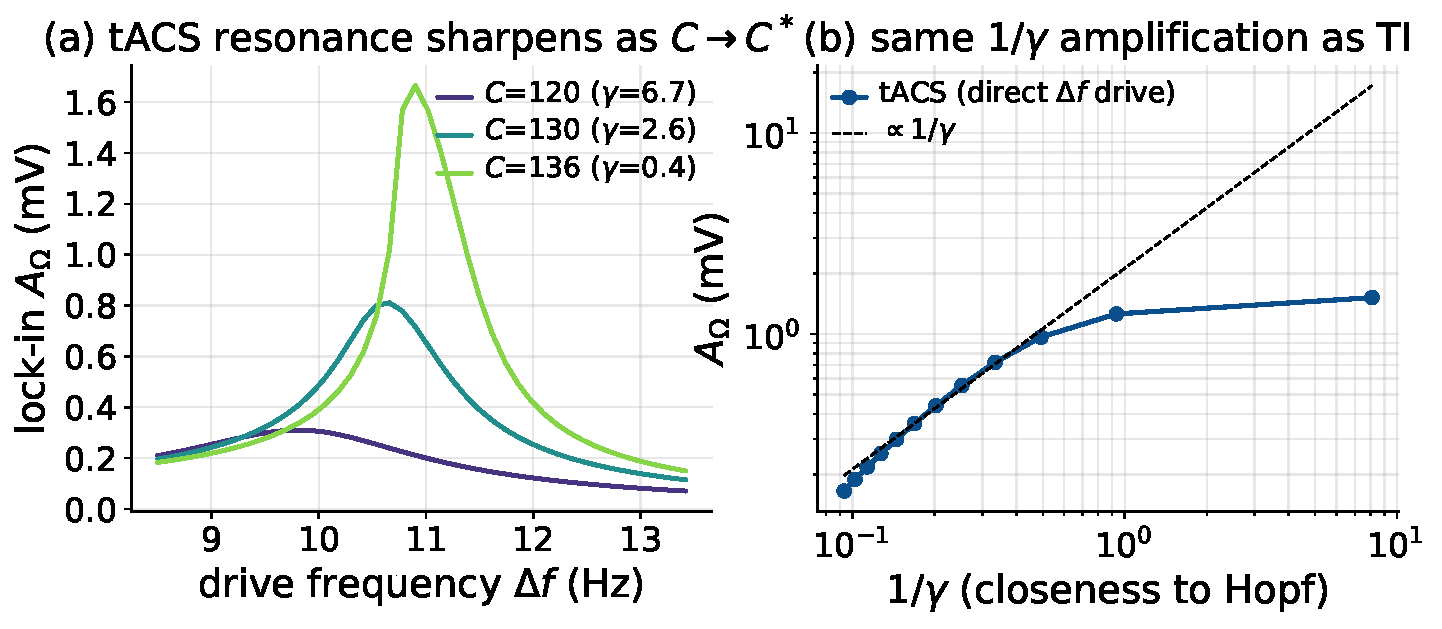
\includegraphics[width=0.92\textwidth]{fig_tacs_jcurve.pdf}
\caption{\textbf{tACS shares the network amplifier (Jansen--Rit).} A direct
low-frequency (tACS) drive at $\Delta f$ enters the column without a carrier, so it
needs no demodulation, but feeds the same near-Hopf resonator. With the operating point
pinned, sweeping the coupling $C\,(=J)$ toward the alpha Hopf: \emph{(a)} the lock-in
resonance at $\Delta f$ sharpens and grows as $C\!\to\!C^*$; \emph{(b)} the response
grows as $1/\gamma$ (dashed) and saturates near criticality---the same network
amplification as the demodulated TI drive (Fig.~\ref{fig:jcurve}), but linear in the
field rather than square-law. Throughout, the column is a stable focus ($\gamma>0$).}
\label{fig:tacs}
\end{figure}

\begin{figure}[t!]
\centering
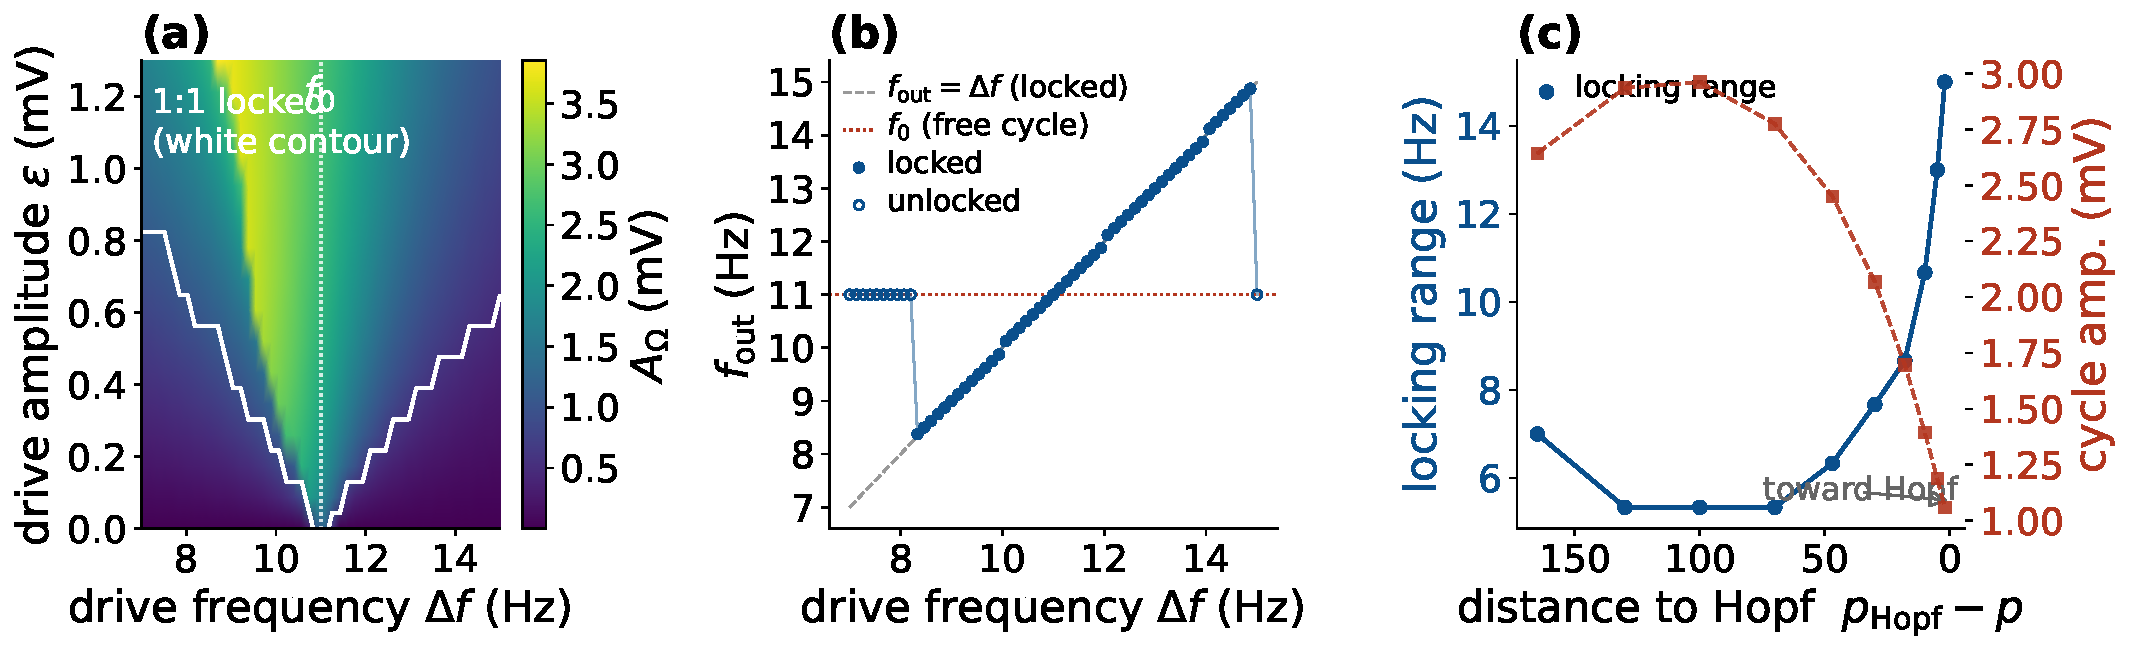
\includegraphics[width=\textwidth]{fig_entrainment.pdf}
\caption{\textbf{Above the Hopf: entrainment, not $1/\gamma$ amplification (Jansen--Rit).}
The column is set in its autonomous alpha limit cycle ($p=250$, $f_0\!\approx\!11$~Hz) and
driven by a direct in-band sinusoid. \emph{(a)} The $1{:}1$ Arnold tongue---where the
dominant output frequency locks to $\Delta f$---is a wedge anchored at $f_0$ that widens
with drive. \emph{(b)} Inside the tongue the output follows $\Delta f$; outside, it falls
back to $f_0$. \emph{(c)} Toward the Hopf at fixed drive the locking range grows as the
autonomous cycle amplitude vanishes (blue, left axis; red dashed, right axis). Above the
Hopf amplification reads as tongue width rather than as the diverging $1/\gamma$ gain of
the stable-focus side (Fig.~\ref{fig:jcurve}): the column is most responsive near
criticality on both sides.}
\label{fig:entrain}
\end{figure}

\begin{figure}[t!]
\centering
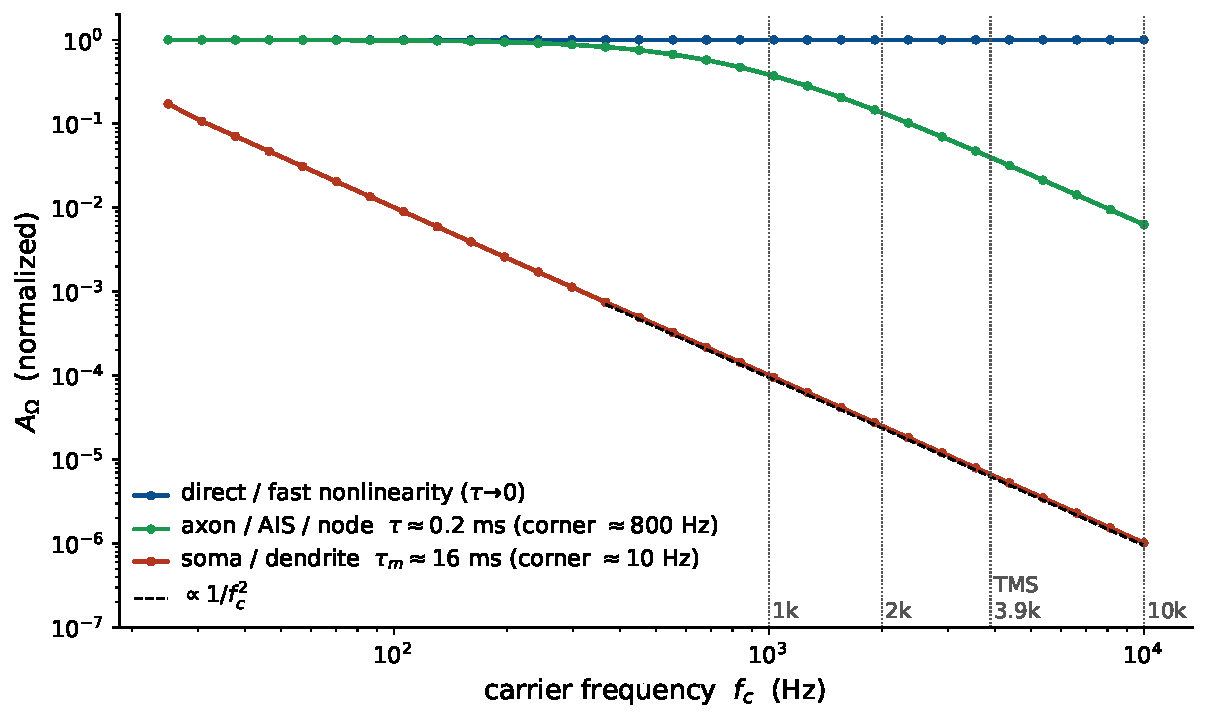
\includegraphics[width=0.74\textwidth]{fig_khz.pdf}
\caption{\textbf{Somatic demodulation dies at kHz, but a fast element survives (Jansen--Rit, open-loop detector).} Open-loop
demodulated response (normalized to the $\tau\!\to\!0$ value) vs.\ carrier
frequency up to $10$~kHz. With direct coupling ($\tau\!\to\!0$) the response is
flat---carrier-independent. A slow somatic membrane ($\tau_m\!\approx\!16$~ms)
rolls off as $1/f_c^2$ (dashed guide), killing kHz demodulation; a fast element
(axon/AIS/node, $\tau\!\approx\!0.2$~ms) retains an appreciable response into the
kHz band ($\sim$0.14 at 2~kHz, $\sim$0.04 at the TMS peak $3.9$~kHz). The same
membrane filter attenuates TMS at the soma, which is why neither TMS nor TI should
be thought of as driving the soma at kHz.}
\label{fig:khz}
\end{figure}
\begin{figure}[t!]
\centering
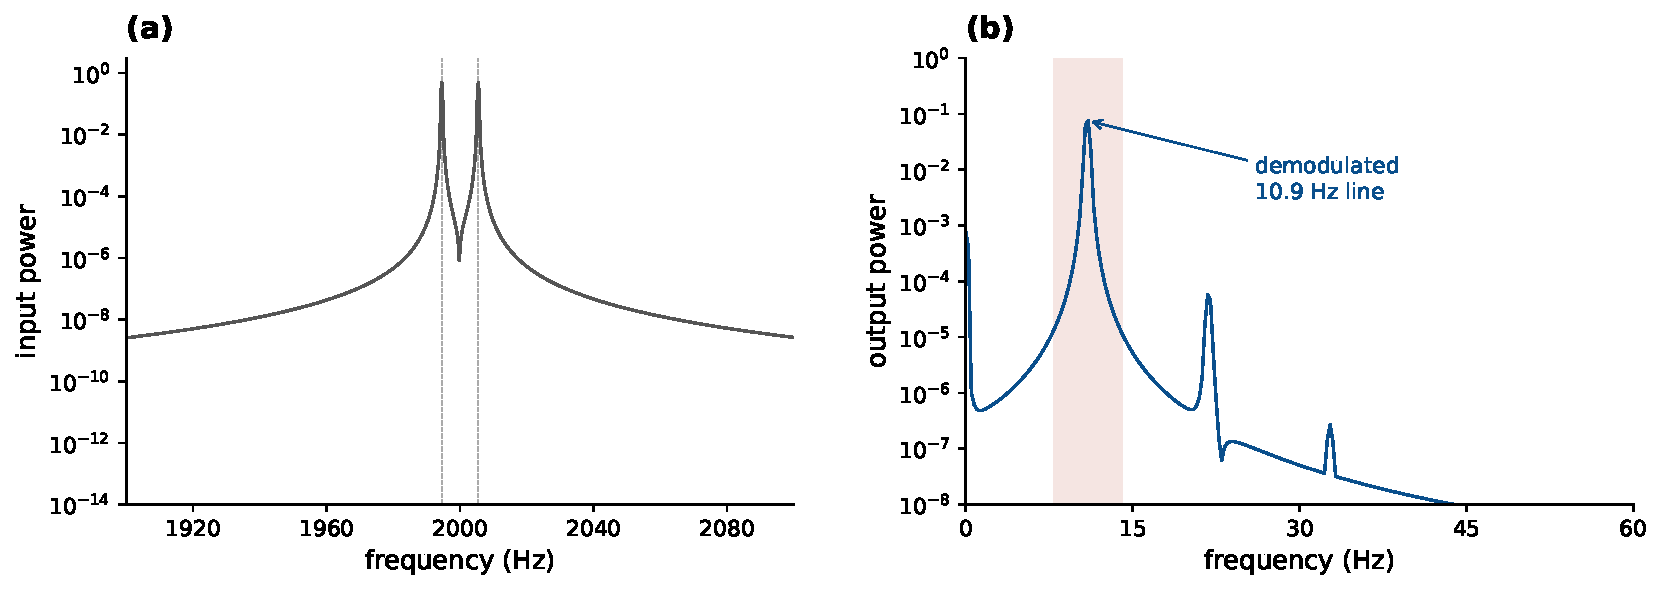
\includegraphics[width=0.95\textwidth]{fig_khz_twotone.pdf}
\caption{\textbf{Genuine two-tone TI at a real kHz carrier (Jansen--Rit, fast-element
route).} Two equal tones at $f_1=1994.5$ and $f_2=2005.5$~Hz, beating at $10.9$~Hz, pass
through the fast-element low-pass ($\tau=0.2$~ms) into the recurrent column.
\emph{(a)} The input spectrum has lines only at $f_1$ and $f_2$; power in the
$8$--$14$~Hz band is $2.2\times10^{-13}$, zero to numerical precision.
\emph{(b)} The output carries a clean demodulated line at $11.0$~Hz. This is the kHz
claim on the physical waveform rather than on the AM surrogate.}
\label{fig:khz_twotone}
\end{figure}
\begin{figure}[t!]
\centering
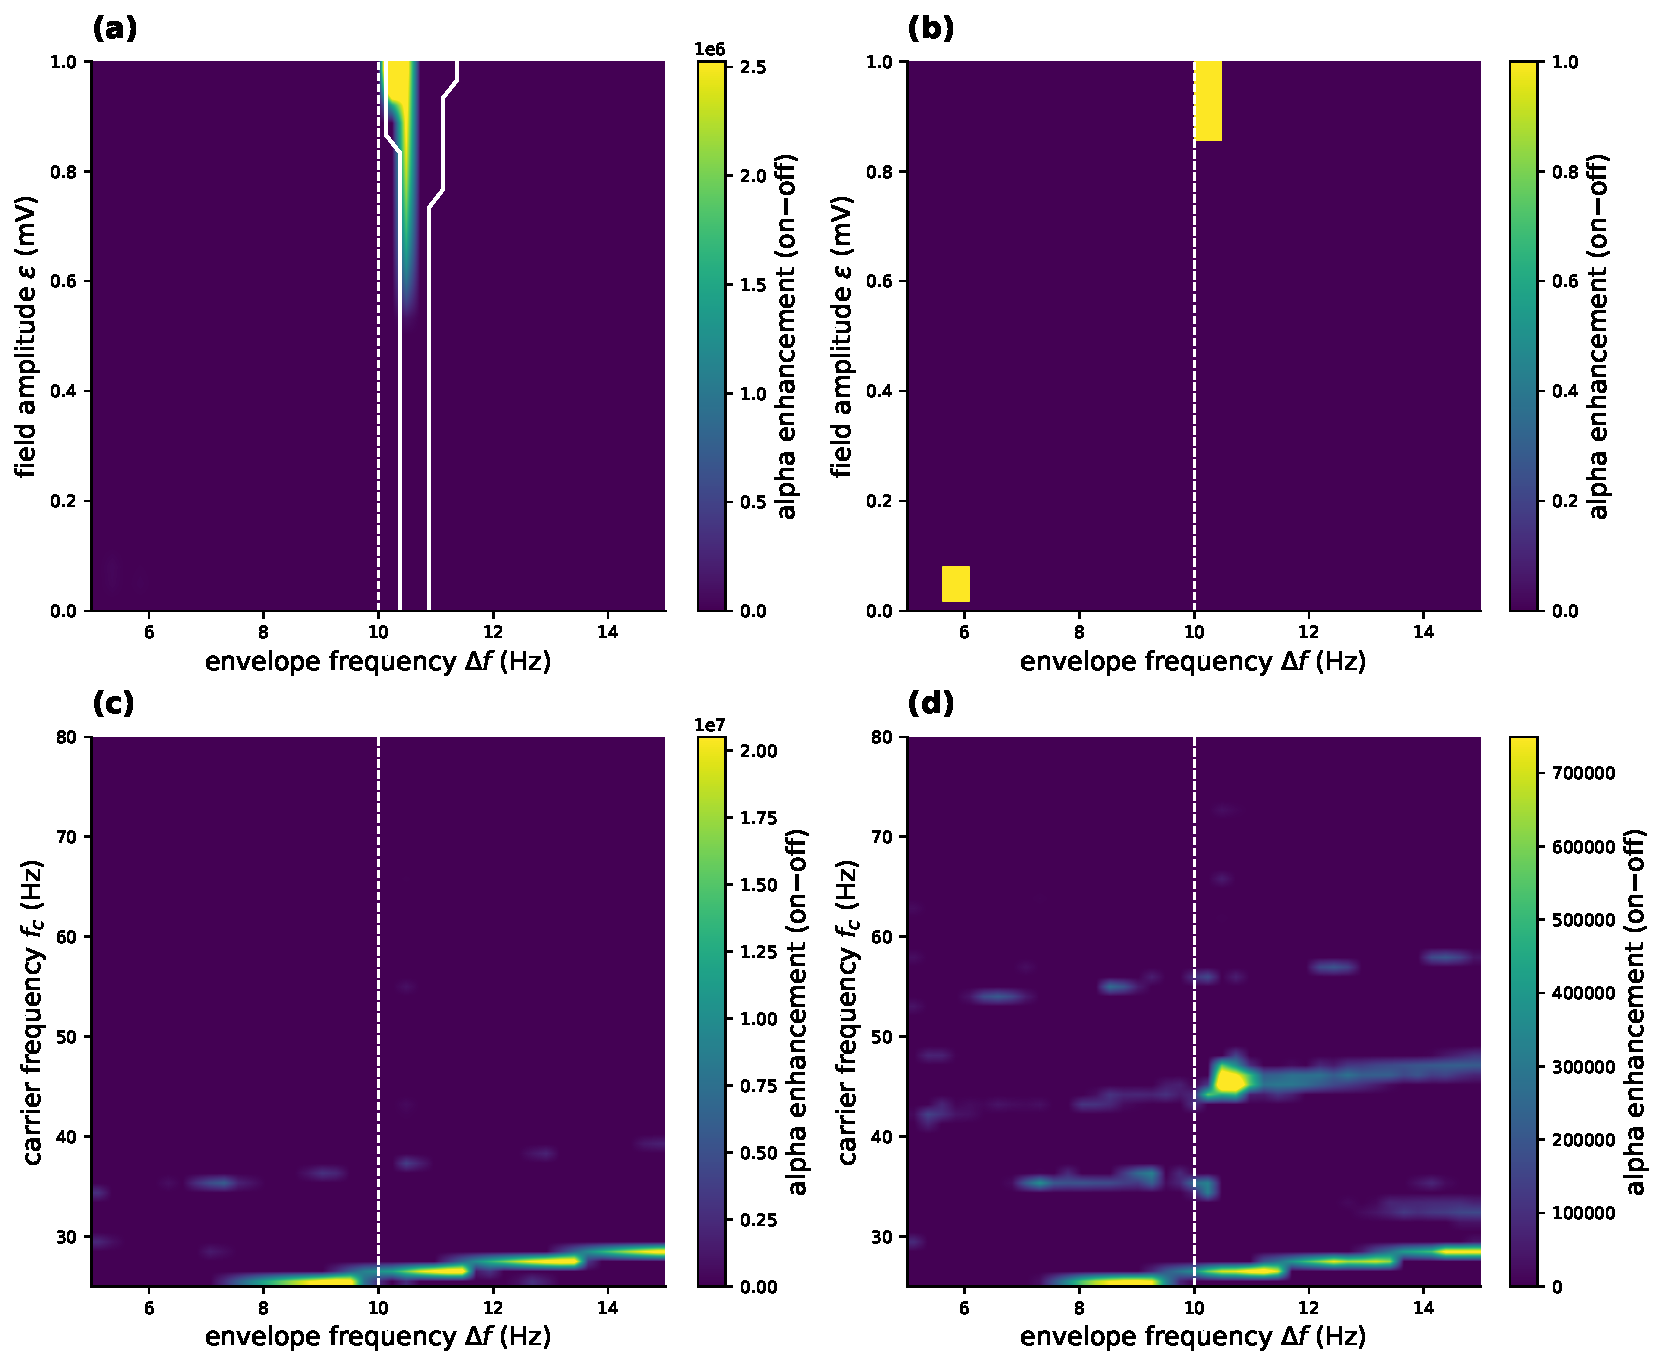
\includegraphics[width=0.86\textwidth]{fig_lanmm_field_p1_twotone.pdf}
\caption{\textbf{LaNMM Arnold tongues: two-tone TI field delivered directly to the deep
$P_1$ (alpha) loop.} As Fig.~\ref{fig:lanmm_p2} but with the field on $P_1$. The deep loop
is captured by a much weaker field than the superficial one, so the amplitude range is
$\varepsilon\le1$~mV here against $3$~mV there; above $\approx$$2$~mV the drive captures
essentially the whole $\Delta f$ sweep and leaves the perturbative regime the theory
describes. Colour: stimulation-induced alpha-band enhancement over the $\varepsilon=0$
baseline. \emph{(a,b)} $P_1$ and $P_2$ enhancement vs.\ $\varepsilon$ and $\Delta f$; the
white contour in \emph{(a)} outlines the $1{:}1$ frequency-captured set,
$|f_{\rm out}-\Delta f|<0.3$~Hz (Appendix~\ref{sec:vocab}), computed from the dominant
output frequency because band power alone cannot separate capture from a forced response.
Its width grows from $0.5$~Hz at $\varepsilon\!\to\!0$ to $1.25$~Hz at $\varepsilon=1$~mV.
\emph{(c,d)} Enhancement vs.\ carrier frequency and $\Delta f$ at $\varepsilon=0.5$~mV.
$P_1$ responds across a \emph{broad} carrier band---a vertical ridge at
$\Delta f\!\approx\!10$~Hz, the direct-coupling limit of Eq.~\eqref{eq:demod}. Read with
the lock-in at $\Delta f$ the response is retained at every carrier from $25$ to $80$~Hz
(median $25\%$ of peak), in contrast to the $\sim$7\% collapse off resonance under
superficial drive.}
\label{fig:lanmm_p1}
\end{figure}
\begin{figure}[t!]
\centering
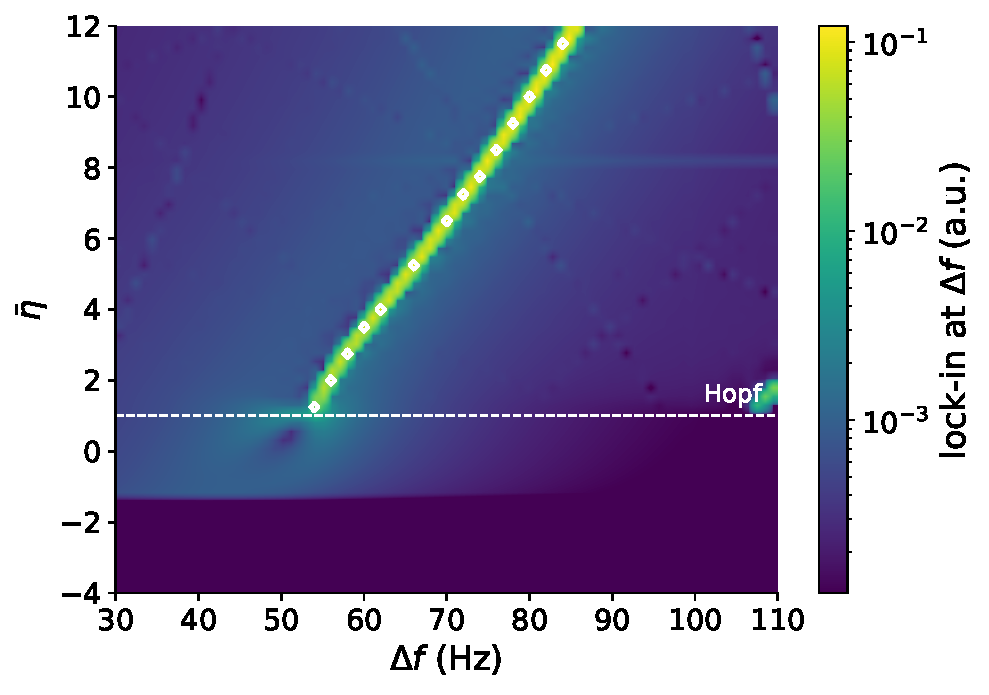
\includegraphics[width=0.72\textwidth]{fig_nmm2_map.pdf}
\caption{\textbf{NMM2 PING resonance map (exact mean field).} Demodulated response over
the ($\Delta f$, background drive $\bar\eta$) plane, log color scale. The ridge follows the
gamma natural frequency, and its diagonal slope---$f_0$ rising with $\bar\eta$---reflects
the state-dependent transfer of NMM2, absent in the static-sigmoid models. White markers
outline the $1{:}1$ captured set (Appendix~\ref{sec:vocab}), drawn only above the Hopf
(dashed line) where there is an autonomous rhythm to capture; below it the same color field
is a forced response. Lock-in amplitude cannot separate the two, since both place power at
$\Delta f$.}
\label{fig:nmm2_map}
\end{figure}


\begin{figure}[t!]
\centering
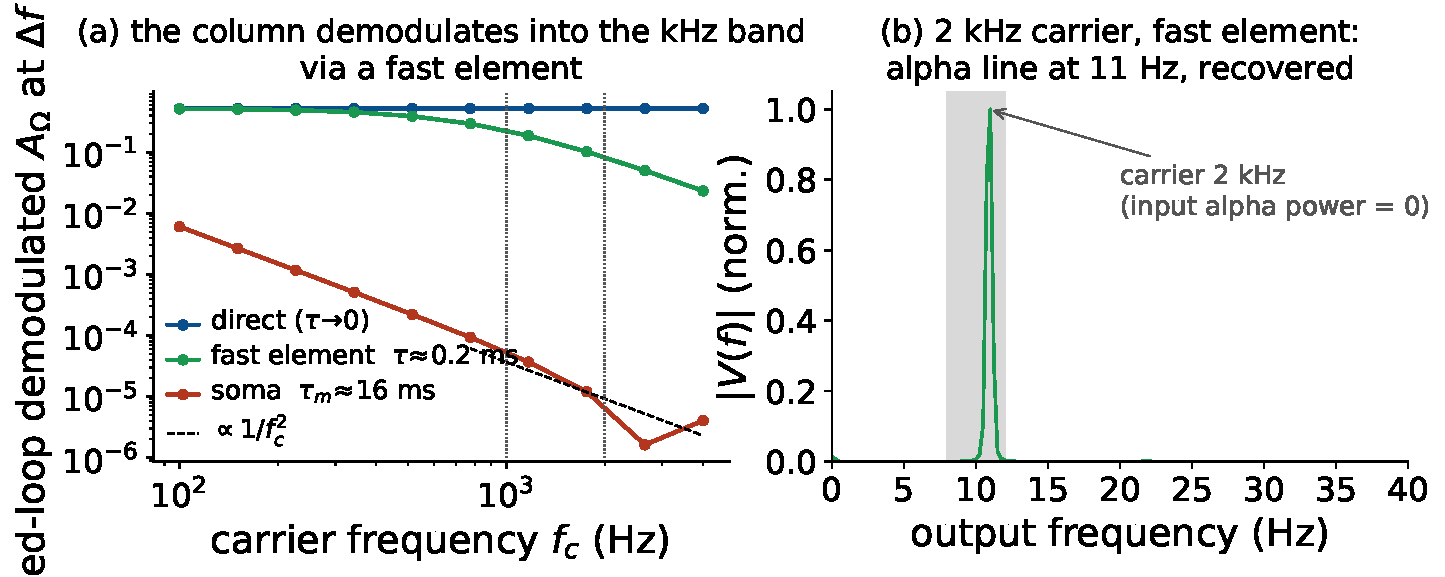
\includegraphics[width=\textwidth]{fig_khz_direct.pdf}
\caption{\textbf{Demodulation at a genuine kHz carrier (Jansen--Rit, closed loop).}
The applied field passes through an explicit membrane filter before the sigmoid.
\emph{(a)} Closed-loop demodulated $A_\Omega$ at $\Delta f=f_0$ vs.\ carrier $f_c$ for
three coupling routes: direct ($\tau\!\to\!0$, carrier-independent), fast element
(axon/AIS/node, $\tau\!\approx\!0.2$~ms; survives into the kHz band), and soma
($\tau_m\!\approx\!16$~ms; collapses as $1/f_c^2$). \emph{(b)} Output spectrum for a
$2$~kHz carrier delivered through the fast element: a clean alpha line at $f_0$,
synthesized by the column although the input carries no alpha power.}
\label{fig:khz_direct}
\end{figure}

\begin{figure}[t!]
\centering
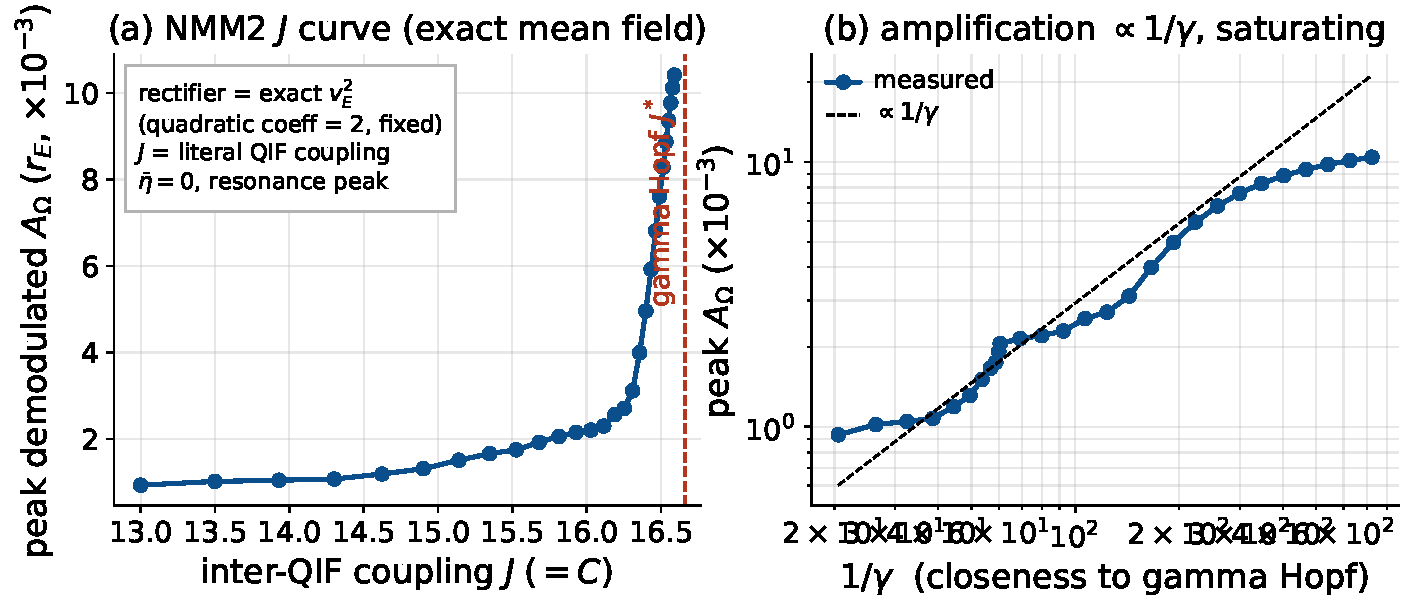
\includegraphics[width=0.92\textwidth]{fig_nmm2_jcurve.pdf}
\caption{\textbf{Coupling controls the amplification in the exact mean field (NMM2
PING, gamma).} $J\,(=C)$ is the literal inter-QIF synaptic weight; the rectifier is the
exact $v_E^2$ (fixed quadratic coefficient), so no operating-point pinning is needed.
\emph{(a)} The peak demodulated response of $r_E$ grows as $J\!\to\!J^*$ (gamma
Hopf, $\bar\eta=0$; stable focus, $\gamma>0$). \emph{(b)} The gain grows as $1/\gamma$ (dashed), saturating near
criticality---the JR law, now with coupling and rectifier both derived.}
\label{fig:nmm2_jcurve}
\end{figure}

\begin{figure}[t!]
\centering
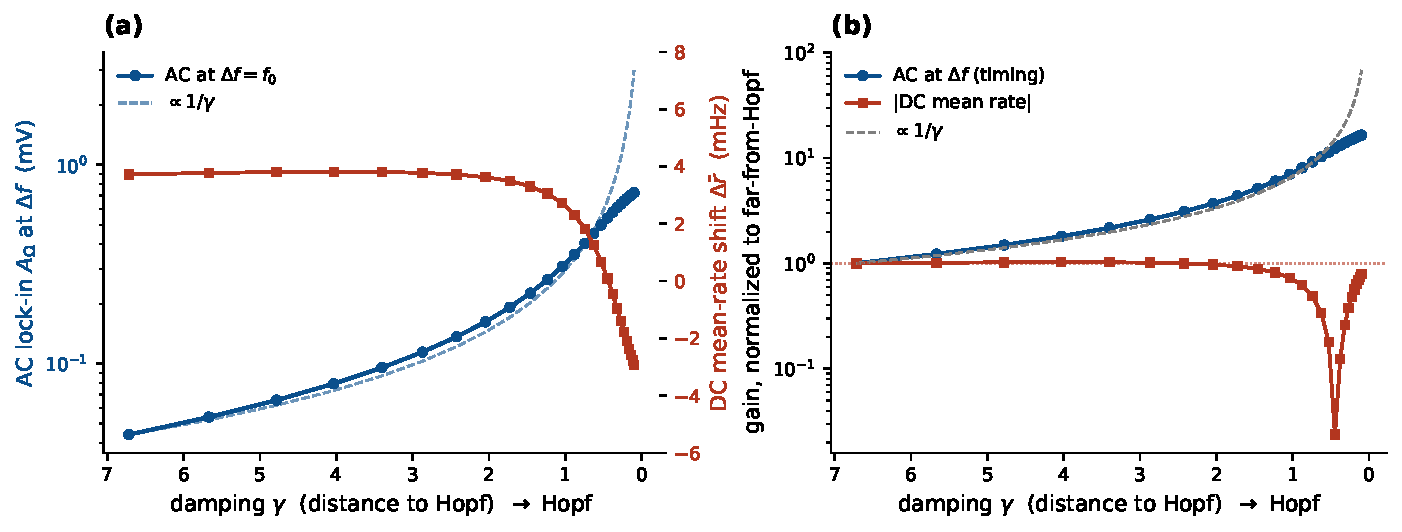
\includegraphics[width=\textwidth]{fig_timing_not_rate.pdf}
\caption{\textbf{Timing, not rate (Jansen--Rit, detection pinned).} As the column is
driven toward the Hopf (from the stable side, $\gamma>0$) through the coupling at fixed $\Sig''(v^*)$, \emph{(a)} the AC
lock-in at the resonant beat $\Delta f=f_0$ (blue) is resonantly amplified and tracks
$1/\gamma$ (dashed), while the DC shift of the mean firing rate (red) stays flat at a
few mHz. \emph{(b)} Normalized to the far-from-Hopf value (log scale): the AC gain
follows $1/\gamma$ and saturates near criticality, whereas the DC gain stays
$\sim$1. The envelope locks timing, not rate---the population analog of the
spike-timing-without-rate finding of \cite{vieira2024}.}
\label{fig:timing}
\end{figure}

\begin{figure}[t!]
\centering
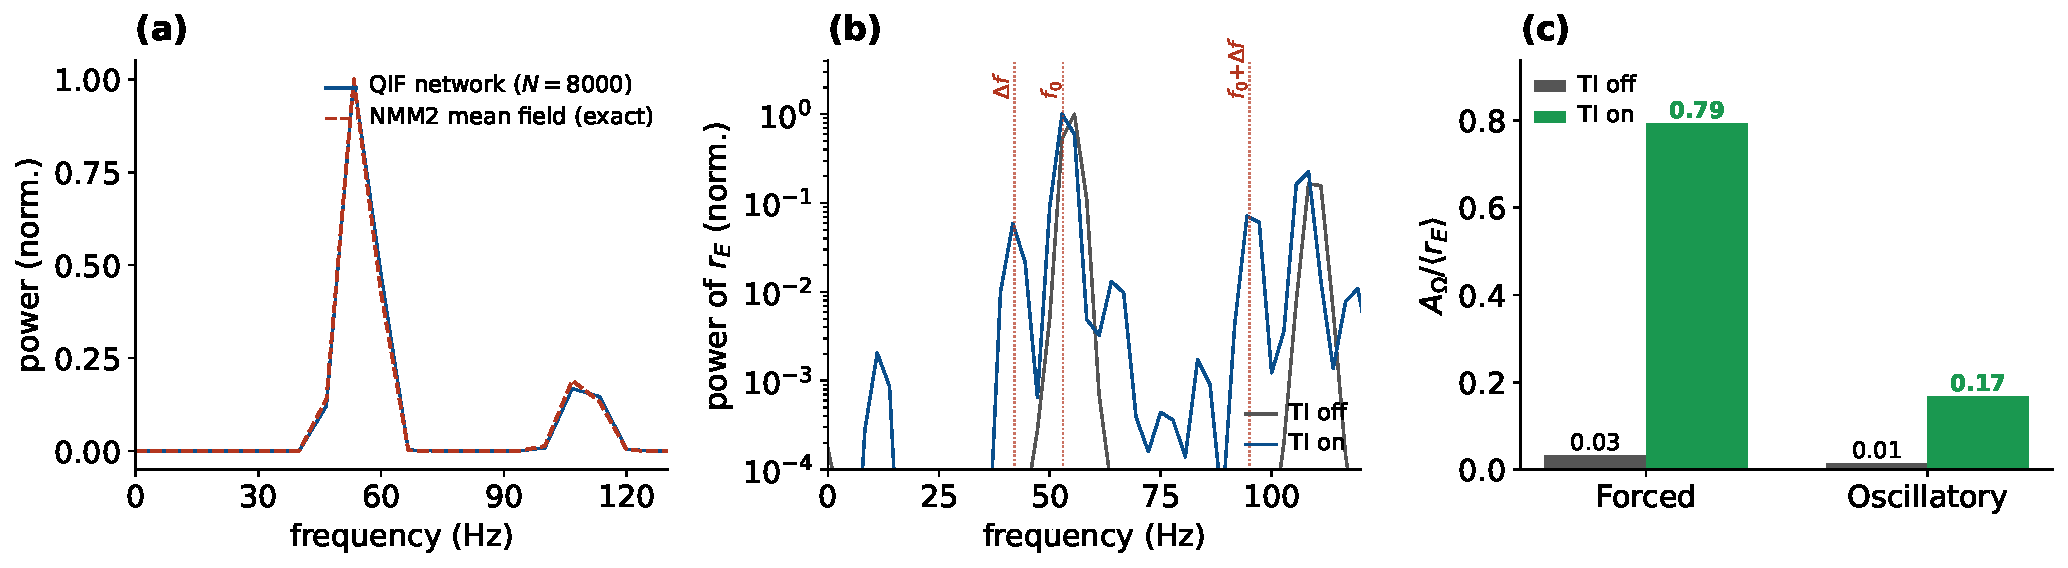
\includegraphics[width=\textwidth]{fig_qif_timing_twotone.pdf}
\caption{\textbf{Timing, not rate, in the QIF network.} \emph{(a)} Field-free power
spectrum of $r_E(t)$: the spiking network ($N=8000$) matches the exact NMM2 mean field in
both gamma frequency ($\sim$53~Hz) and mean rate. \emph{(b)} Intermodulation above the
Hopf (TI off vs.\ on, log power): the nonlinearity mixes the imposed $\Delta f=42$~Hz beat
with the intrinsic $53$~Hz gamma, raising the direct $\Delta f$ line and the sum sideband
near $95$~Hz, both absent with TI off. This is the sideband signature of gating rather
than entrainment. \emph{(c)} The $\Delta f$ modulation depth
$A_\Omega/\langle r_E\rangle$, off vs.\ on: $0.01$--$0.03$ rising to $0.17$--$0.79$, while
the mean rate stays nearly flat ($\times1.07$--$1.11$). Modulation depth is reported
rather than the off$\to$on lock-in ratio, whose denominator sits at the near-zero
field-free floor.}
\label{fig:qif_timing}
\end{figure}


% The supplement cites a handful of works (locking metrics, normal-form theory)
% and is read as a standalone file, so it carries its own reference list.
\ifsupp
\clearpage
\bibliographystyle{unsrt}
\bibliography{references}
\fi
\fi
\end{document}
